\documentclass{article}

% ------------------------ Packages ------------------------
\usepackage{amsmath, amssymb}
\usepackage{tikz}
\usepackage{graphicx}
\usepackage{caption}
\usepackage[margin=1in]{geometry} % 전체 문서: portrait
\usepackage{pdflscape}            % 특정 페이지만 가로(landscape)로
\usetikzlibrary{shapes, arrows, positioning, fit, calc}
\usetikzlibrary{shapes.geometric, arrows.meta, positioning, calc, decorations.pathreplacing}

% Page numbering
\usepackage{fancyhdr}
\pagestyle{fancy}
\fancyhf{}
\fancyfoot[C]{\thepage}
\renewcommand{\headrulewidth}{0pt}

% ------------------------ Document ------------------------
\begin{document}

\title{Transformer Parallelism:\\
       A Visual, Dimension-Oriented Guide}
\author{}
\date{November 4, 2025}
\maketitle

\tableofcontents
\clearpage

% ==========================================================
% 1. Neural Network Basics
% ==========================================================
\section{Neural Network Basics}

In this section, we briefly introduce the core ideas of neural networks
for readers with no prior background. We cover the notion of tensors,
linear layers, activation functions, and the backpropagation algorithm
at a high level.

\subsection{What is a Neural Network?}
Here we describe the basic idea of a neural network as a composition of
linear transformations and non-linear activation functions, operating
on vector or matrix inputs.

\subsection{Fully-Connected Layers and MLPs}
We introduce the multi-layer perceptron (MLP):
\begin{itemize}
  \item Input/output shapes $[B, D]$.
  \item Linear layer $W \in \mathbb{R}^{D_{\text{in}} \times D_{\text{out}}}$,
        bias $b \in \mathbb{R}^{D_{\text{out}}}$.
  \item Activation functions such as ReLU or GELU.
\end{itemize}
This provides the foundation for understanding the Transformer MLP block.

\subsection{Backpropagation at a Glance}
We explain the key idea of backpropagation:
\begin{itemize}
  \item Gradients flowing from the loss to earlier layers.
  \item Parameter updates using optimizers such as SGD or Adam.
\end{itemize}
The detailed backward diagrams in later sections are concrete instances
of this general principle.

\clearpage

% ==========================================================
% 2. From Neural Networks to Transformers
% ==========================================================
\section{From Neural Networks to Transformers}

\subsection{Sequence Modeling Motivation}
We consider sequence modeling tasks such as natural language processing,
time series forecasting, and speech processing. In these settings the
input is not a single vector but a \emph{sequence} of tokens, each of
which is mapped to an embedding. The model must capture dependencies
both between nearby tokens and between tokens that are far apart in
the sequence.

\subsection{The Self-Attention Idea}
Transformers address sequence modeling by using self-attention instead
of explicit recurrence. At a high level:
\begin{itemize}
  \item Each token is mapped to an input embedding.
  \item Self-attention allows every position to attend to every other
        position in the same sequence.
  \item Multi-head attention (MHA) uses several attention ``heads'' in
        parallel to capture different types of relationships.
  \item A position-wise feed-forward network (MLP block) processes each
        token independently after attention.
  \item Layer normalization, residual connections, and an output
        projection tie the blocks together and produce final logits or
        predictions.
\end{itemize}

In the following sections we make these ideas concrete using
dimension-annotated diagrams of a Transformer layer and its parallel
variants.

\clearpage

% ==========================================================
% 3. Notation and Diagram Conventions
% ==========================================================
\section{Notation and Diagram Conventions}

Before diving into layer-wise forward and backward diagrams, we summarize
the notational conventions and visual elements used throughout the paper.
All later figures (single-node, TP, DP, and DP+TP overall flow) follow
these conventions.

\subsection{Tensor Shapes, Indices, and Local Views}

We use the following global symbols and dimensions:
\begin{itemize}
  \item $B$: global batch size.
  \item $S$: sequence length (number of tokens).
  \item $D$: model (hidden) dimension.
  \item $D_{ff}$: intermediate MLP dimension.
  \item $N_H$: number of attention heads.
  \item $D_h$: per-head dimension, typically $D_h = D / N_H$.
  \item $N_T$: tensor-parallel degree (number of TP shards).
  \item $N_D$: data-parallel degree (number of DP replicas).
\end{itemize}

In formulas we write, for example,
\(\mathbf{X} \in \mathbb{R}^{B \times S \times D}\), while in the diagrams
we annotate edges with a compact bracket notation such as \([B,S,D]\).
Throughout the figures we use:
\begin{itemize}
  \item \([B,S,D]\) \(\;\leftrightarrow\;\)
        \(\mathbb{R}^{B \times S \times D}\)
  \item \([B,N_H,S,D_h]\) \(\;\leftrightarrow\;\)
        \(\mathbb{R}^{B \times N_H \times S \times D_h}\)
  \item \([B,N_H,S,S]\) \(\;\leftrightarrow\;\)
        \(\mathbb{R}^{B \times N_H \times S \times S}\)
\end{itemize}

In parallel settings we also show \emph{local} shapes from the point of
view of a single node or shard:
\begin{itemize}
  \item Data parallel (DP): each replica processes a fraction of the batch,
        with local tensors of shape approximately \([B/N_D,S,D]\).
  \item Tensor parallel (TP): hidden or head dimensions are partitioned
        across shards, leading to shapes such as
        \([B,S,D/N_T]\) or \([B,N_H,S,D_h/N_T]\).
\end{itemize}

Thus edge labels such as \([B/N_D,S,D/N_T]\) should be read as
“the tensor shape seen by a single node or shard”.

Typical tensor shapes used in the figures:
\begin{itemize}
  \item $\mathbf{X} \in \mathbb{R}^{B \times S \times D}$:
        input or hidden states (annotated as \([B,S,D]\) on edges).
  \item $\mathbf{H} \in \mathbb{R}^{B \times S \times D}$:
        normalized or intermediate hidden states.
  \item $\mathbf{Q}, \mathbf{K}, \mathbf{V} \in \mathbb{R}^{B \times N_H \times S \times D_h}$:
        query, key, value tensors after projection
        (annotated as \([B,N_H,S,D_h]\)).
  \item $\mathbf{AS} \in \mathbb{R}^{B \times N_H \times S \times S}$:
        attention scores after scaling and softmax
        (annotated as \([B,N_H,S,S]\)).
  \item $\mathbf{Y} \in \mathbb{R}^{B \times S \times D}$:
        output of a Transformer block or layer.
\end{itemize}

Gradients are denoted by a leading \(\mathrm{d}\), e.g.\
\(\mathrm{d}\mathbf{X}\), \(\mathrm{d}\mathbf{W}\),
or \(\mathbf{dA}_{\text{out}}\). In the diagrams we use the same symbols
but typically omit the explicit set notation.

\subsection{Computation Nodes and Local Operations}

All single-node, TP, DP, and DP+TP figures share the same visual
vocabulary for computation nodes.

\paragraph{Matrix multiplication (matmul)}
\begin{itemize}
  \item Symbol: \textbf{circle containing ``\(\bullet\)''} (denoted
        \verb|mulnode| in TikZ).
  \item Meaning: linear operations of the form
        \(\mathbf{A}\mathbf{W}\) or \(\mathbf{W}^{T}\mathbf{A}\).
  \item Examples:
        \begin{itemize}
          \item MHA Q/K/V projections:
                \(\mathbf{Q} = \mathbf{X}_{\text{norm}}\widetilde{\mathbf{W}}_{Q}\),
                \(\mathbf{K} = \mathbf{X}_{\text{norm}}\widetilde{\mathbf{W}}_{K}\),
                \(\mathbf{V} = \mathbf{X}_{\text{norm}}\widetilde{\mathbf{W}}_{V}\).
          \item MLP up/down projections:
                \(\mathbf{H}_{\text{inter}} = \mathbf{H}\widetilde{\mathbf{W}}_{up}\),
                \(\mathbf{Y} = \mathbf{H}_{\text{inter}}\widetilde{\mathbf{W}}_{down}\).
        \end{itemize}
\end{itemize}

\paragraph{Elementwise (bitwise) addition}
\begin{itemize}
  \item Symbol: \textbf{circle containing ``$+$''} (denoted
        \verb|addnode|).
  item Meaning: elementwise addition of tensors with the same shape.
  \item Typical usage:
        \begin{itemize}
          \item bias addition: \(\mathbf{Z} + \mathbf{b}\),
          \item residual connections:
                \(\mathbf{X} + \mathrm{Block}(\mathbf{X})\),
          \item summing multiple gradient contributions:
                \(\mathbf{dX} = \mathbf{dX}_1 + \mathbf{dX}_2 + \dots\).
        \end{itemize}
\end{itemize}

\paragraph{Nonlinear and pointwise operations}
\begin{itemize}
  \item Symbol: \textbf{rectangular node} (often \verb|auxnode|).
  \item Representative labels:
        \begin{itemize}
          \item \texttt{Softmax}, \texttt{dSM}, \texttt{dS}:
                softmax on attention scores and its backward pass.
          \item \texttt{GLU}, \texttt{GELU}, \texttt{ReLU},
                \texttt{dGL}: MLP nonlinearities and their backward passes.
          \item \texttt{LN}, \texttt{dLN}: layer normalization forward / backward.
          \item \texttt{DO}: dropout forward / backward.
        \end{itemize}
  \item These operators act pointwise (or per feature) and typically
        preserve the overall tensor shape.
\end{itemize}

\paragraph{Broadcast (BC)}
\begin{itemize}
  \item Symbol: rectangular node labeled \texttt{BC}.
  \item Meaning: broadcasting a lower-rank tensor along one or more
        dimensions so that it can be added elementwise to a higher-rank
        tensor. A common example is broadcasting a bias
        \(\mathbf{b} \in \mathbb{R}^{D}\) to match a tensor of shape
        \([B,S,D]\).
\end{itemize}

\paragraph{Summation over batch/sequence}
\begin{itemize}
  \item Symbol: \textbf{small circle containing ``\(\sum\)''}
        (denoted \verb|sumnode|).
  \item Meaning: explicit summation over specified axes, typically
        batch and sequence.
  \item Typical use: computing bias gradients such as
        \(\mathrm{d}\tilde{\mathbf{b}} = \sum_{B,S} \mathrm{d}\mathbf{Z}\).
\end{itemize}

\paragraph{Reshape and transpose}
\begin{itemize}
  \item \textbf{R}:
        reshape or dimension reordering operator.
        For example, switching between
        \([B,S,N_H,D_h]\) and \([B,N_H,S,D_h]\).
  \item \textbf{T}:
        transpose operator, often exchanging the last two dimensions,
        e.g.\ \([B,N_H,S,D_h] \rightarrow [B,N_H,D_h,S]\).
\end{itemize}

\subsection{Parallel Groups and Node-Level View}

The DP, TP, and DP+TP overall flow figures show not only layer-internal
operations but also the structure across nodes and shards.

\begin{itemize}
  \item \textbf{Data-parallel replicas}:
        nodes labeled ``Node 0'', ``Node 1'', \dots, ``Node $N_D-1$''
        form a DP group. Each replica holds a full copy of the model
        parameters but processes a different slice of the batch.
        Local tensors are typically annotated as \([B/N_D,S,D]\).
  \item \textbf{Tensor-parallel shards}:
        within a node (or within a TP group) weight matrices or hidden
        dimensions are split across \(N_T\) shards.
        Local hidden states may be annotated as \([B,S,D/N_T]\) or
        \([B,N_H,S,D_h/N_T]\).
  \item \textbf{Hybrid DP+TP}:
        in the DP+TP overall flow, each data-parallel replica contains
        a tensor-parallel group. TP communication happens inside each
        replica, while DP communication happens across replicas.
\end{itemize}

\subsection{Arrow Styles, Communication, and Cost Annotations}

\paragraph{Activation and gradient flow}
\begin{itemize}
  \item \textbf{Solid arrows}:
        forward activations (e.g.\ \(\mathbf{X} \rightarrow \mathbf{H}\)).
  \item \textbf{Dashed arrows}:
        backward gradients (e.g.\ \(\mathrm{d}\mathbf{Y} \rightarrow \mathrm{d}\mathbf{X}\)).
  \item \textbf{Double arrows}:
        reuse of cached tensors from the forward pass, such as weights
        or attention scores read again during the backward pass.
\end{itemize}

\paragraph{Collective communication (AR / AG)}

Tensor-parallel (e.g.\ MHA backward under TP) and data-parallel
(e.g.\ DP and DP+TP overall flow) figures contain explicit collective
communication nodes:

\begin{itemize}
  \item \textbf{AR} (All-Reduce): rectangular node labeled \texttt{AR}.
        All nodes in a group exchange local tensors, compute a global
        reduction (typically sum or mean), and receive the reduced
        result. For example, shard-wise weight gradients
        \(\mathbf{d}\widetilde{\mathbf{W}}_{Q}^{(t)}\) are all-reduced
        to form the global gradient.
  \item \textbf{AG} (All-Gather): rectangular node labeled \texttt{AG}.
        Each shard contributes a slice of a tensor; the full tensor is
        reconstructed by concatenation and made available to all shards.
        A typical example is gathering TP-partitioned hidden states or
        attention outputs.
\end{itemize}

\paragraph{DP vs TP communication in DP+TP overall flow}

In the DP+TP overall flow diagram we distinguish carefully between
data-parallel and tensor-parallel communication:

\begin{itemize}
  \item \textbf{DP communication}:
        All-Reduce across data-parallel replicas, usually for weight
        gradients. Edge annotations may show both the local payload
        shape and an algorithm-dependent cost, e.g.
        \[
          \text{Naive: } 2(N_D - 1) \times [B/N_D,S,D],\quad
          \text{Ring: } 2\frac{N_D - 1}{N_D} \times [B/N_D,S,D].
        \]
  \item \textbf{TP communication}:
        All-Reduce or All-Gather across tensor-parallel shards inside
        a node or TP group, with shapes such as \([B,S,D/N_T]\) or
        \([B,N_H,S,D_h/N_T]\).
\end{itemize}

In all cases, the bracket notation on communication edges (for example
\([B,S,D]\) or \([B/N_D,S,D/N_T]\)) indicates the shape of the tensor
sent or received by a \emph{single} node or shard. This makes it
possible to reason about the communication volume and compare DP, TP,
and DP+TP schemes in a consistent way.

\clearpage

% ==========================================================
% 4. Single-Node Transformer: Forward and Backward
% ==========================================================
\section{Single-Node Transformer: Forward and Backward}

This section presents the full Transformer layer running on a single node
(no parallelism). We emphasize tensor shapes and data flow for both
forward and backward passes.

\subsection{Overall Transformer Layer Flow}
\resizebox{\linewidth}{!}{%
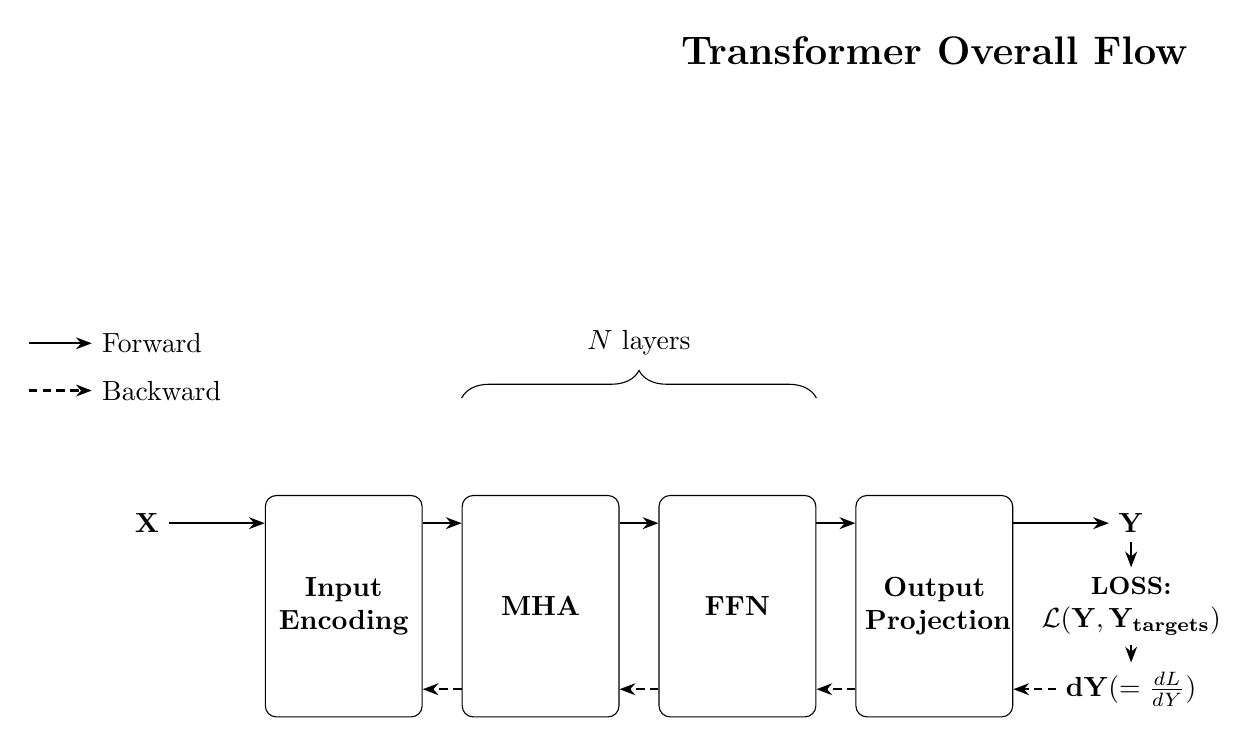
\begin{tikzpicture}[
    node distance=2.5cm,
    >=stealth,
    block/.style={rectangle, draw=black, fill=white, text width=5em, text centered, rounded corners, minimum height=8em, font=\bfseries},
    forward/.style={-{Stealth[length=2mm]}, thick, black},
    backward/.style={-{Stealth[length=2mm]}, thick, black, densely dashed},
    io/.style={text centered, font=\bfseries}
]
    % Title
    \node[font=\Large\bfseries] at (10, 6) {Transformer Overall Flow};

    % Forward path nodes (horizontal)
    \node (input) [io] {$\mathbf{X}$};
    \node (encoding) [block, right of=input, yshift=-3em] {Input\\Encoding};
    \node (mha) [block, right of=encoding] {MHA};
    \node (mlp) [block, right of=mha] {FFN};
    \node (output) [block, right of=mlp] {Output\\Projection};
    \node (pred) [io, right of=output, yshift=3em] {$\mathbf{Y}$};
    \node (loss) [align=center, io, right of=output] {\small LOSS:\\$\mathcal{L}(\mathbf{Y,Y_\text{targets}})$};
    \node (gradient) [io, right of=output, yshift=-3em] {$\mathbf{dY}(=\frac{dL}{dY})$};

    % Forward arrows (upper part of blocks)
    \draw [forward] (input) -- ([yshift=3em]encoding.west);
    \draw [forward] ([yshift=3em]encoding.east) -- ([yshift=3em]mha.west);
    \draw [forward] ([yshift=3em]mha.east) -- ([yshift=3em]mlp.west);
    \draw [forward] ([yshift=3em]mlp.east) -- ([yshift=3em]output.west);
    \draw [forward] ([yshift=3em]output.east) -- (pred);
    \draw [forward] (pred) -- (loss);
    \draw [backward] (loss) -- (gradient);

    % Backward arrows (lower part of blocks)
    \draw [backward] (gradient) -- ([yshift=-3em]output.east);
    \draw [backward] ([yshift=-3em]output.west) -- ([yshift=-3em]mlp.east);
    \draw [backward] ([yshift=-3em]mlp.west) -- ([yshift=-3em]mha.east);
    \draw [backward] ([yshift=-3em]mha.west) -- ([yshift=-3em]encoding.east);

    % Brace for layer repetition
    \draw[decorate, decoration={brace, amplitude=10pt}]
        ([yshift=3.5em]mha.north west) -- ([yshift=3.5em]mlp.north east)
        node[midway, above=12pt, font=\normalsize] {$N$ layers};

    % Labels (Legend)
    \coordinate (legend) at ([xshift=-1.5cm, yshift=6.5em]input);
    \draw[forward] (legend) -- ++(0.8,0) node[right, font=\normalsize] {Forward};
    \draw[backward] ([yshift=-0.6cm]legend) -- ++(0.8,0) node[right, font=\normalsize] {Backward};

\end{tikzpicture}%
}

\clearpage

% ------------------------ 4.1 Input Embedding ------------------------
\subsection{Input Embedding Layer}

\subsubsection{Forward Pass}
\documentclass{article}

\usepackage{amsmath, amssymb}
\usepackage{tikz}
\usepackage{graphicx}
\usepackage{caption}
\usepackage[margin=1in, landscape]{geometry}
\usetikzlibrary{shapes, arrows, positioning, fit, calc}

\begin{document}

% ---------- Input Embedding -> (to MHA) ----------
\noindent
\resizebox{\linewidth}{!}{%
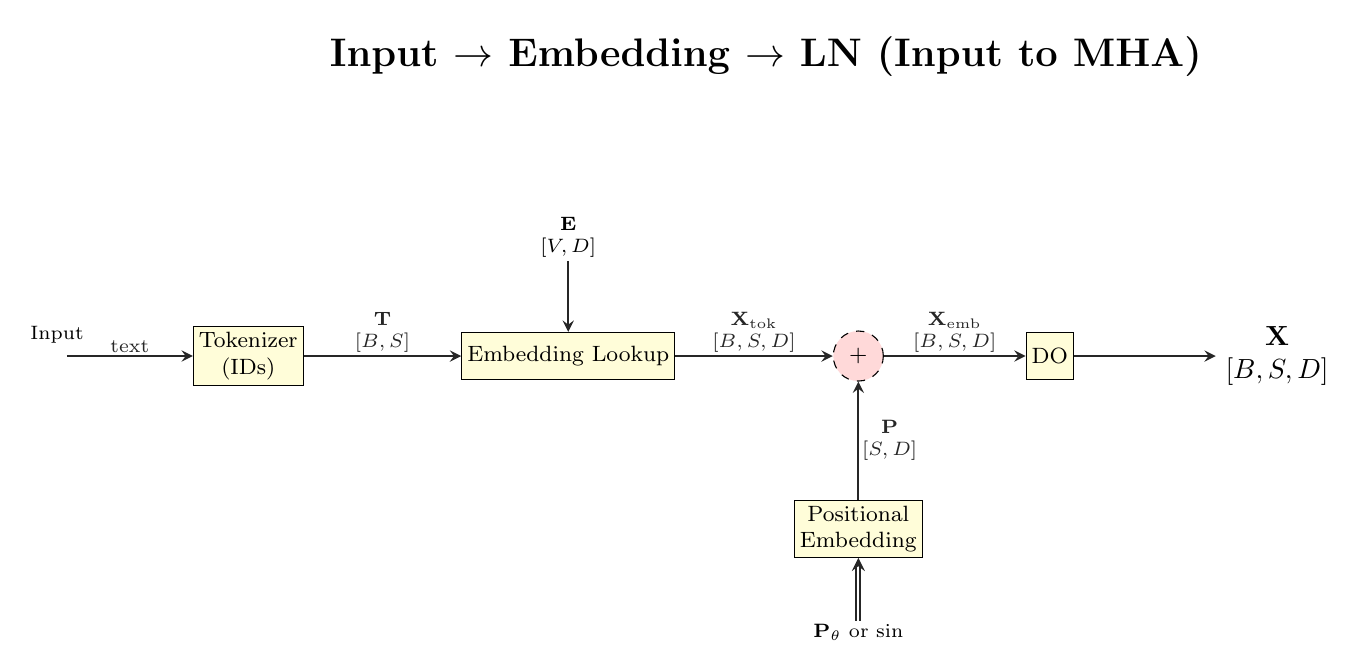
\begin{tikzpicture}[
  >=stealth,
  auxnode/.style={draw, rectangle, fill=yellow!15, minimum height=6mm, inner sep=2pt, font=\footnotesize, align=center},
  mulnode/.style={draw, circle, fill=green!15, minimum size=6mm, font=\footnotesize, align=center},
  addnode/.style={draw, circle, dashed, fill=red!15, minimum size=6mm, font=\footnotesize, align=center},
  flow/.style={->, thick, black!85},
  flow2/.style={->, double, thick, black!85},
  dimlabel/.style={font=\scriptsize, inner sep=1pt, align=center}
]

\node[font=\Large\bfseries] at (9, 3.8) {Input $\rightarrow$ Embedding $\rightarrow$ LN (Input to MHA)};

% nodes
\node (RawText) at (0,0) {};
\node[auxnode, align=center] (Tok)   [right=1.6cm of RawText] {Tokenizer\\(IDs)};
\node[auxnode, align=center] (Lookup)[right=2.0cm of Tok]     {Embedding Lookup};
\node[addnode, minimum size=6mm] (Sum) [right=2.0cm of Lookup] {+};
\node[auxnode, align=center] (PosE)  [below=1.5cm of Sum]  {Positional\\Embedding};
\node[auxnode] (Drop) [right=1.8cm of Sum] {DO};
\node (OUTPUT)   [align=center, right=1.8cm of Drop]   {$\mathbf{X}$\\$[B,S,D]$};

% parameter/const “double” edges
\node[dimlabel] (Eparam) [align=center, above=0.9cm of Lookup] {$\mathbf{E}$\\$[V,D]$};
\node[dimlabel] (Pparam) [align=center, below=0.8cm of PosE]   {$\mathbf{P}_{\theta}$ or sin};

% flows
\draw[flow] (RawText) -- (Tok) node[dimlabel, midway, above]
  {$\text{text}$};
\draw[flow] (Tok) -- (Lookup) node[dimlabel, midway, above]
  {$\mathbf{T}$\\$[B,S]$};

% Embedding matrix E
\draw[flow] (Eparam) -- (Lookup);

% Lookup -> Sum (token embeddings)
\draw[flow] (Lookup) -- (Sum) node[dimlabel, midway, above]
  {$\mathbf{X}_{\text{tok}}$\\$[B,S,D]$};

% Positional embedding path
\draw[flow] (PosE) -- (Sum) node[dimlabel, midway, right]
  {$\mathbf{P}$\\$[S,D]$};

% Optional: show P as parameter (sinusoidal/learned)
\draw[flow2] (Pparam) -- (PosE) ;

\draw[flow] (Sum) -- (Drop) node[dimlabel, midway, above]
  {$\mathbf{X}_{\text{emb}}$\\$[B,S,D]$};
\draw[flow] (Drop) -- (OUTPUT);

% labels for start and destination
\node[dimlabel, above=0.0cm of RawText] {Input};

\end{tikzpicture}%
}

\newpage
\renewcommand{\arraystretch}{1.2}
\small

% -------- Operations (Ops) --------
\begin{center}
\textbf{Operations (Ops)}
\begin{tabular}{llll}
\hline
\textbf{Abbrev} & \textbf{Name} & \textbf{Type / Shape} & \textbf{Notes} \\
\hline
Tokenizer & Tokenizer (IDs) & op & Maps raw text $\to$ integer ids $\mathbf{T}\in\mathbb{Z}^{[B,S]}$. \\
Embedding Lookup & Embedding Lookup & op & Gathers rows from $\mathbf{E}\in\mathbb{R}^{V\times D}$ using ids $\mathbf{T}$. \\
$+$ & Element-wise Add (dashed circle) & op & Adds token and positional embeddings; broadcasting over $B,S$ if needed. \\
DO & Dropout & op & Training-time stochastic dropout on $\mathbf{X}_{\text{emb}}$; identity at inference. \\
\textit{(none)} & Broadcast $\mathrm{BC}_{B,S}(\cdot)$ & op & Expands $[S,D]$ (or $[D]$) to $[B,S,D]$ across batch/sequence. \\
\hline
\end{tabular}
\end{center}

\vspace{0.8em}

% -------- Data Tensors (Values) --------
\begin{center}
\textbf{Data Tensors (Values)}
\begin{tabular}{llll}
\hline
\textbf{Symbol} & \textbf{Name} & \textbf{Shape} & \textbf{Notes} \\
\hline
text & Raw input text & — & Character/byte stream before tokenization. \\
$\mathbf{T}$ & Token ids & $[B,S]$ & Output of Tokenizer; integers in $\{0,\dots,V{-}1\}$. \\
$\mathbf{E}$ & Embedding matrix (params) & $[V,D]$ & Trainable; each vocab entry has a $D$-dim vector. \\
$\mathbf{X}_{\text{tok}}$ & Token embeddings & $[B,S,D]$ & $\mathrm{lookup}(\mathbf{E}, \mathbf{T})$. \\
$\mathbf{P}$ & Positional embedding & $[S,D]$ (or $[B,S,D]$) & Learned $\mathbf{P}_\theta$ \textbf{or} sinusoidal (fixed); broadcast to $[B,S,D]$. \\
$\mathbf{X}_{\text{emb}}$ & Sum of token+pos & $[B,S,D]$ & $\mathbf{X}_{\text{tok}} + \mathrm{BC}_{B,S}(\mathbf{P})$. \\
$\mathbf{X}$ & Input to MHA & $[B,S,D]$ & After dropout (DO); goes to LN/MHA stack. \\
$\mathbf{P}_\theta$ & Learned pos. params & matches $\mathbf{P}$ & Used when positions are trainable; otherwise “sin” denotes fixed sinusoidal. \\
\hline
\multicolumn{4}{l}{\textbf{Shape symbols:}\; $B$=batch size,\; $S$=sequence length,\; $D$=model dim,\; $V$=vocab size.} \\
\multicolumn{4}{l}{\textbf{Notes:}\; In practice, $\mathbf{P}$ may be pre-broadcast to $[B,S,D]$ or added per-token with implicit broadcasting.} \\
\hline
\end{tabular}
\end{center}

\end{document}


\clearpage

\clearpage

% ------------------------ 4.2 Multi-Head Attention -------------------
\subsection{Multi-Head Attention (MHA)}

Multi-Head Attention enables the model to jointly attend to information
from different representation subspaces.

\subsubsection{Forward Pass}

\begin{landscape}
\thispagestyle{fancy}
\resizebox{\linewidth}{!}{%
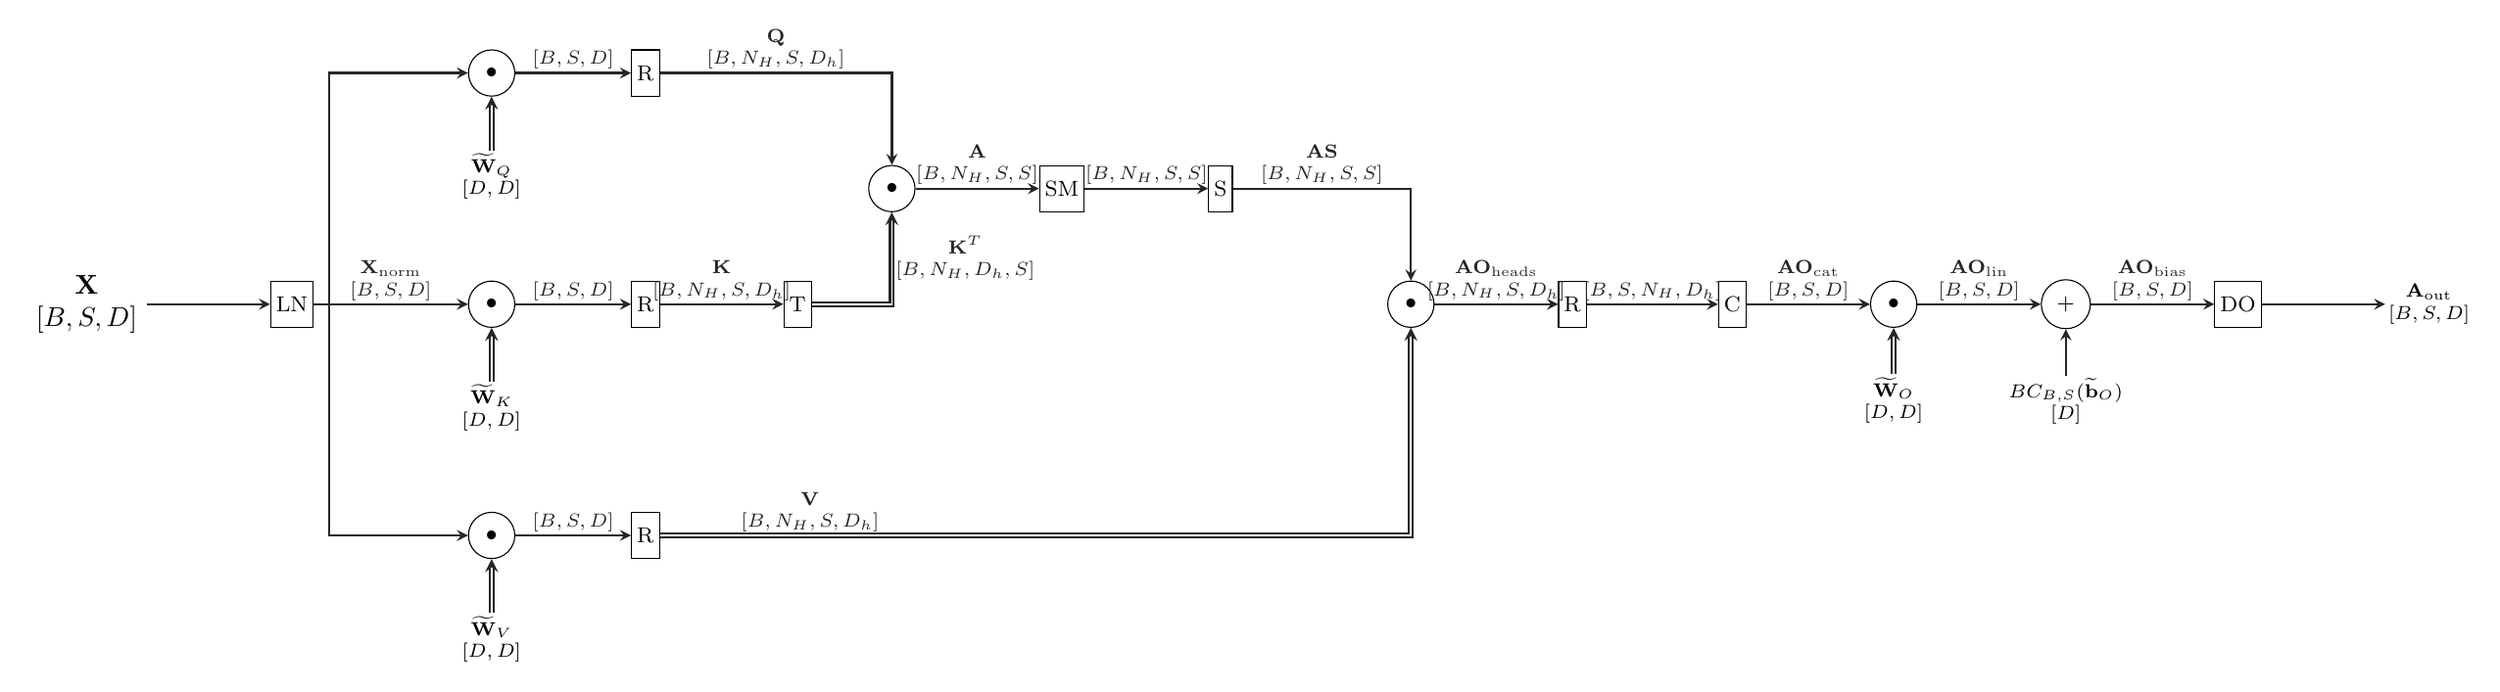
\begin{tikzpicture}[
  every node/.style={transform shape},
  >=stealth,
  auxnode/.style={draw, rectangle, fill=white, minimum height=6mm, inner sep=2pt, font=\footnotesize, align=center},
  mulnode/.style={draw, circle, fill=white, minimum size=6mm, font=\footnotesize, align=center},
  addnode/.style={draw, circle, fill=white, minimum size=6mm, font=\footnotesize, align=center},
  flow/.style={->, thick, black!85},
  flow2/.style={->, double, thick, black!85},
  dimlabel/.style={font=\scriptsize, inner sep=1pt, align=center}
]
% \node[font=\Large\bfseries] at (8, 4.5) {Multi-Head Attention Forward Pass};

\node (Input) at (0.5, 0) [align=center] {$\mathbf{X}$\\$[B,S,D]$};
\node[auxnode] (LN) [right=1.6cm of Input] {LN};

\node[mulnode] (Proj_Q) [right=2.0cm of LN, yshift=3.0cm] {$\bullet$};
\node[auxnode] (R_Q) [right=1.5cm of Proj_Q] {R};

\node[mulnode] (Proj_K) [right=2.0cm of LN, yshift=0cm] {$\bullet$};
\node[auxnode] (R_K) [right=1.5cm of Proj_K] {R};

\node[mulnode] (Proj_V) [right=2.0cm of LN, yshift=-3.0cm] {$\bullet$};
\node[auxnode] (R_V) [right=1.5cm of Proj_V] {R};

\node[dimlabel] (WQ) [align=center, below=0.7cm of Proj_Q] {$\widetilde{\mathbf{W}}_{Q}$\\$[D,D]$};
\node[dimlabel] (WK) [align=center, below=0.7cm of Proj_K] {$\widetilde{\mathbf{W}}_{K}$\\$[D,D]$};
\node[dimlabel] (WV) [align=center, below=0.7cm of Proj_V] {$\widetilde{\mathbf{W}}_{V}$\\$[D,D]$};

\node[auxnode] (T_K) [right=1.6cm of R_K] {T};
\node[mulnode] (QK) [right=2.7cm of R_Q, yshift=-1.5cm] {$\bullet$};
\node[auxnode] (SM) [right=1.6cm of QK] {SM};
\node[auxnode] (Soft) [right=1.6cm of SM] {S};
\node[mulnode] (PV) [right=2.0cm of Soft, yshift=-1.5cm] {$\bullet$};

\node[auxnode] (R_Merge) [right=1.6cm of PV] {R};
\node[auxnode] (Cat) [right=1.7cm of R_Merge] {C};

\node[mulnode] (OProj) [right=1.6cm of Cat] {$\bullet$};
\node[dimlabel] (WO_FWD) [align=center, below=0.6cm of OProj] {$\widetilde{\mathbf{W}}_{O}$\\$[D,D]$};
\node[addnode] (AddB) [right=1.6cm of OProj] {+};
\node[dimlabel] (BO) [align=center, below=0.6cm of AddB] {$BC_{B,S}(\widetilde{\mathbf{b}}_{O})$\\$[D]$};
\node[auxnode] (Drop) [right=1.6cm of AddB] {DO};
\node[dimlabel] (Aout) [align=center, right=1.6cm of Drop] {$\mathbf{A}_{\text{out}}$\\$[B,S,D]$};

\draw[flow] (Input) -- (LN);

\draw[flow] (LN.east) -- ++(0.2,0) |- (Proj_Q.west);
\draw[flow] (LN) -- (Proj_K.west) node[dimlabel, midway, above]{$\mathbf{X}_{\text{norm}}$\\$[B,S,D]$};
\draw[flow] (LN.east) -- ++(0.2,0) |- (Proj_V.west);

\draw[flow2] (WQ) -- (Proj_Q);
\draw[flow2] (WK) -- (Proj_K);
\draw[flow2] (WV) -- (Proj_V);

\draw[flow] (Proj_Q) -- (R_Q) node[dimlabel, midway, above]{$[B,S,D]$};
\draw[flow] (Proj_K) -- (R_K) node[dimlabel, midway, above]{$[B,S,D]$};
\draw[flow] (Proj_V) -- (R_V) node[dimlabel, midway, above]{$[B,S,D]$};

\draw[flow] (R_Q) -| (QK) node[dimlabel, near start, above]{$\mathbf{Q}$\\$[B,N_H,S,D_h]$};
\draw[flow] (R_K) -- (T_K) node[dimlabel, midway, above]{$\mathbf{K}$\\$[B,N_H,S,D_h]$};
\draw[flow2] (T_K) -| (QK) node[dimlabel, near end, right]{$\mathbf{K}^{T}$\\$[B,N_H,D_h,S]$};

\draw[flow] (QK) -- (SM) node[dimlabel, midway, above]{$\mathbf{A}$\\$[B,N_H,S,S]$};
\draw[flow] (SM) -- (Soft) node[dimlabel, midway, above]{$[B,N_H,S,S]$};
\draw[flow] (Soft) -| (PV) node[dimlabel, near start, above]{$\mathbf{AS}$\\$[B,N_H,S,S]$};
\draw[flow2] (R_V) -| (PV) node[dimlabel, pos=0.1, above]{$\mathbf{V}$\\$[B,N_H,S,D_h]$};

\draw[flow] (PV) -- (R_Merge) node[dimlabel, midway, above]{$\mathbf{AO}_{\text{heads}}$\\$[B,N_H,S,D_h]$};
\draw[flow] (R_Merge) -- (Cat) node[dimlabel, midway, above]{$[B,S,N_H,D_h]$};
\draw[flow] (Cat) -- (OProj) node[dimlabel, midway, above]{$\mathbf{AO}_{\text{cat}}$\\$[B,S,D]$};
\draw[flow2] (WO_FWD) -- (OProj);
\draw[flow] (OProj) -- (AddB) node[dimlabel, midway, above]{$\mathbf{AO}_{\text{lin}}$\\$[B,S,D]$};
\draw[flow] (BO) -- (AddB);
\draw[flow] (AddB) -- (Drop) node[dimlabel, midway, above]{$\mathbf{AO}_{\text{bias}}$\\$[B,S,D]$};
\draw[flow] (Drop) -- (Aout);
\end{tikzpicture}%
}

\end{landscape}
\clearpage

\subsubsection{Backward Pass}

\begin{landscape}
\thispagestyle{fancy}
\resizebox{\linewidth}{!}{%
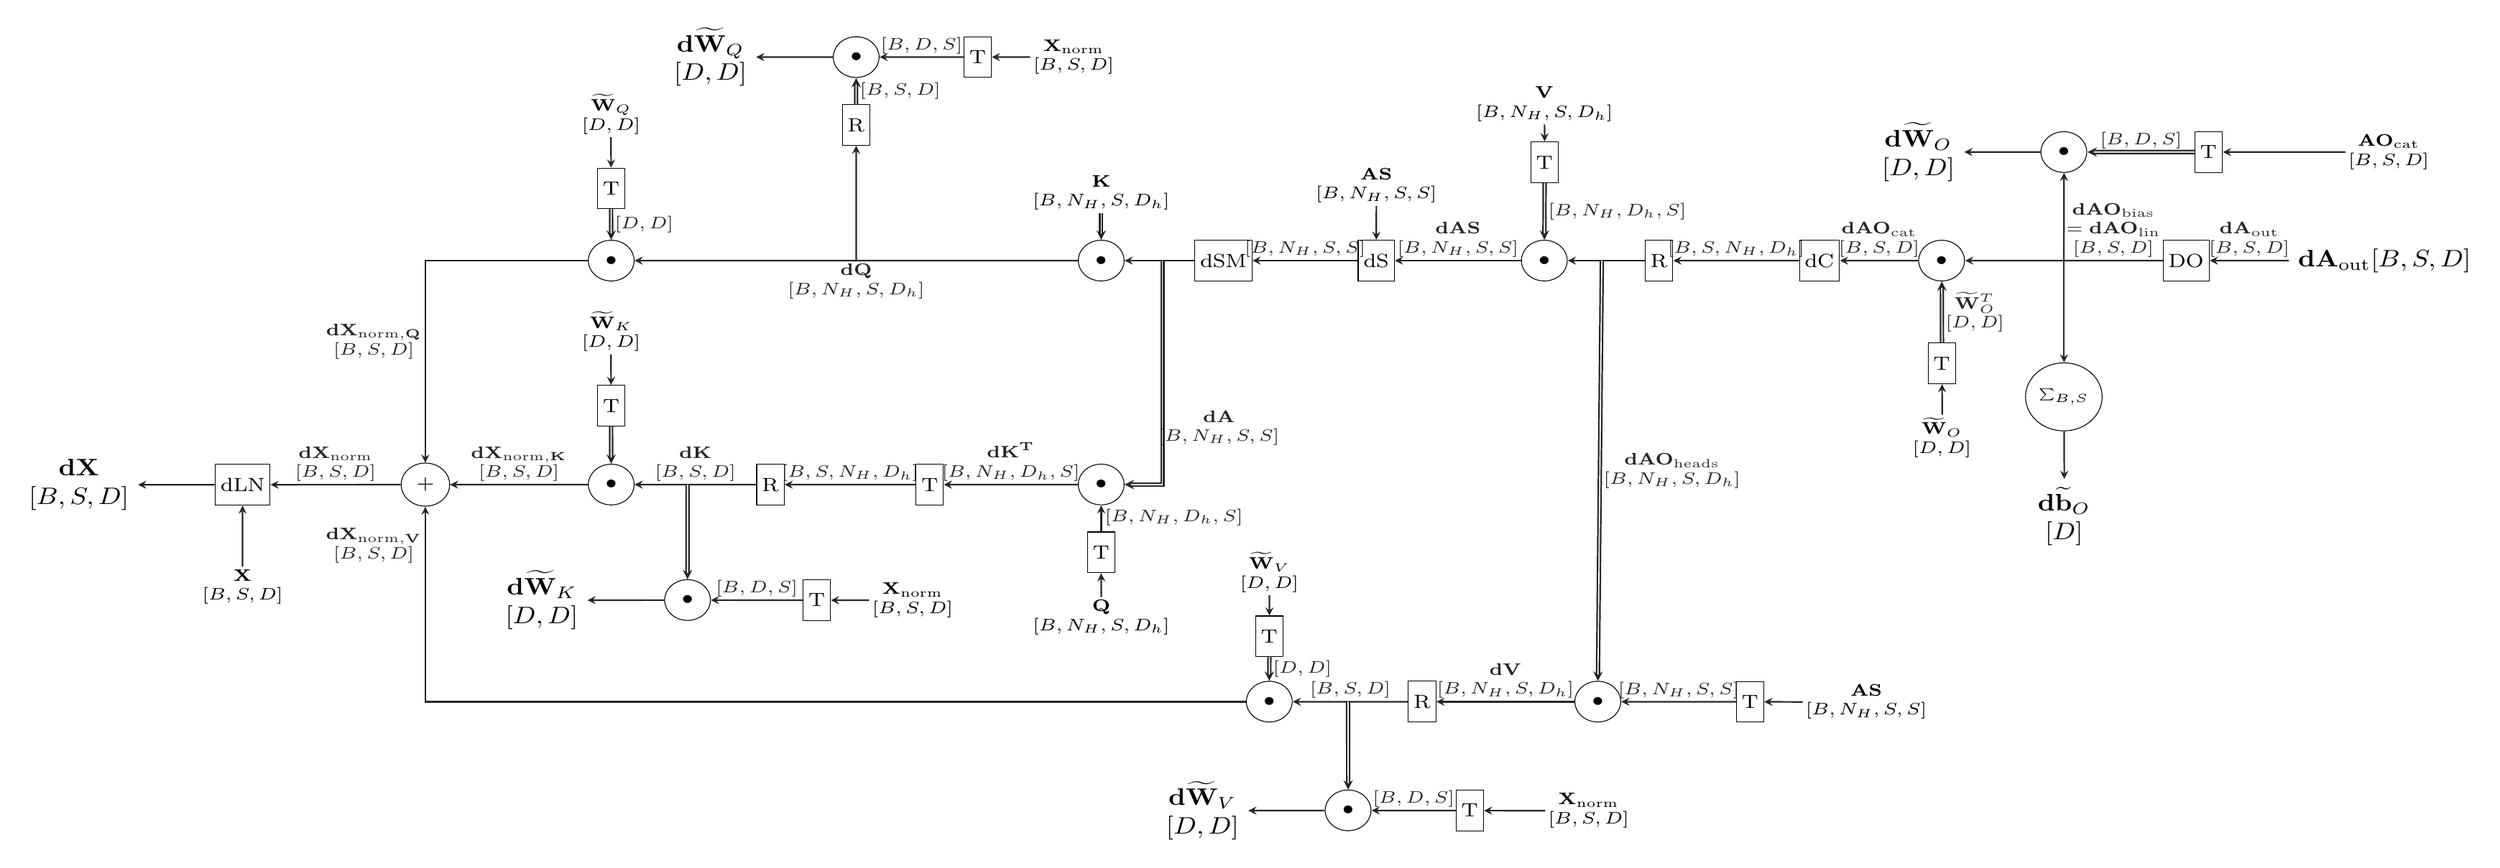
\begin{tikzpicture}[
  every node/.style={transform shape},
  >=stealth,
  auxnode/.style={draw, rectangle, fill=white, minimum height=6mm, inner sep=2pt, font=\footnotesize, align=center},
  mulnode/.style={draw, circle, fill=white, minimum size=6mm, font=\footnotesize, align=center},
  addnode/.style={draw, circle, fill=white, minimum size=6mm, font=\footnotesize, align=center},
  sumnode/.style={draw, circle, fill=white, minimum size=6mm, font=\tiny, align=center},
  flow/.style={->, thick, black!85},
  flow2/.style={->, double, thick, black!85},
  dimlabel/.style={font=\scriptsize, inner sep=1pt, align=center},
  gradflow/.style={->, thick, black!85},
  gradweight/.style={->, thick, black!85}
]

\begin{scope}[xscale=1.35, yscale=1.2]

\def\yoffset{-1.0}
\def\dVXyoffset{-6.5}

\coordinate (Grad_Aout_B) at (17.5, \yoffset);
\coordinate (dDrop_center) at (15.9, \yoffset);
\coordinate (ProjGradSplit) at (14.3, \yoffset);
\coordinate (dOProj_center) at (12.7, \yoffset);
\coordinate (C_center) at (11.1, \yoffset);
\coordinate (R_center) at (9.0, \yoffset);
\coordinate (dPV_AS_calc_center) at (7.5, \yoffset);
\coordinate (dSoft_center) at (5.3, \yoffset);
\coordinate (dSM_calc_center) at (3.3, \yoffset);
\coordinate (dV_calc_center) at (8.2, \dVXyoffset+\yoffset);
\coordinate (R_V_bwd_center) at (5.9, \dVXyoffset+\yoffset);
\coordinate (dVX_calc_center) at (3.9, \dVXyoffset+\yoffset);
\coordinate (dQK_calc_Q_center) at (1.7, \yoffset);
\coordinate (dQK_calc_K_center) at (1.7, -3.3+\yoffset);
\coordinate (K_BWD_input_center) at (1.7, 1.0+\yoffset);
\coordinate (T_Q_bwd_center) at (1.7, -4.3+\yoffset);

% \node[font=\Large\bfseries] at (8, 4.6+\yoffset) {Multi-Head Attention Backward Pass};

\node (Grad_Aout_B) at (18.5, \yoffset) {$\mathbf{dA}_{\text{out}}$\\$[B,S,D]$};
\node[auxnode] (DO) at (dDrop_center) {DO};
\node[mulnode] (dOProj) at (dOProj_center) {$\bullet$};

\node[auxnode] (T_WO) [below=0.9cm of dOProj] {T};
\node[dimlabel] (WO_BWD) [below=0.45cm of T_WO] {$\widetilde{\mathbf{W}}_{O}$\\$[D,D]$};

\node[mulnode] (dWO_calc) at ($(ProjGradSplit)+(0, 1.6)$) {$\bullet$};
\node[align=center, left=1.0cm of dWO_calc]
  (dWO_GRAD) {$\mathbf{d}\widetilde{\mathbf{W}}_{O}$\\$[D,D]$};
\node[auxnode] (T_AO_in) [right=1.4cm of dWO_calc] {T};
\node[dimlabel] (AO_in_local_label) [right=1.6cm of T_AO_in] {$\mathbf{AO}_{\text{cat}}$\\$[B,S,D]$};

\node[auxnode] (C) at (C_center) {dC};
\node[auxnode] (R) at (R_center) {R};

\node[mulnode] (dPV_AS_calc) at (dPV_AS_calc_center) {$\bullet$};
\node[auxnode] (dSoft) at (dSoft_center) {dS};
\node[auxnode] (dSM_calc) at (dSM_calc_center) {dSM};

\node[mulnode] (dQK_calc_Q) at (dQK_calc_Q_center) {$\bullet$};
\node[mulnode] (dQX_proj_calc) [left=5.8cm of dQK_calc_Q] {$\bullet$};

\node[mulnode] (dQK_calc_K) at (dQK_calc_K_center) {$\bullet$};
\node[mulnode] (dKX_proj_calc) [left=5.8cm of dQK_calc_K] {$\bullet$};

\node[dimlabel] (K_BWD_input) at (K_BWD_input_center) {$\mathbf{K}$\\$[B,N_H,S,D_h]$};
\node[auxnode] (T_Q_bwd) at (T_Q_bwd_center) {T};
\node[dimlabel] (Q_BWD_input) [below=0.35cm of T_Q_bwd] {$\mathbf{Q}$\\$[B,N_H,S,D_h]$};

\node[dimlabel] (V_FWD) [above=1.7cm of dPV_AS_calc] {$\mathbf{V}$\\$[B,N_H,S,D_h]$};
\node[auxnode] (T_V_bwd) [below=0.25cm of V_FWD] {T};

\node[mulnode] (dV_calc) at (dV_calc_center) {$\bullet$};
\node[auxnode] (T_AS_bwd) [right=1.5cm of dV_calc] {T};
\node[dimlabel] (AS_BWD_for_V) [right=0.5cm of T_AS_bwd] {$\mathbf{AS}$\\$[B,N_H,S,S]$};

\node[auxnode] (R_V_bwd) at (R_V_bwd_center) {R};
\node[mulnode] (dVX_calc) at (dVX_calc_center) {$\bullet$};

\node[auxnode] (T_WV) [above=0.35cm of dVX_calc] {T};
\node[dimlabel] (WV_BWD) [above=0.3cm of T_WV] {$\widetilde{\mathbf{W}}_{V}$\\$[D,D]$};

\node[sumnode] (Sum_dBO) [below=1.5cm of ProjGradSplit] {$\sum_{B, S}$};
\node (dBO) [align=center, below=0.7cm of Sum_dBO] {$\mathbf{d}\widetilde{\mathbf{b}}_{O}$\\$[D]$};

\draw[gradflow] (Grad_Aout_B) -- (DO)
  node[dimlabel, midway, above]{$\mathbf{dA}_{\text{out}}$\\$[B,S,D]$};

\draw[gradflow] (DO) -- (dOProj)
  node[dimlabel, pos=0.25, above]{$\mathbf{dAO}_{\text{bias}}$\\$=\mathbf{dAO}_{\text{lin}}$\\$[B,S,D]$};

\draw[gradflow] (ProjGradSplit) -- (dWO_calc.south);
\draw[gradflow] (ProjGradSplit) -- ([yshift=-0.75cm]ProjGradSplit) -| (Sum_dBO.north);

\draw[gradflow] (dOProj) -- (C)
  node[dimlabel, midway, above]{$\mathbf{dAO}_{\text{cat}}$\\$[B,S,D]$};
\draw[gradflow] (C) -- (R)
  node[dimlabel, midway, above]{$[B,S,N_H,D_h]$};

\coordinate (R_split_point) at ($(dPV_AS_calc)!0.5!(R)$);
\draw[gradflow] (R.west) -- (dPV_AS_calc.east);
\draw[flow2] (R_split_point) -- (dV_calc.north)
  node[dimlabel, midway, right]{$\mathbf{dAO}_{\text{heads}}$\\$[B,N_H,S,D_h]$};

\draw[gradflow] (V_FWD.south) -- (T_V_bwd.north);
\draw[flow2] (T_V_bwd.south) -- (dPV_AS_calc.north)
  node[dimlabel, midway, right]{$[B,N_H,D_h,S]$};
\draw[gradflow] (dPV_AS_calc.west) -- (dSoft.east)
  node[dimlabel, midway, above]{$\mathbf{dAS}$\\$[B,N_H,S,S]$};

\node (AS_BWD_dS) [dimlabel, above=0.5cm of dSoft] {$\mathbf{AS}$\\$[B,N_H,S,S]$};
\draw[gradflow] (AS_BWD_dS.south) -- (dSoft.north);
\draw[gradflow] (dSoft.west) -- (dSM_calc.east)
  node[dimlabel, midway, above]{$[B,N_H,S,S]$};

\coordinate (dA_Split_X) at ($(dSM_calc_center)!0.5!(dQK_calc_Q_center)$);
\coordinate (dA_Split) at (dA_Split_X |- dQK_calc_Q.east);
\draw[gradflow] (dSM_calc.west) -- (dQK_calc_Q.east);
\draw[flow2] (dA_Split) -- (dA_Split |- dQK_calc_K.east) -- (dQK_calc_K.east)
  node[dimlabel, pos=-1.5, above, yshift=15]{$\mathbf{dA}$\\$[B,N_H,S,S]$};

\draw[flow2] (K_BWD_input.south) -- (dQK_calc_Q.north);
\draw[gradweight] (dQK_calc_Q) -- (dQX_proj_calc)
  node[dimlabel, midway, below]{$\mathbf{dQ}$\\$[B,N_H,S,D_h]$};

\node[auxnode] (T_WQ_bwd) [above=0.45cm of dQX_proj_calc] {T};
\node[dimlabel] (WQ_bwd) [above=0.45cm of T_WQ_bwd] {$\widetilde{\mathbf{W}}_{Q}$\\$[D,D]$};
\draw[flow] (WQ_bwd) -- (T_WQ_bwd);
\draw[flow2] (T_WQ_bwd.south) -- (dQX_proj_calc.north)
  node[dimlabel, midway, right]{$[D,D]$};

\draw[flow] (Q_BWD_input.north) -- (T_Q_bwd.south);
\draw[flow] (T_Q_bwd.north) -- (dQK_calc_K.south)
  node[dimlabel, pos=0.55, right]{$[B,N_H,D_h,S]$};

\node[auxnode] (T_dK) at ($(dQK_calc_K)!0.35!(dKX_proj_calc)$) {T};
\node[auxnode] (R_dK_mid) at ($(T_dK)!0.5!(dKX_proj_calc)$) {R};

\draw[gradweight] (dQK_calc_K) -- (T_dK)
  node[dimlabel, midway, above]{$\mathbf{dK^T}$\\$[B,N_H,D_h,S]$};
\draw[gradweight] (T_dK) -- (R_dK_mid)
  node[dimlabel, midway, above]{$[B,S,N_H,D_h]$};
\draw[gradweight] (R_dK_mid) -- (dKX_proj_calc)
  node[dimlabel, midway, above]{$\mathbf{dK}$\\$[B,S,D]$};

\node[auxnode] (T_WK_bwd) [above=0.55cm of dKX_proj_calc] {T};
\node[dimlabel] (WK_bwd) [above=0.45cm of T_WK_bwd] {$\widetilde{\mathbf{W}}_{K}$\\$[D,D]$};
\draw[gradflow] (WK_bwd) -- (T_WK_bwd);
\draw[flow2] (T_WK_bwd.south) -- (dKX_proj_calc.north);

\draw[gradflow] (AS_BWD_for_V.west) -- (T_AS_bwd.east);
\draw[gradflow] (T_AS_bwd.west) -- (dV_calc.east)
  node[dimlabel, midway, above]{$[B,N_H,S,S]$};
\draw[gradflow] (dV_calc.west) -- (R_V_bwd.east)
  node[dimlabel, midway, above]{$\mathbf{dV}$\\$[B,N_H,S,D_h]$};
\draw[gradflow] (R_V_bwd) -- (dVX_calc.east)
  node[dimlabel, midway, above]{$[B,S,D]$};

\draw[gradflow] (WV_BWD) -- (T_WV);
\draw[flow2] (T_WV) -- (dVX_calc.north)
  node[dimlabel, midway, right]{$[D,D]$};

\node[addnode] (Sum_dXnorm) [left=1.8cm of dKX_proj_calc] {$+$};

\draw[gradweight] (dQX_proj_calc.west) -| node[dimlabel, pos=0.7, left]{$\mathbf{dX}_{\text{norm},\mathbf{Q}}$\\$[B,S,D]$} (Sum_dXnorm.north);
\draw[gradweight] (dKX_proj_calc.west) -- node[dimlabel, midway, above]{$\mathbf{dX}_{\text{norm},\mathbf{K}}$\\$[B,S,D]$} (Sum_dXnorm.east);
\draw[gradweight] (dVX_calc.west) -| node[dimlabel, pos=0.9, left]{$\mathbf{dX}_{\text{norm},\mathbf{V}}$\\$[B,S,D]$} (Sum_dXnorm.south);

\coordinate (dV_branch) at ($(R_V_bwd.west)!0.52!(dVX_calc.east)$);
\node[mulnode] (dWV_mul) at ($(dV_branch)+(0,-1.6cm)$) {$\bullet$};
\draw[flow2] (dV_branch) -- (dWV_mul.north);

\node[auxnode] (T_Xnorm) [right=1.1cm of dWV_mul] {T};
\node[dimlabel] (Xnorm_local) [right=0.8cm of T_Xnorm] {$\mathbf{X}_{\text{norm}}$\\$[B,S,D]$};
\draw[gradflow] (Xnorm_local) -- (T_Xnorm);
\draw[gradflow] (T_Xnorm.west) -- (dWV_mul.east)
  node[dimlabel, midway, above]{$[B,D,S]$};
\node (dWV_out) [align=center, left=1.0cm of dWV_mul] {$\mathbf{d}\widetilde{\mathbf{W}}_{V}$\\$[D,D]$};
\draw[gradweight] (dWV_mul.west) -- (dWV_out);

\coordinate (dQ_branch) at ($(dQK_calc_Q.east)!0.50!(dQX_proj_calc.west)$);
\node[mulnode] (dWQ_mul) at ($(dQ_branch)+(0,3.0cm)$) {$\bullet$};
\node[auxnode] (R_dQ_for_WQ) at ($(dWQ_mul)+(0,-1.0cm)$) {R};
\draw[gradflow]  (dQ_branch) -- (R_dQ_for_WQ.south);
\draw[flow2] (R_dQ_for_WQ.north) -- (dWQ_mul.south)
  node[dimlabel, midway, right]{$[B,S,D]$};

\node[auxnode] (T_XnormQ) [right=1.1cm of dWQ_mul] {T};
\node[dimlabel] (Xnorm_localQ) [right=0.5cm of T_XnormQ] {$\mathbf{X}_{\text{norm}}$\\$[B,S,D]$};
\draw[gradflow] (Xnorm_localQ) -- (T_XnormQ);
\draw[gradflow] (T_XnormQ.west) -- (dWQ_mul.east)
  node[dimlabel, midway, above]{$[B,D,S]$};
\node (dWQ_out) [align=center, left=1.0cm of dWQ_mul] {$\mathbf{d}\widetilde{\mathbf{W}}_{Q}$\\$[D,D]$};
\draw[gradweight] (dWQ_mul.west) -- (dWQ_out);

\coordinate (dK_branch) at ($(R_dK_mid)!0.52!(dKX_proj_calc)$);
\node[mulnode] (dWK_mul) at ($(dK_branch)+(0,-1.7cm)$) {$\bullet$};
\draw[flow2]  (dK_branch) -- (dWK_mul.north);

\node[auxnode] (T_XnormK) [right=1.2cm of dWK_mul] {T};
\node[dimlabel, right=0.5cm of T_XnormK] (Xnorm_localK) {$\mathbf{X}_{\text{norm}}$\\$[B,S,D]$};
\draw[gradflow] (Xnorm_localK) -- (T_XnormK);
\draw[gradflow] (T_XnormK.west) -- (dWK_mul.east)
  node[dimlabel, midway, above]{$[B,D,S]$};
\node (dWK_out) [align=center, left=1.0cm of dWK_mul] {$\mathbf{d}\widetilde{\mathbf{W}}_{K}$\\$[D,D]$};
\draw[gradweight] (dWK_mul.west) -- (dWK_out);

\draw[gradweight] (Sum_dBO) -- (dBO);

\draw[gradflow] (WO_BWD) -- (T_WO);
\draw[flow2] (T_WO) -- (dOProj)
  node[dimlabel, midway, right]{$\widetilde{\mathbf{W}}_{O}^{T}$\\$[D,D]$};
\draw[gradflow] (AO_in_local_label) -- (T_AO_in);
\draw[flow2] (T_AO_in) -- (dWO_calc.east)
  node[dimlabel, midway, above]{$[B,D,S]$};
\draw[gradweight] (dWO_calc) -- (dWO_GRAD);

\node[auxnode] (dLN) [left=1.7cm of Sum_dXnorm] {dLN};
\draw[gradweight] (Sum_dXnorm.west) -- node[dimlabel, midway, above]
  {$\mathbf{dX}_{\text{norm}}$\\$[B,S,D]$} (dLN.east);

\node (dX_OUT) [align=center, left=1.0cm of dLN] {$\mathbf{dX}$\\$[B,S,D]$};
\draw[gradweight] (dLN.west) -- (dX_OUT);

\node[dimlabel] (LNCache) [below=0.9cm of dLN] {$\mathbf{X}$\\$[B,S,D]$};
\draw[gradflow] (LNCache.north) -- (dLN.south);

\end{scope}
\end{tikzpicture}
}

\end{landscape}
\clearpage

% ------------------------ 4.3 MLP / FFN Block ------------------------
\subsection{Feed-Forward Network (MLP / FFN)}

\subsubsection{Forward Pass}
\resizebox{\linewidth}{!}{%
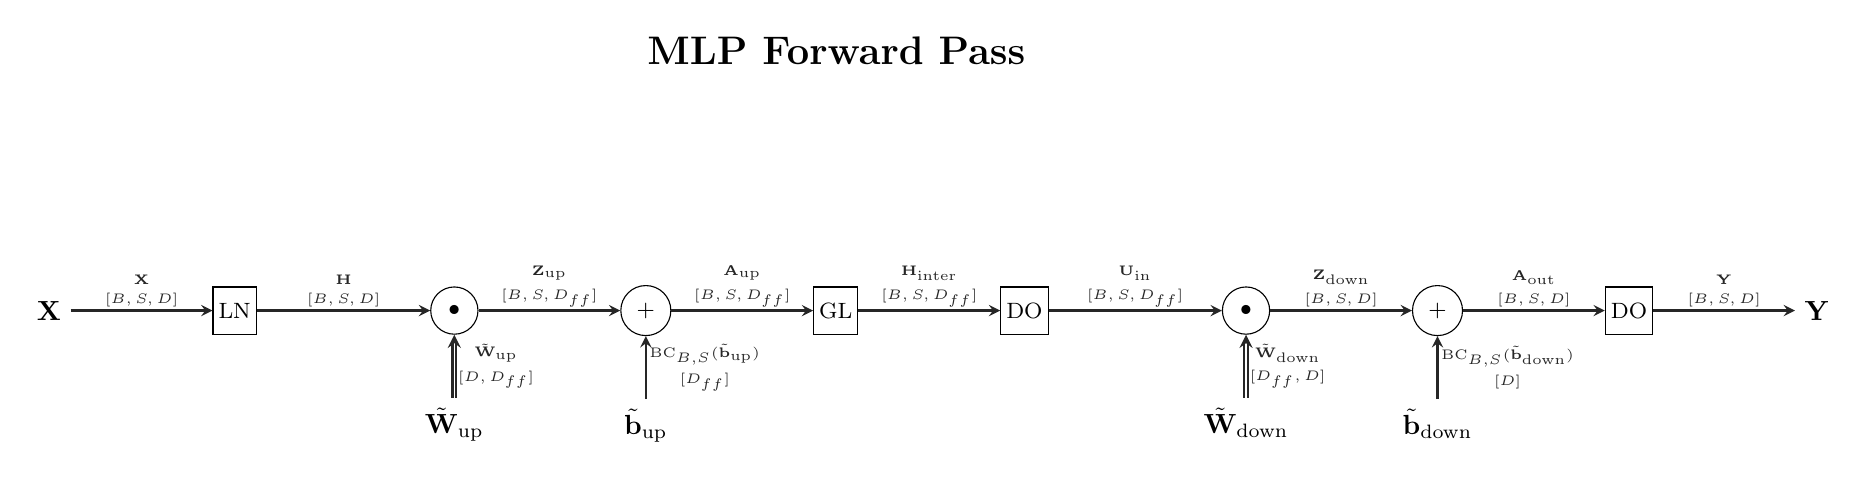
\begin{tikzpicture}[
    >=stealth,
    auxnode/.style={draw, rectangle, fill=white, minimum height=6mm, inner sep=2pt, font=\footnotesize, align=center},
    mulnode/.style={draw, circle, fill=white, minimum size=6mm, font=\footnotesize, align=center},
    addnode/.style={draw, circle, fill=white, minimum size=6mm, font=\footnotesize, align=center},
    sumnode/.style={draw, circle, fill=white, minimum size=6mm, font=\tiny, align=center},
    flow/.style={->, thick, black!85},
    flow2/.style={double, ->, thick, black!85},
    dimlabel/.style={font=\tiny, inner sep=1pt, align=center}
]
    \node[font=\Large\bfseries] at (10, 2.8) {MLP Forward Pass};

    \pgfmathsetmacro{\verticaloffset}{-0.5}

    \node            (MIn)   at (0,\verticaloffset) {$\mathbf{X}$};
    \node[auxnode]   (LN2)   [right=1.8cm of MIn] {LN};
    \node[mulnode]   (L1Mul) [right=2.2cm of LN2] {$\bullet$};
    \node            (Wup)   [below=0.8cm of L1Mul] {$\tilde{\mathbf{W}}_{\text{up}}$};
    \node[addnode]   (AddB1) [right=1.8cm of L1Mul] {+};
    \node            (Bup)   [below=0.8cm of AddB1] {$\tilde{\mathbf{b}}_{\text{up}}$};
    \node[auxnode]   (Act)   [right=1.8cm of AddB1] {GL};
    \node[auxnode]   (Drop1) [right=1.8cm of Act] {DO};
    \node[mulnode]   (L2Mul) [right=2.2cm of Drop1] {$\bullet$};
    \node            (Wdown) [below=0.8cm of L2Mul] {$\tilde{\mathbf{W}}_{\text{down}}$};
    \node[addnode]   (AddB2) [right=1.8cm of L2Mul] {+};
    \node            (Bdown) [below=0.8cm of AddB2] {$\tilde{\mathbf{b}}_{\text{down}}$};
    \node[auxnode]   (Drop2) [right=1.8cm of AddB2] {DO};
    \node            (MOut)  [right=1.8cm of Drop2] {$\mathbf{Y}$};

    \draw[flow] (MIn) -- (LN2) node[dimlabel, midway, above]{\shortstack{$\mathbf{X}$\\$[B,S,D]$}};
    \draw[flow] (LN2) -- (L1Mul) node[dimlabel, midway, above]{\shortstack{$\mathbf{H}$\\$[B,S,D]$}};
    \draw[flow2] (Wup) -- (L1Mul) node[dimlabel, midway, right]{\shortstack{$\tilde{\mathbf{W}}_{\text{up}}$\\$[D, D_{ff}]$}};
    \draw[flow] (L1Mul) -- (AddB1) node[dimlabel, midway, above]{\shortstack{$\mathbf{Z}_{\text{up}}$\\$[B,S,D_{ff}]$}};
    \draw[flow] (Bup) -- (AddB1) node[dimlabel, midway, right]{\shortstack{$\mathrm{BC}_{B,S}(\tilde{\mathbf{b}}_{\text{up}})$\\$[D_{ff}]$}};
    \draw[flow] (AddB1) -- (Act) node[dimlabel, midway, above]{\shortstack{$\mathbf{A}_{\text{up}}$\\$[B,S,D_{ff}]$}};
    \draw[flow] (Act) -- (Drop1) node[dimlabel, midway, above]{\shortstack{$\mathbf{H}_{\text{inter}}$\\$[B,S,D_{ff}]$}};
    \draw[flow] (Drop1) -- (L2Mul) node[dimlabel, midway, above]{\shortstack{$\mathbf{U}_{\text{in}}$\\$[B,S,D_{ff}]$}};
    \draw[flow2] (Wdown) -- (L2Mul) node[dimlabel, midway, right]{\shortstack{$\tilde{\mathbf{W}}_{\text{down}}$\\$[D_{ff}, D]$}};
    \draw[flow] (L2Mul) -- (AddB2) node[dimlabel, midway, above]{\shortstack{$\mathbf{Z}_{\text{down}}$\\$[B,S,D]$}};
    \draw[flow] (Bdown) -- (AddB2) node[dimlabel, midway, right]{\shortstack{$\mathrm{BC}_{B,S}(\tilde{\mathbf{b}}_{\text{down}})$\\$[D]$}};
    \draw[flow] (AddB2) -- (Drop2) node[dimlabel, midway, above]{\shortstack{$\mathbf{A}_{\text{out}}$\\$[B,S,D]$}};
    \draw[flow] (Drop2) -- (MOut) node[dimlabel, midway, above]{\shortstack{$\mathbf{Y}$\\$[B,S,D]$}};

\end{tikzpicture}%
}


\clearpage

\subsubsection{Backward Pass}
\noindent
\resizebox{\linewidth}{!}{%
\begin{tikzpicture}[
    >=stealth,
    auxnode/.style={draw, rectangle, fill=white, minimum height=6mm, inner sep=2pt, font=\footnotesize, align=center},
    mulnode/.style={draw, circle, fill=white, minimum size=6mm, font=\footnotesize, align=center},
    addnode/.style={draw, circle, fill=white, minimum size=6mm, font=\footnotesize, align=center},
    sumnode/.style={draw, circle, fill=white, minimum size=6mm, font=\tiny, align=center},
    flow_rev/.style={<-, thick, black!85},
    flow_dw/.style={->, thick, black!85},
    flow_act/.style={double, ->, thick, black!85},
    dimlabel/.style={font=\tiny, inner sep=1pt, align=center},
    gradlabel/.style={font=\tiny\bfseries, inner sep=1pt, align=center}
]
    \node[font=\Large\bfseries] at (5, 10) {MLP Backward Pass};

    \pgfmathsetmacro{\backwardoffset}{0.0}

    \node (d_MOut) at (12.6, \backwardoffset) {$\mathrm{d}\mathbf{Y}$};
    \node[auxnode] (d_Drop2) [left=1.8cm of d_MOut] {dDO};
    \draw[flow_rev] (d_Drop2) -- (d_MOut)
      node[dimlabel, midway, below]{\shortstack{$\mathrm{d}\mathbf{Y}$\\$[B,S,D]$}};

    \coordinate (split2) at ($(d_Drop2.west) + (-1.5cm, 0)$);
    \coordinate (branch_dUproj) at ($(split2) + (-1.2cm, 0)$);

    \node[sumnode] (d_SumB2) [above=0.8cm of split2] {$\sum_{B, S}$};
    \node (d_Bdown) [above=0.8cm of d_SumB2] {$\mathrm{d}\tilde{\mathbf{b}}_{\text{down}}$};
    \draw[flow_dw] (d_SumB2) -- (d_Bdown) node[dimlabel, midway, right]{$[D]$};

    \draw[flow_rev] (split2) -- (d_Drop2);
    \draw[flow_rev] (d_SumB2) -- (split2);

    \node[mulnode] (d_L2Mul_in) [left=2.2cm of split2] {$\bullet$};
    \draw[flow_rev] (d_L2Mul_in) -- (d_Drop2)
      node[gradlabel, midway, below]{\shortstack{$\mathrm{d}\mathbf{Z}_{\text{down}}=\mathrm{d}\mathbf{A}_{\text{out}}$\\$[B,S,D]$}};

    \node (W_down_T) [below=1.8cm of d_L2Mul_in] {$\tilde{\mathbf{W}}_{\text{down}}^{T}$};
    \draw[flow_act] (W_down_T.north) -- (d_L2Mul_in)
      node[dimlabel, midway, right]{$[D, D_{ff}]$};

    \coordinate (L2Mul_w_y) at ($(d_L2Mul_in) + (0, 3.5cm)$);
    \node[mulnode] (d_L2Mul_w) at (L2Mul_w_y) {$\bullet$};
    \node (d_Wdown) [above=0.8cm of d_L2Mul_w] {$\mathrm{d}\tilde{\mathbf{W}}_{\text{down}}$};
    \draw[flow_dw] (d_L2Mul_w) -- (d_Wdown) node[dimlabel, midway, right]{$[D_{ff}, D]$};

    \draw[flow_act] (branch_dUproj.north) |- (d_L2Mul_w.east);

    \node[auxnode] (Uin_T) at ($(d_L2Mul_w.west) + (-1.5cm, 0)$) {T};
    \draw[flow_dw] (Uin_T) -- (d_L2Mul_w)
      node[dimlabel, midway, below]{\shortstack{$\mathbf{U}_{\text{in}}^T$\\$[B, D_{ff}, S]$}};
    \node (Uin_aux) [left=1.8cm of Uin_T] {$\mathbf{U}_{\text{in}}$};
    \draw[flow_dw] (Uin_aux) -- (Uin_T) node[dimlabel, midway, above]{\shortstack{$[B,S,D_{ff}]$}};

    \node[auxnode] (d_Drop1) [left=1.8cm of d_L2Mul_in] {dDO};
    \draw[flow_rev] (d_Drop1) -- (d_L2Mul_in)
      node[dimlabel, midway, below]{\shortstack{$\mathrm{d}\mathbf{U}_{\text{in}}$\\$[B,S,D_{ff}]$}};

    \node[auxnode] (d_Act) [left=1.8cm of d_Drop1] {dGL};
    \draw[flow_rev] (d_Act) -- (d_Drop1)
      node[dimlabel, midway, below]{\shortstack{$\mathrm{d}\mathbf{H}_{\text{inter}}$\\$[B,S,D_{ff}]$}};

    \coordinate (split1) at ($(d_Act.west) + (-1.5cm, 0)$);
    \coordinate (branch_dHpre) at ($(split1) + (-1.2cm, 0)$);

    \node[sumnode] (d_SumB1) [above=0.8cm of split1] {$\sum_{B, S}$};
    \node (d_Bup) [above=0.8cm of d_SumB1] {$\mathrm{d}\tilde{\mathbf{b}}_{\text{up}}$};
    \draw[flow_dw] (d_SumB1) -- (d_Bup) node[dimlabel, midway, right]{$[D_{ff}]$};

    \draw[flow_rev] (split1) -- (d_Act);
    \draw[flow_rev] (d_SumB1) -- (split1);

    \node[mulnode] (d_L1Mul_in) [left=2.2cm of split1] {$\bullet$};
    \draw[flow_rev] (d_L1Mul_in) -- (d_Act)
      node[gradlabel, midway, below]{\shortstack{$\mathrm{d}\mathbf{Z}_{\text{up}}=\mathrm{d}\mathbf{A}_{\text{up}}$\\$[B,S,D_{ff}]$}};

    \node (W_up_T) [below=1.8cm of d_L1Mul_in] {$\tilde{\mathbf{W}}_{\text{up}}^{T}$};
    \draw[flow_act] (W_up_T.north) -- (d_L1Mul_in)
      node[dimlabel, midway, right]{$[D_{ff}, D]$};

    \coordinate (L1Mul_w_y) at ($(d_L1Mul_in) + (0, 3.5cm)$);
    \node[mulnode] (d_L1Mul_w) at (L1Mul_w_y) {$\bullet$};
    \node (d_Wup) [above=0.8cm of d_L1Mul_w] {$\mathrm{d}\tilde{\mathbf{W}}_{\text{up}}$};
    \draw[flow_dw] (d_L1Mul_w) -- (d_Wup) node[dimlabel, midway, right]{$[D, D_{ff}]$};

    \draw[flow_act] (branch_dHpre.north) |- (d_L1Mul_w.east);

    \node[auxnode] (Znorm_T) at ($(d_L1Mul_w.west) + (-1.5cm, 0)$) {T};
    \draw[flow_dw] (Znorm_T) -- (d_L1Mul_w)
      node[dimlabel, midway, below]{\shortstack{$\mathbf{H}^T$\\$[B, D, S]$}};
    \node (Znorm_aux) [left=1.8cm of Znorm_T] {$\mathbf{H}$};
    \draw[flow_dw] (Znorm_aux) -- (Znorm_T) node[dimlabel, midway, above]{\shortstack{$[B,S,D]$}};

    \node[auxnode] (d_LN2) [left=1.8cm of d_L1Mul_in] {dLN};
    \draw[flow_rev] (d_LN2) -- (d_L1Mul_in)
      node[dimlabel, midway, below]{\shortstack{$\mathrm{d}\mathbf{H}$\\$[B,S,D]$}};

    \node (d_MIn) [left=1.8cm of d_LN2] {$\mathrm{d}\mathbf{X}$};
    \draw[flow_rev] (d_MIn) -- (d_LN2)
      node[dimlabel, midway, below]{\shortstack{$\mathrm{d}\mathbf{X}$\\$[B,S,D]$}};
\end{tikzpicture}%
}


\clearpage

% ------------------------ 4.4 Output Projection & Loss ---------------
\subsection{Output Projection and Loss}

\subsubsection{Forward Pass (Logits, Softmax, Loss)}

\noindent
\resizebox{\linewidth}{!}{%
\begin{tikzpicture}[
  >=stealth,
  auxnode/.style={draw, rectangle, fill=white, minimum height=6mm, inner sep=2pt, font=\footnotesize, align=center},
  mulnode/.style={draw, circle, fill=white, minimum size=6mm, font=\footnotesize, align=center},
  addnode/.style={draw, circle, fill=white, minimum size=6mm, font=\footnotesize, align=center},
  sumnode/.style={draw, circle, fill=white, minimum size=6mm, font=\tiny, align=center},
  flow/.style={->, thick, black!85},
  flow2/.style={double, ->, thick, black!85},
  dimlabel/.style={font=\tiny, inner sep=1pt, align=center}
]

% From Transformer output
\node            (H)     at (0,-2) {$\mathbf{A}_{\text{out}}$};

% LM head
\node[mulnode]   (LMmul) [right=2.2cm of H] {$\bullet$};
\node            (Wlm)   [align=center, below=0.9cm of LMmul] {$\widetilde{\mathbf{W}}_{\text{lm}}$\\$=\mathbf{E}^{T}$};
\node[addnode]   (AddB)  [right=1.8cm of LMmul] {+};
\node            (blm)   [below=0.9cm of AddB] {$\widetilde{\mathbf{b}}_{\text{lm}}$};

% Softmax → Prob
\node[auxnode]   (SM)    [right=1.8cm of AddB] {S};

\node[auxnode] (ARG)  [right=4.0cm of SM] {ARG};
% Midpoint of SM→P edge (for CE tap)
\coordinate (MidSP) at ($(SM)!0.5!(ARG)$);

% CE node placed below the SM→P edge
\node[auxnode]   (CE)    [below=1.6cm of MidSP] {CE};
\node            (Y)     [right=0.9cm of CE] {$\mathbf{Y_\text{targets}}$};
\node            (Loss)  [align=center, below=1.8cm of CE] {$\mathcal{L}$\\ (mean over $B,S$)};

% Flows
\draw[flow]  (H) -- (LMmul) node[dimlabel, midway, above]{\shortstack{$[B,S,D]$}};
\draw[flow2] (Wlm) -- (LMmul) node[dimlabel, midway, right]{\shortstack{$[D,V]$}};
\draw[flow]  (LMmul) -- (AddB) node[dimlabel, midway, above]{\shortstack{$\mathbf{Z}_{\text{lin}}$\\$[B,S,V]$}};
\draw[flow]  (blm) -- (AddB)   node[dimlabel, midway, right]{\shortstack{$\text{BC}_{B,S}(\widetilde{\mathbf{b}}_{\text{lm}})$\\$[V]$}};
\draw[flow]  (AddB) -- (SM)    node[dimlabel, midway, above]{\shortstack{\textbf{Z\textsubscript{bias}}\\ $[B,S,V]$}};

% Tap the SM→P edge downward into CE
\draw[flow]  (MidSP) -- (CE);
% Targets into CE
\draw[flow]  (Y) -- (CE)  node[dimlabel, midway, above]{\shortstack{targets\\$[B,S]$}};
% Loss goes WEST (left) from CE
\draw[flow]  (CE) -- (Loss);

\node (YhatG) [right=1.8cm of ARG] {$\hat{\mathbf{Y}}_{\text{greedy}}$};
\draw[flow] (SM) -- (ARG)
  node[dimlabel, pos=0.35, above]{\shortstack{$\mathbf{P}$\\$[B,S,V]$}};
\draw[flow] (ARG) -- (YhatG)
  node[dimlabel, midway, above]{\shortstack{token ids\\$[B,S]$}};

% Optional: top-k (or nucleus) sampling path
\node[auxnode] (TopK) [above=1.4cm of ARG] {TOP-$k$};
\node          (YhatS) [right=1.8cm of TopK] {$\hat{\mathbf{Y}}_{\text{sample}}$};
\draw[flow] (MidSP) |- (TopK);
\draw[flow] (TopK) -- (YhatS)
  node[dimlabel, midway, above]{\shortstack{token ids\\$[B,S]$}};

\node[font=\large\bfseries] at (9.2,1.8) {Token Generation \& Loss (Forward)};
\end{tikzpicture}%
}


\clearpage

\subsubsection{Backward Pass}
\noindent
\resizebox{0.8\linewidth}{!}{%
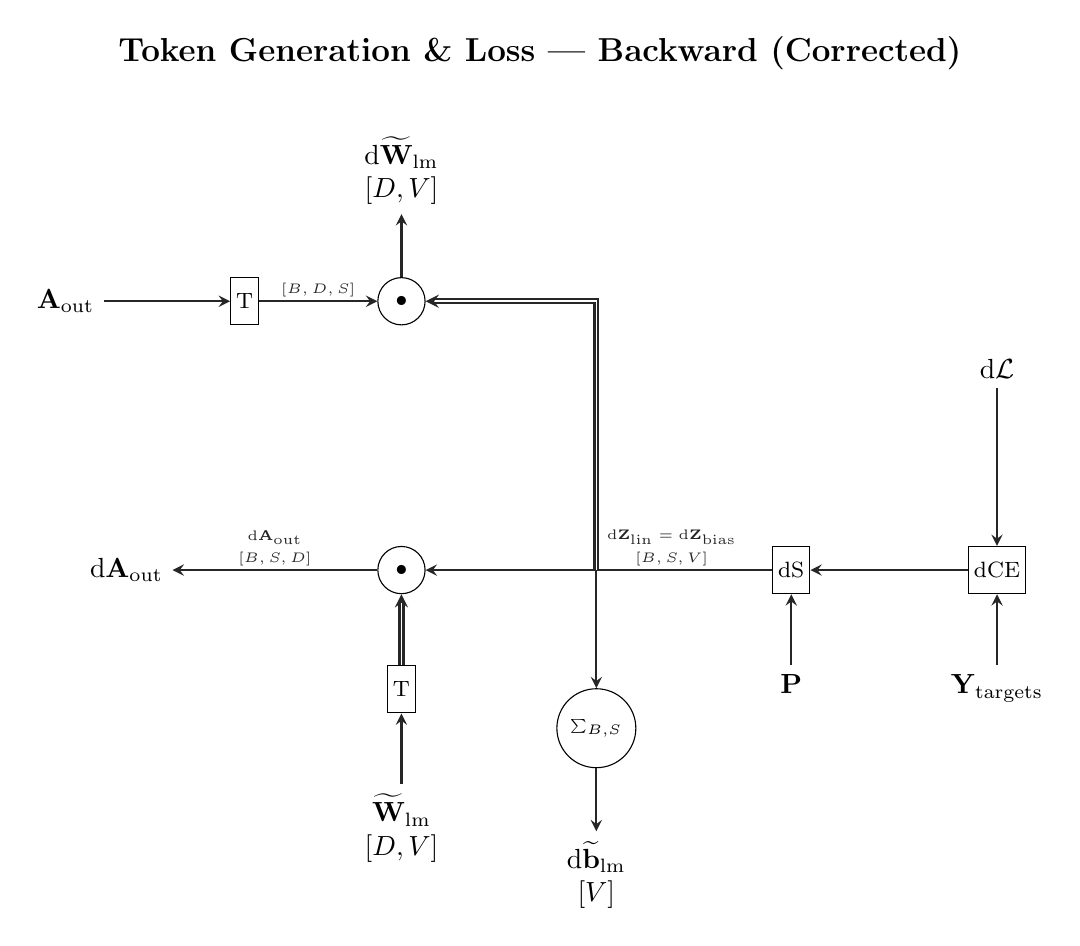
\begin{tikzpicture}[
  >=stealth,
  auxnode/.style={draw, rectangle, fill=white, minimum height=6mm, inner sep=2pt, font=\footnotesize, align=center},
  mulnode/.style={draw, circle, fill=white, minimum size=6mm, font=\footnotesize, align=center},
  addnode/.style={draw, circle, fill=white, minimum size=6mm, font=\footnotesize, align=center},
  sumnode/.style={draw, circle, fill=white, minimum size=6mm, font=\tiny, align=center},
  flow/.style={<-, thick, black!85},
  flow2/.style={double, <-, thick, black!85},
  fwd/.style={->, thick, black!85},
  gradflow/.style={->, thick, black!85},
  dimlabel/.style={font=\tiny, inner sep=1pt, align=center}
]

% Start from dL
\node           (dL)    at (18,0) {$\text{d}\mathcal{L}$};
\node[auxnode]  (dCE)   [below=2.0cm of dL] {dCE};
\node           (Y)     [below=0.9cm of dCE] {$\mathbf{Y_\text{targets}}$};

% Softmax backward
\node[auxnode]  (dS)   [left=2.0cm of dCE] {dS};
\node           (P)     [below=0.9cm of dS] {$\mathbf{P}$};

% Logits (Linear Projection) backprop node
\node[mulnode]  (backMul) [left=4.4cm of dS] {$\bullet$};
\node[auxnode]  (T_Wlm)   [below=0.9cm of backMul] {T};
\node           (Wlm)     [align=center, below=0.9cm of T_Wlm] {$\widetilde{\mathbf{W}}_{\text{lm}}$\\$[D,V]$};

\coordinate (B_split) at ($(backMul)!0.5!(dS)$);

% SUM node for Bias gradient
\node[sumnode]  (SumB) [below=1.5cm of B_split] {$\sum_{B,S}$};
\node           (db)   [align=center, below=0.8cm of SumB] {$\text{d}\widetilde{\mathbf{b}}_{\text{lm}}$\\$[V]$};

% dW calc
\node[mulnode]  (dWmul) [above=2.8cm of backMul] {$\bullet$};
\node[auxnode]  (TAout) [left=1.5cm of dWmul] {T};
\node           (Aout)  [left=1.6cm of TAout] {$\mathbf{A}_{\text{out}}$};
\node           (dW)    [align=center, above=0.8cm of dWmul] {$\text{d}\widetilde{\mathbf{W}}_{\text{lm}}$\\$[D,V]$};

% Back to Transformer
\node           (dH)    [left=2.6cm of backMul] {$\text{d}\mathbf{A}_{\text{out}}$};

% Flows
\draw[flow] (dCE) -- (dL);
\draw[fwd]  (Y) -- (dCE);
\draw[flow] (dS) -- (dCE);
\draw[fwd]  (P) -- (dS);

% Bias grad
\draw[gradflow] (B_split) -- (SumB.north);
\draw[gradflow] (SumB) -- (db);

% Linear projection backprop
\draw[flow] (backMul) -- (dS)
  node[dimlabel, pos=0.71, above]{\shortstack{$\text{d}\mathbf{Z}_{\text{lin}}=\text{d}\mathbf{Z}_{\text{bias}}$\\$[B,S,V]$}};
\draw[flow2] (backMul) -- (T_Wlm);
\draw[fwd]   (Wlm) -- (T_Wlm);
\draw[flow]  (dH) -- (backMul) node[dimlabel, midway, above]{\shortstack{$\text{d}\mathbf{A}_{\text{out}}$\\$[B,S,D]$}};

% dW calculation
\draw[gradflow] (dWmul) -- (dW);
\draw[fwd]  (Aout) -- (TAout);
\draw[fwd]  (TAout) -- (dWmul) node[dimlabel, midway, above]{\shortstack{$[B,D,S]$}};
\draw[flow2] (dWmul) -| (B_split);

\node[font=\large\bfseries, anchor=south]
  at ([yshift=6mm]current bounding box.north) {Token Generation \& Loss — Backward (Corrected)};
\end{tikzpicture}%
}


\clearpage

% ==========================================================
% 5. Tensor Parallelism (TP)
% ==========================================================
\section{Tensor Parallelism (TP)}

In tensor parallelism, weight matrices are partitioned across multiple
devices along certain dimensions. Each device computes on its own shard,
and collective operations (e.g., All-Reduce, All-Gather) synchronize
intermediate results.

\subsection{TP Overview and End-to-End Flow}
\resizebox{\linewidth}{!}{%
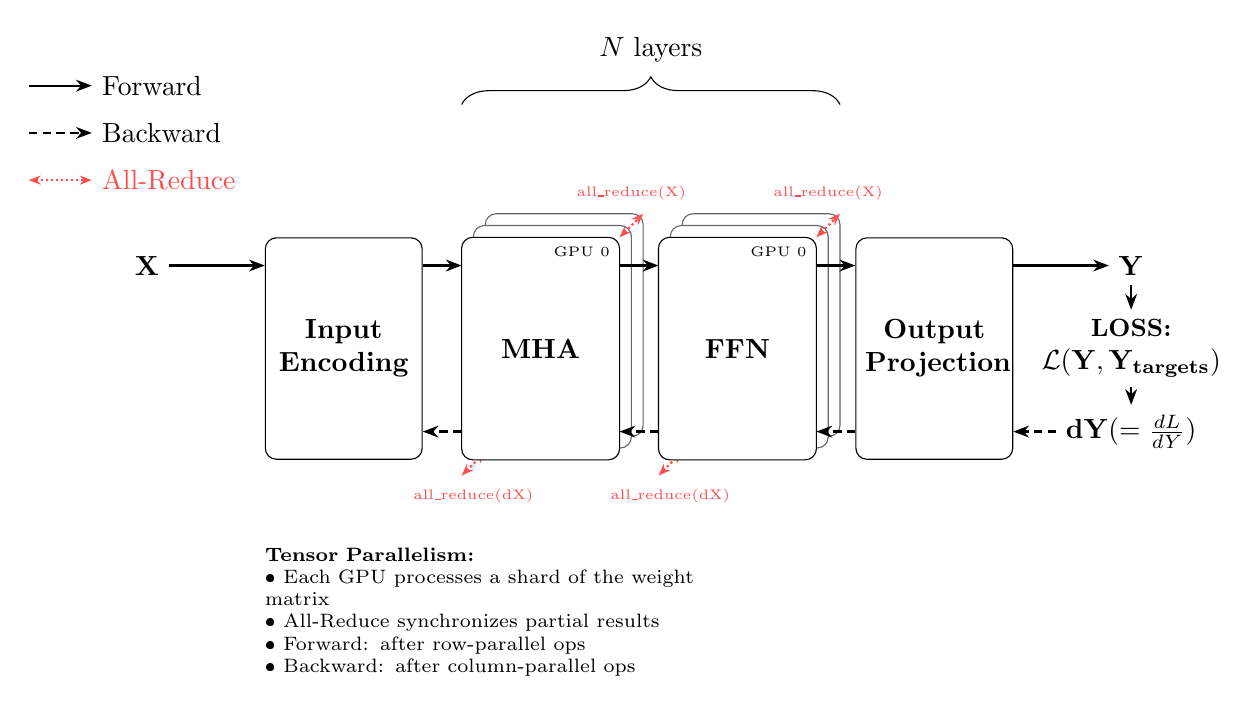
\begin{tikzpicture}[
    node distance=2.5cm,
    >=stealth,
    block/.style={rectangle, draw=black, fill=white, text width=5em, text centered, rounded corners, minimum height=8em, font=\bfseries},
    blockstack/.style={rectangle, draw=black!60, fill=white, text width=5em, text centered, rounded corners, minimum height=8em},
    forward/.style={-{Stealth[length=2mm]}, thick, black},
    backward/.style={-{Stealth[length=2mm]}, thick, black, densely dashed},
    allreduce/.style={{Stealth[length=1.5mm]}-{Stealth[length=1.5mm]}, thick, red!70, densely dotted},
    io/.style={text centered, font=\bfseries}
]
    % Title
    % \node[font=\Large\bfseries] at (10, 6) {Transformer Overall Flow (TP with 3 GPUs)};

    % Forward path nodes (horizontal)
    \node (input) [io] {$\mathbf{X}$};
    \node (encoding) [block, right of=input, yshift=-3em] {Input\\Encoding};

    % MHA blocks (3 stacked) - GPU 2 (back)
    \node (mha3) [blockstack, right of=encoding, xshift=0.3cm, yshift=0.3cm] {};
    % MHA blocks (3 stacked) - GPU 1 (middle)
    \node (mha2) [blockstack, right of=encoding, xshift=0.15cm, yshift=0.15cm] {};
    % MHA blocks (3 stacked) - GPU 0 (front)
    \node (mha) [block, right of=encoding] {MHA};

    % Small GPU labels for MHA
    \node[font=\tiny, anchor=north east] at (mha.north east) {GPU 0};

    % FFN blocks (3 stacked) - GPU 2 (back)
    \node (mlp3) [blockstack, right of=mha, xshift=0.3cm, yshift=0.3cm] {};
    % FFN blocks (3 stacked) - GPU 1 (middle)
    \node (mlp2) [blockstack, right of=mha, xshift=0.15cm, yshift=0.15cm] {};
    % FFN blocks (3 stacked) - GPU 0 (front)
    \node (mlp) [block, right of=mha] {FFN};

    % Small GPU labels for FFN
    \node[font=\tiny, anchor=north east] at (mlp.north east) {GPU 0};

    \node (output) [block, right of=mlp] {Output\\Projection};
    \node (pred) [io, right of=output, yshift=3em] {$\mathbf{Y}$};
    \node (loss) [align=center, io, right of=output] {\small LOSS:\\$\mathcal{L}(\mathbf{Y,Y_\text{targets}})$};
    \node (gradient) [io, right of=output, yshift=-3em] {$\mathbf{dY}(=\frac{dL}{dY})$};

    % All-Reduce arrows (Backward drawn first, then blocks, then Forward on top)
    % Backward All-Reduce - FFN (left-bottom corner, lower position)
    \draw [allreduce] ([yshift=-0.2cm]mlp.south west) -- ([xshift=0.3cm, yshift=0.1cm]mlp.south west);
    \node[font=\tiny, red!70, anchor=north] at ([xshift=0.15cm, yshift=-0.25cm]mlp.south west) {all\_reduce(dX)};

    % Backward All-Reduce - MHA (left-bottom corner, lower position)
    \draw [allreduce] ([yshift=-0.2cm]mha.south west) -- ([xshift=0.3cm, yshift=0.1cm]mha.south west);
    \node[font=\tiny, red!70, anchor=north] at ([xshift=0.15cm, yshift=-0.25cm]mha.south west) {all\_reduce(dX)};

    % Redraw blocks to cover backward All-Reduce arrows
    \draw [draw=black!60, fill=white, rounded corners] (mha3.south west) rectangle (mha3.north east);
    \draw [draw=black!60, fill=white, rounded corners] (mha2.south west) rectangle (mha2.north east);
    \draw [draw=black, fill=white, rounded corners, line width=0.4pt] (mha.south west) rectangle (mha.north east);
    \node[font=\bfseries] at (mha.center) {MHA};
    \node[font=\tiny, anchor=north east] at (mha.north east) {GPU 0};

    \draw [draw=black!60, fill=white, rounded corners] (mlp3.south west) rectangle (mlp3.north east);
    \draw [draw=black!60, fill=white, rounded corners] (mlp2.south west) rectangle (mlp2.north east);
    \draw [draw=black, fill=white, rounded corners, line width=0.4pt] (mlp.south west) rectangle (mlp.north east);
    \node[font=\bfseries] at (mlp.center) {FFN};
    \node[font=\tiny, anchor=north east] at (mlp.north east) {GPU 0};

    % Forward All-Reduce - MHA (right-top corner) - drawn after blocks to appear on top
    \draw [allreduce] (mha.north east) -- ([xshift=0.3cm, yshift=0.3cm]mha.north east);
    \node[font=\tiny, red!70, anchor=south] at ([xshift=0.15cm, yshift=0.35cm]mha.north east) {all\_reduce(X)};

    % Forward All-Reduce - FFN (right-top corner) - drawn after blocks to appear on top
    \draw [allreduce] (mlp.north east) -- ([xshift=0.3cm, yshift=0.3cm]mlp.north east);
    \node[font=\tiny, red!70, anchor=south] at ([xshift=0.15cm, yshift=0.35cm]mlp.north east) {all\_reduce(X)};

    % Forward arrows (upper part of blocks)
    \draw [forward] (input) -- ([yshift=3em]encoding.west);
    \draw [forward] ([yshift=3em]encoding.east) -- ([yshift=3em]mha.west);
    \draw [forward] ([yshift=3em]mha.east) -- ([yshift=3em]mlp.west);
    \draw [forward] ([yshift=3em]mlp.east) -- ([yshift=3em]output.west);
    \draw [forward] ([yshift=3em]output.east) -- (pred);
    \draw [forward] (pred) -- (loss);
    \draw [backward] (loss) -- (gradient);

    % Backward arrows (lower part of blocks)
    \draw [backward] (gradient) -- ([yshift=-3em]output.east);
    \draw [backward] ([yshift=-3em]output.west) -- ([yshift=-3em]mlp.east);
    \draw [backward] ([yshift=-3em]mlp.west) -- ([yshift=-3em]mha.east);
    \draw [backward] ([yshift=-3em]mha.west) -- ([yshift=-3em]encoding.east);

    % Brace for layer repetition (horizontal - using mlp with x offset to match mlp3)
    \draw[decorate, decoration={brace, amplitude=10pt}]
        ([yshift=4.8em]mha.north west) -- ([xshift=0.3cm, yshift=4.8em]mlp.north east)
        node[midway, above=12pt, font=\normalsize] {$N$ layers};

    % Labels (Legend)
    \coordinate (legend) at ([xshift=-1.5cm, yshift=6.5em]input);
    \draw[forward] (legend) -- ++(0.8,0) node[right, font=\normalsize] {Forward};
    \draw[backward] ([yshift=-0.6cm]legend) -- ++(0.8,0) node[right, font=\normalsize] {Backward};
    \draw[allreduce] ([yshift=-1.2cm]legend) -- ++(0.8,0) node[right, font=\normalsize] {All-Reduce};

    % TP explanation
    \node[font=\scriptsize, align=left, text width=6cm] at ([xshift=2cm, yshift=-5.5em]encoding.south) {
        \textbf{Tensor Parallelism:}\\
        • Each GPU processes a shard of the weight matrix\\
        • All-Reduce synchronizes partial results\\
        • Forward: after row-parallel ops\\
        • Backward: after column-parallel ops
    };

\end{tikzpicture}%
}

\clearpage

\subsection{MHA with Tensor Parallelism}

\subsubsection{Forward Pass}

\begin{landscape}
\thispagestyle{fancy}
\resizebox{\linewidth}{!}{%
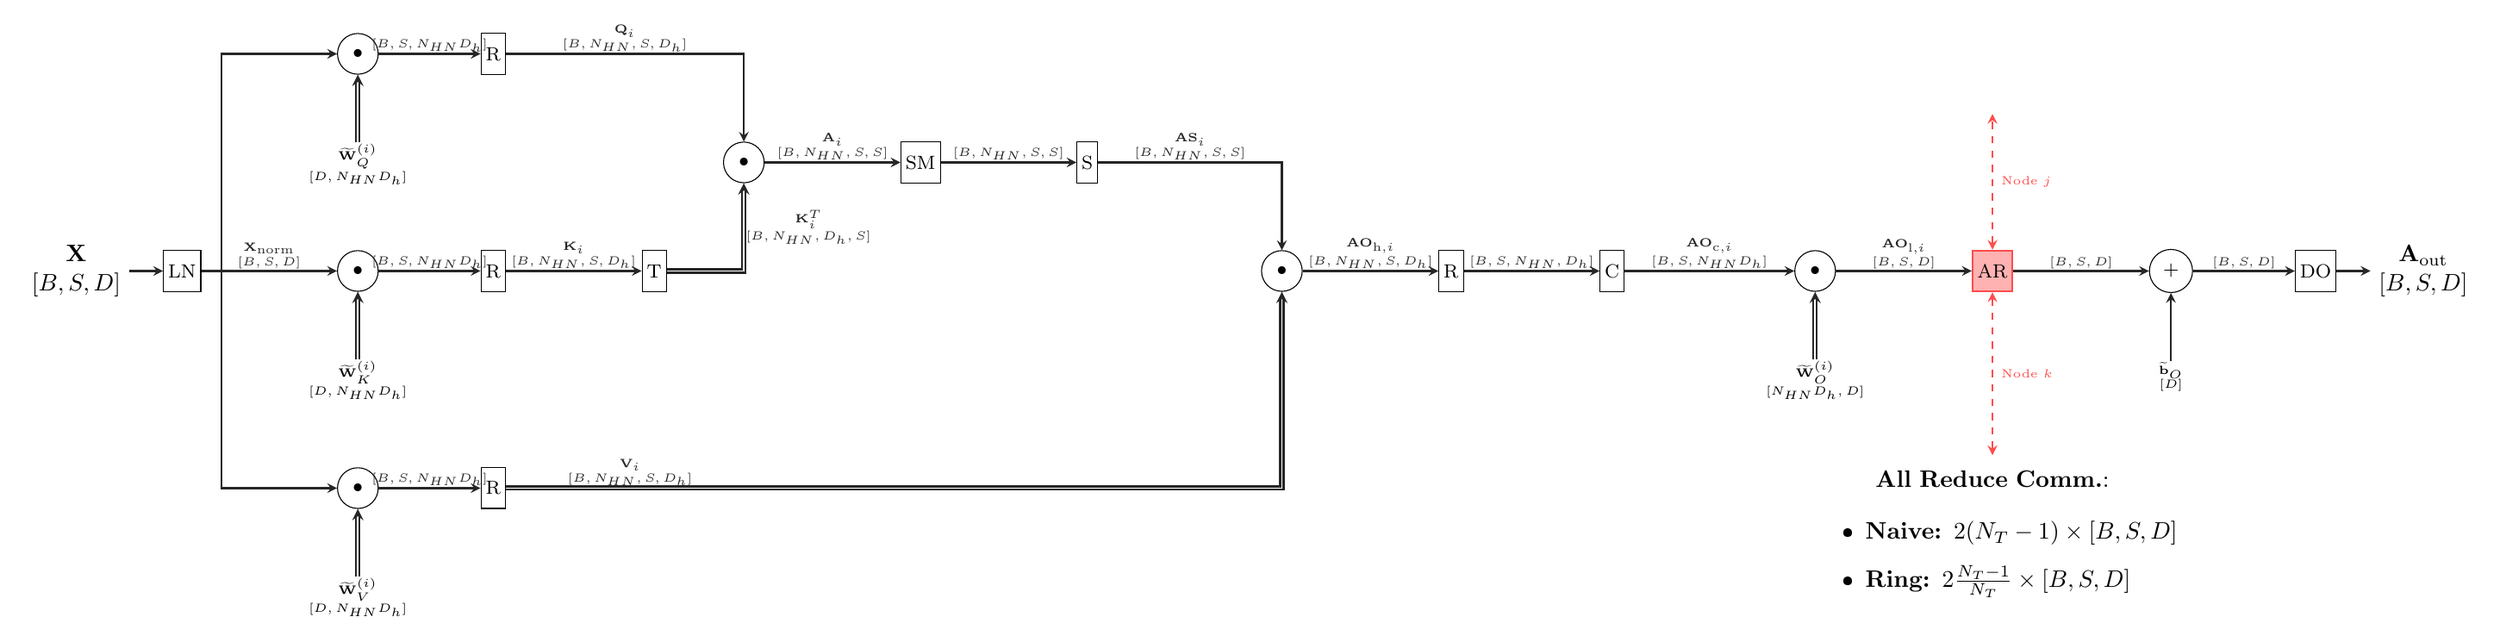
\begin{tikzpicture}[
  every node/.style={transform shape},
  >=stealth,
  auxnode/.style={draw, rectangle, fill=white, minimum height=6mm, inner sep=2pt, font=\footnotesize, align=center},
  mulnode/.style={draw, circle, fill=white, minimum size=6mm, font=\footnotesize, align=center},
  addnode/.style={draw, circle, fill=white, minimum size=6mm, font=\footnotesize, align=center},
  allreduce/.style={draw, rectangle, fill=red!30, minimum height=6mm, inner sep=2pt, font=\footnotesize, align=center, thick, draw=red!70},
  flow/.style={->, thick, black!85},
  flow2/.style={->, double, thick, black!85},
  commflow/.style={<->, thick, red!70, dashed},
  dimlabel/.style={font=\tiny, inner sep=0.5pt, align=center}
]
% \node[font=\Large\bfseries] at (9, 4.5) {Multi-Head Attention Forward Pass (Node $i$)};

\node (Input) at (0.5, 0) [align=center] {$\mathbf{X}$\\$[B,S,D]$};
\node[auxnode] (LN) [right=0.5cm of Input] {LN};

\node[mulnode] (Proj_Q) [right=2.0cm of LN, yshift=3.2cm] {$\bullet$};
\node[auxnode] (R_Q) [right=1.5cm of Proj_Q] {R};

\node[mulnode] (Proj_K) [right=2.0cm of LN, yshift=0cm] {$\bullet$};
\node[auxnode] (R_K) [right=1.5cm of Proj_K] {R};

\node[mulnode] (Proj_V) [right=2.0cm of LN, yshift=-3.2cm] {$\bullet$};
\node[auxnode] (R_V) [right=1.5cm of Proj_V] {R};

\node[dimlabel] (WQ) [align=center, below=1.0cm of Proj_Q] {$\widetilde{\mathbf{W}}_{Q}^{(i)}$\\$[D,N_{HN}D_h]$};
\node[dimlabel] (WK) [align=center, below=1.0cm of Proj_K] {$\widetilde{\mathbf{W}}_{K}^{(i)}$\\$[D,N_{HN}D_h]$};
\node[dimlabel] (WV) [align=center, below=1.0cm of Proj_V] {$\widetilde{\mathbf{W}}_{V}^{(i)}$\\$[D,N_{HN}D_h]$};

\node[auxnode] (T_K) [right=2.0cm of R_K] {T};
\node[mulnode] (QK) [right=3.2cm of R_Q, yshift=-1.6cm] {$\bullet$};
\node[auxnode] (SM) [right=2.0cm of QK] {SM};
\node[auxnode] (Soft) [right=2.0cm of SM] {S};
\node[mulnode] (PV) [right=2.4cm of Soft, yshift=-1.6cm] {$\bullet$};

\node[auxnode] (R_Merge) [right=2.0cm of PV] {R};
\node[auxnode] (Cat) [right=2.0cm of R_Merge] {C};

\node[mulnode] (OProj) [right=2.5cm of Cat] {$\bullet$};
\node[dimlabel] (WO_FWD) [align=center, below=1.0cm of OProj] {$\widetilde{\mathbf{W}}_{O}^{(i)}$\\$[N_{HN}D_h,D]$};
\node[allreduce] (AR) [right=2.0cm of OProj] {AR};
\node[
  align=center,
  below=2.5cm of AR,
  text width=5.5cm % 적당한 값으로 조정
] (AR_info) {%
  \textbf{All Reduce Comm.}:\\[2pt]
  \begin{itemize}
    \item \textbf{Naive:} $2(N_T-1) \times [B,S,D]$
    \item \textbf{Ring:} $2\frac{N_T-1}{N_T} \times [B,S,D]$
  \end{itemize}
};
\node[addnode] (AddB) [right=2.0cm of AR] {+};
\node[dimlabel] (BO) [align=center, below=1.0cm of AddB] {$\widetilde{\mathbf{b}}_{O}$\\$[D]$};
\node[auxnode] (Drop) [right=1.5cm of AddB] {DO};
\node (Aout) [align=center, right=0.5cm of Drop] {$\mathbf{A}_{\text{out}}$\\$[B,S,D]$};

\draw[flow] (Input) -- (LN);

\draw[flow] (LN.east) -- ++(0.3,0) |- (Proj_Q.west);
\draw[flow] (LN) -- (Proj_K.west) node[dimlabel, midway, above]{$\mathbf{X}_{\text{norm}}$\\$[B,S,D]$};
\draw[flow] (LN.east) -- ++(0.3,0) |- (Proj_V.west);

\draw[flow2] (WQ) -- (Proj_Q);
\draw[flow2] (WK) -- (Proj_K);
\draw[flow2] (WV) -- (Proj_V);

\draw[flow] (Proj_Q) -- (R_Q) node[dimlabel, midway, above]{$[B,S,N_{HN}D_h]$};
\draw[flow] (Proj_K) -- (R_K) node[dimlabel, midway, above]{$[B,S,N_{HN}D_h]$};
\draw[flow] (Proj_V) -- (R_V) node[dimlabel, midway, above]{$[B,S,N_{HN}D_h]$};

\draw[flow] (R_Q) -| (QK) node[dimlabel, near start, above]{$\mathbf{Q}_i$\\$[B,N_{HN},S,D_h]$};
\draw[flow] (R_K) -- (T_K) node[dimlabel, midway, above]{$\mathbf{K}_i$\\$[B,N_{HN},S,D_h]$};
\draw[flow2] (T_K) -| (QK) node[dimlabel, near end, right]{$\mathbf{K}_i^{T}$\\$[B,N_{HN},D_h,S]$};

\draw[flow] (QK) -- (SM) node[dimlabel, midway, above]{$\mathbf{A}_i$\\$[B,N_{HN},S,S]$};
\draw[flow] (SM) -- (Soft) node[dimlabel, midway, above]{$[B,N_{HN},S,S]$};
\draw[flow] (Soft) -| (PV) node[dimlabel, near start, above]{$\mathbf{AS}_i$\\$[B,N_{HN},S,S]$};
\draw[flow2] (R_V) -| (PV) node[dimlabel, pos=0.08, above]{$\mathbf{V}_i$\\$[B,N_{HN},S,D_h]$};

\draw[flow] (PV) -- (R_Merge) node[dimlabel, midway, above]{$\mathbf{AO}_{\text{h},i}$\\$[B,N_{HN},S,D_h]$};
\draw[flow] (R_Merge) -- (Cat) node[dimlabel, midway, above]{$[B,S,N_{HN},D_h]$};
\draw[flow] (Cat) -- (OProj) node[dimlabel, midway, above]{$\mathbf{AO}_{\text{c},i}$\\$[B,S,N_{HN}D_h]$};
\draw[flow2] (WO_FWD) -- (OProj);
\draw[flow] (OProj) -- (AR) node[dimlabel, midway, above]{$\mathbf{AO}_{\text{l},i}$\\$[B,S,D]$};

% All-Reduce communication arrows
\draw[commflow] (AR.north) -- ++(0, 2.0) node[midway, right, font=\tiny]{Node $j$};
\draw[commflow] (AR.south) -- ++(0, -2.4) node[midway, right, font=\tiny]{Node $k$};

\draw[flow] (AR) -- (AddB) node[dimlabel, midway, above]{$[B,S,D]$};
\draw[flow] (BO) -- (AddB);
\draw[flow] (AddB) -- (Drop) node[dimlabel, midway, above]{$[B,S,D]$};
\draw[flow] (Drop) -- (Aout);
\end{tikzpicture}%
}
\end{landscape}
\clearpage

\subsubsection{Backward Pass}

\begin{landscape}
\thispagestyle{fancy}
\par\vspace{1cm}
\noindent
\resizebox{\linewidth}{!}{%
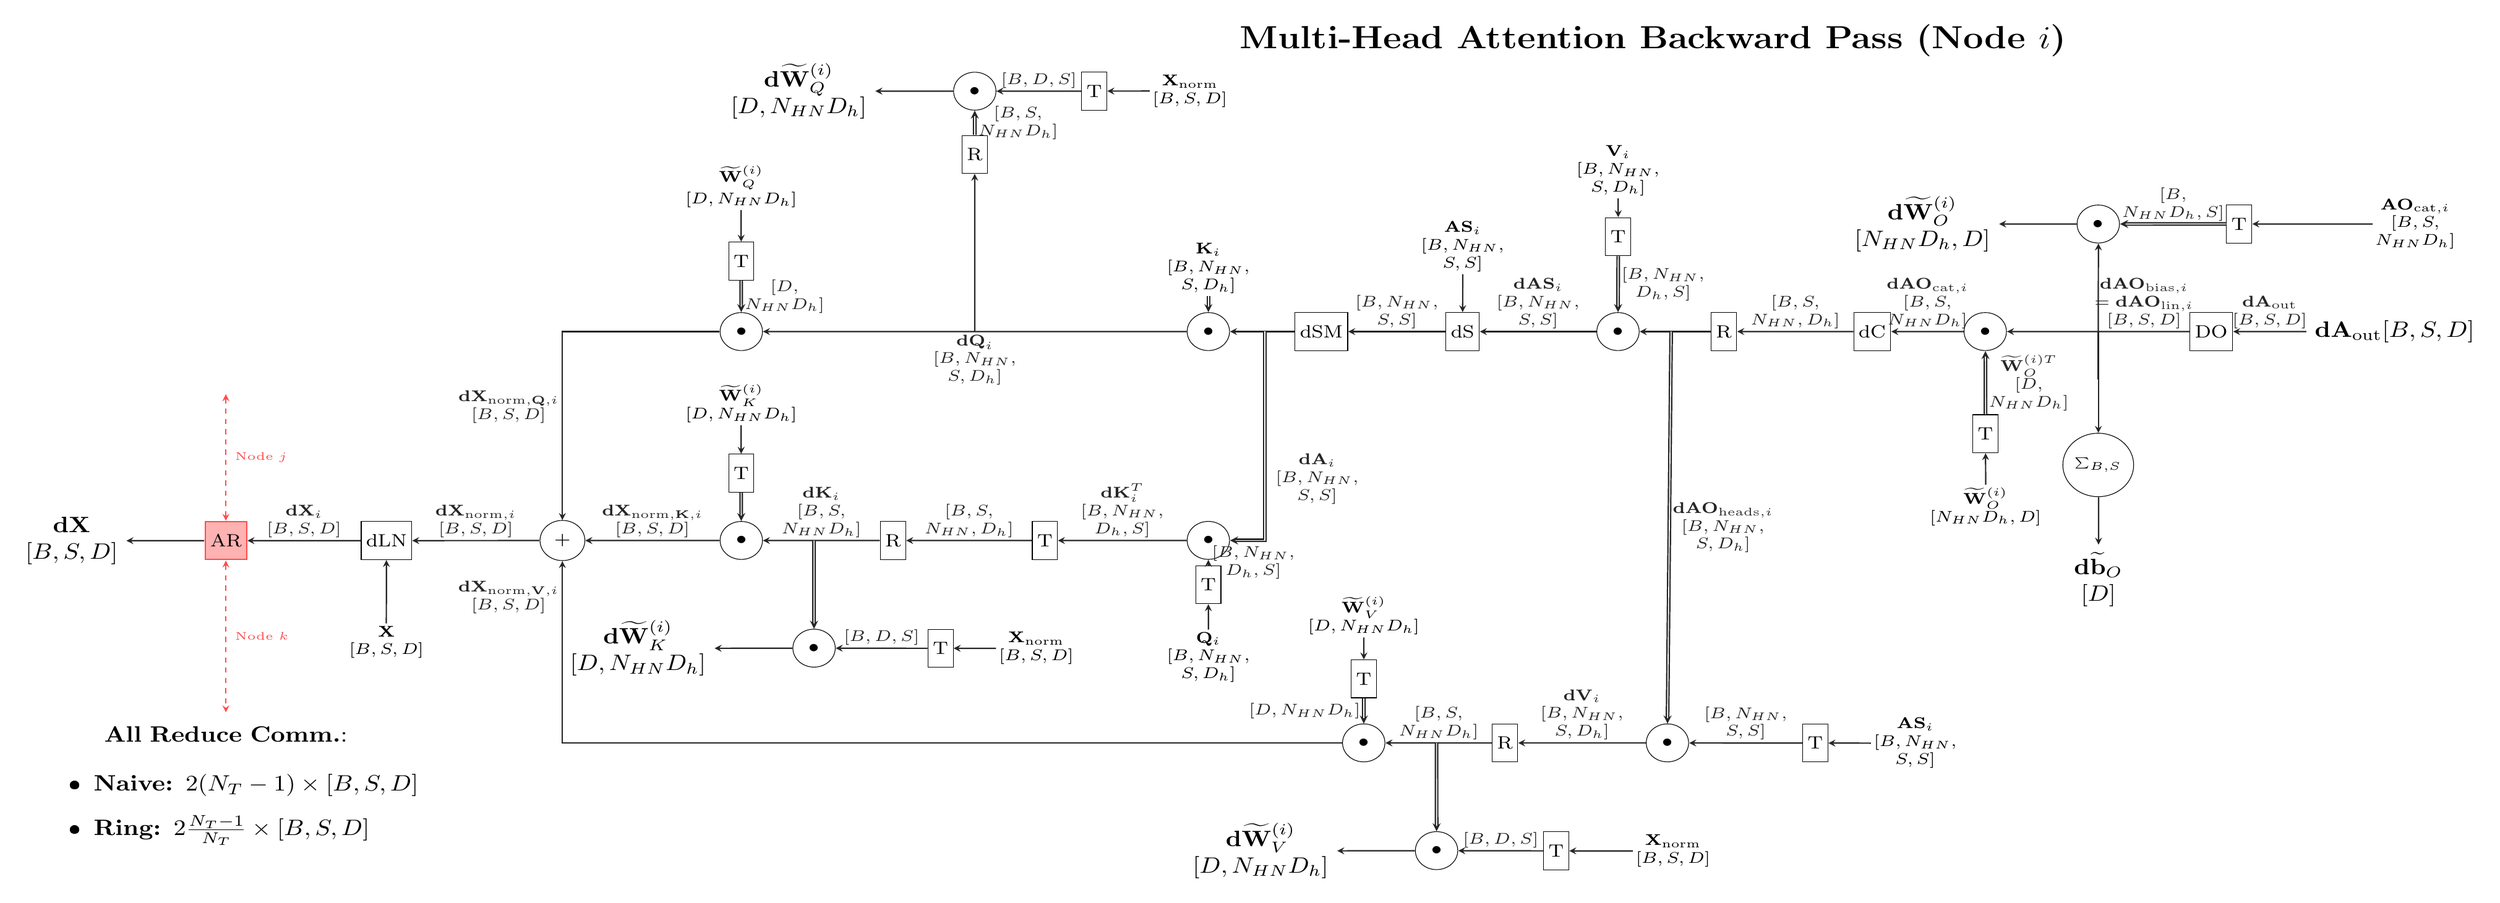
\begin{tikzpicture}[
  every node/.style={transform shape},
  >=stealth,
  auxnode/.style={draw, rectangle, fill=white, minimum height=6mm, inner sep=2pt, font=\footnotesize, align=center},
  mulnode/.style={draw, circle, fill=white, minimum size=6mm, font=\footnotesize, align=center},
  addnode/.style={draw, circle, fill=white, minimum size=6mm, font=\footnotesize, align=center},
  sumnode/.style={draw, circle, fill=white, minimum size=6mm, font=\tiny, align=center},
  allreduce/.style={draw, rectangle, fill=red!30, minimum height=6mm, inner sep=2pt, font=\footnotesize, align=center, thick, draw=red!70},
  flow/.style={->, thick, black!85},
  flow2/.style={->, double, thick, black!85},
  commflow/.style={<->, thick, red!70, dashed},
  dimlabel/.style={font=\scriptsize, inner sep=1pt, align=center},
  gradflow/.style={->, thick, black!85},
  gradweight/.style={->, thick, black!85}
]

\begin{scope}[xscale=1.45, yscale=1.3]

\def\yoffset{-1.0}
\def\dVXyoffset{-6.5}

\coordinate (Grad_Aout_B) at (17.5, \yoffset);
\coordinate (dDrop_center) at (15.9, \yoffset);
\coordinate (ProjGradSplit) at (14.3, \yoffset);
\coordinate (dOProj_center) at (12.7, \yoffset);
\coordinate (C_center) at (11.1, \yoffset);
\coordinate (R_center) at (9.0, \yoffset);
\coordinate (dPV_AS_calc_center) at (7.5, \yoffset);
\coordinate (dSoft_center) at (5.3, \yoffset);
\coordinate (dSM_calc_center) at (3.3, \yoffset);
\coordinate (dV_calc_center) at (8.2, \dVXyoffset+\yoffset);
\coordinate (R_V_bwd_center) at (5.9, \dVXyoffset+\yoffset);
\coordinate (dVX_calc_center) at (3.9, \dVXyoffset+\yoffset);
\coordinate (dQK_calc_Q_center) at (1.7, \yoffset);
\coordinate (dQK_calc_K_center) at (1.7, -3.3+\yoffset);
\coordinate (K_BWD_input_center) at (1.7, 1.0+\yoffset);
\coordinate (T_Q_bwd_center) at (1.7, -4.0+\yoffset);

\node[font=\Large\bfseries] at (8, 4.6+\yoffset) {Multi-Head Attention Backward Pass (Node $i$)};

\node (Grad_Aout_B) at (18.5, \yoffset) {$\mathbf{dA}_{\text{out}}$\\$[B,S,D]$};
\node[auxnode] (DO) at (dDrop_center) {DO};
\node[mulnode] (dOProj) at (dOProj_center) {$\bullet$};

\node[auxnode] (T_WO) [below=1.0cm of dOProj] {T};
\node[dimlabel] (WO_BWD) [below=0.5cm of T_WO] {$\widetilde{\mathbf{W}}_{O}^{(i)}$\\$[N_{HN}D_h,D]$};

\node[mulnode] (dWO_calc) at ($(ProjGradSplit)+(0, 1.7)$) {$\bullet$};
\node[align=center, left=1.1cm of dWO_calc]
  (dWO_GRAD) {$\mathbf{d}\widetilde{\mathbf{W}}_{O}^{(i)}$\\$[N_{HN}D_h,D]$};
\node[auxnode] (T_AO_in) [right=1.5cm of dWO_calc] {T};
\node[dimlabel] (AO_in_local_label) [right=1.7cm of T_AO_in] {$\mathbf{AO}_{\text{cat},i}$\\$[B,S,$\\$N_{HN}D_h]$};

\node[auxnode] (C) at (C_center) {dC};
\node[auxnode] (R) at (R_center) {R};

\node[mulnode] (dPV_AS_calc) at (dPV_AS_calc_center) {$\bullet$};
\node[auxnode] (dSoft) at (dSoft_center) {dS};
\node[auxnode] (dSM_calc) at (dSM_calc_center) {dSM};

\node[mulnode] (dQK_calc_Q) at (dQK_calc_Q_center) {$\bullet$};
\node[mulnode] (dQX_proj_calc) [left=6.0cm of dQK_calc_Q] {$\bullet$};

\node[mulnode] (dQK_calc_K) at (dQK_calc_K_center) {$\bullet$};
\node[mulnode] (dKX_proj_calc) [left=6.0cm of dQK_calc_K] {$\bullet$};

\node[dimlabel] (K_BWD_input) at (K_BWD_input_center) {$\mathbf{K}_i$\\$[B,N_{HN},$\\$S,D_h]$};
\node[auxnode] (T_Q_bwd) at (T_Q_bwd_center) {T};
\node[dimlabel] (Q_BWD_input) [below=0.4cm of T_Q_bwd] {$\mathbf{Q}_i$\\$[B,N_{HN},$\\$S,D_h]$};

\node[dimlabel] (V_FWD) [above=1.8cm of dPV_AS_calc] {$\mathbf{V}_i$\\$[B,N_{HN},$\\$S,D_h]$};
\node[auxnode] (T_V_bwd) [below=0.3cm of V_FWD] {T};

\node[mulnode] (dV_calc) at (dV_calc_center) {$\bullet$};
\node[auxnode] (T_AS_bwd) [right=1.6cm of dV_calc] {T};
\node[dimlabel] (AS_BWD_for_V) [right=0.6cm of T_AS_bwd] {$\mathbf{AS}_i$\\$[B,N_{HN},$\\$S,S]$};

\node[auxnode] (R_V_bwd) at (R_V_bwd_center) {R};
\node[mulnode] (dVX_calc) at (dVX_calc_center) {$\bullet$};

\node[auxnode] (T_WV) [above=0.4cm of dVX_calc] {T};
\node[dimlabel] (WV_BWD) [above=0.35cm of T_WV] {$\widetilde{\mathbf{W}}_{V}^{(i)}$\\$[D,N_{HN}D_h]$};

\node[sumnode] (Sum_dBO) [below=1.6cm of ProjGradSplit] {$\sum_{B, S}$};
\node (dBO) [align=center, below=0.75cm of Sum_dBO] {$\mathbf{d}\widetilde{\mathbf{b}}_{O}$\\$[D]$};

\draw[gradflow] (Grad_Aout_B) -- (DO)
  node[dimlabel, midway, above]{$\mathbf{dA}_{\text{out}}$\\$[B,S,D]$};

\draw[gradflow] (DO) -- (dOProj)
  node[dimlabel, pos=0.25, above]{$\mathbf{dAO}_{\text{bias},i}$\\$=\mathbf{dAO}_{\text{lin},i}$\\$[B,S,D]$};

\draw[gradflow] (ProjGradSplit) -- (dWO_calc.south);
\draw[gradflow] (ProjGradSplit) -- ([yshift=-0.75cm]ProjGradSplit) -| (Sum_dBO.north);

\draw[gradflow] (dOProj) -- (C)
  node[dimlabel, midway, above]{$\mathbf{dAO}_{\text{cat},i}$\\$[B,S,$\\$N_{HN}D_h]$};
\draw[gradflow] (C) -- (R)
  node[dimlabel, midway, above]{$[B,S,$\\$N_{HN},D_h]$};

\coordinate (R_split_point) at ($(dPV_AS_calc)!0.5!(R)$);
\draw[gradflow] (R.west) -- (dPV_AS_calc.east);
\draw[flow2] (R_split_point) -- (dV_calc.north)
  node[dimlabel, midway, right]{$\mathbf{dAO}_{\text{heads},i}$\\$[B,N_{HN},$\\$S,D_h]$};

\draw[gradflow] (V_FWD.south) -- (T_V_bwd.north);
\draw[flow2] (T_V_bwd.south) -- (dPV_AS_calc.north)
  node[dimlabel, midway, right]{$[B,N_{HN},$\\$D_h,S]$};
\draw[gradflow] (dPV_AS_calc.west) -- (dSoft.east)
  node[dimlabel, midway, above]{$\mathbf{dAS}_i$\\$[B,N_{HN},$\\$S,S]$};

\node (AS_BWD_dS) [dimlabel, above=0.6cm of dSoft] {$\mathbf{AS}_i$\\$[B,N_{HN},$\\$S,S]$};
\draw[gradflow] (AS_BWD_dS.south) -- (dSoft.north);
\draw[gradflow] (dSoft.west) -- (dSM_calc.east)
  node[dimlabel, midway, above]{$[B,N_{HN},$\\$S,S]$};

\coordinate (dA_Split_X) at ($(dSM_calc_center)!0.5!(dQK_calc_Q_center)$);
\coordinate (dA_Split) at (dA_Split_X |- dQK_calc_Q.east);
\draw[gradflow] (dSM_calc.west) -- (dQK_calc_Q.east);
\draw[flow2] (dA_Split) -- (dA_Split |- dQK_calc_K.east) -- (dQK_calc_K.east)
  node[dimlabel, pos=-1.5, above, yshift=15]{$\mathbf{dA}_i$\\$[B,N_{HN},$\\$S,S]$};

\draw[flow2] (K_BWD_input.south) -- (dQK_calc_Q.north);
\draw[gradweight] (dQK_calc_Q) -- (dQX_proj_calc)
  node[dimlabel, midway, below]{$\mathbf{dQ}_i$\\$[B,N_{HN},$\\$S,D_h]$};

\node[auxnode] (T_WQ_bwd) [above=0.5cm of dQX_proj_calc] {T};
\node[dimlabel] (WQ_bwd) [above=0.5cm of T_WQ_bwd] {$\widetilde{\mathbf{W}}_{Q}^{(i)}$\\$[D,N_{HN}D_h]$};
\draw[flow] (WQ_bwd) -- (T_WQ_bwd);
\draw[flow2] (T_WQ_bwd.south) -- (dQX_proj_calc.north)
  node[dimlabel, midway, right]{$[D,$\\$N_{HN}D_h]$};

\draw[flow] (Q_BWD_input.north) -- (T_Q_bwd.south);
\draw[flow] (T_Q_bwd.north) -- (dQK_calc_K.south)
  node[dimlabel, pos=0.55, right]{$[B,N_{HN},$\\$D_h,S]$};

\node[auxnode] (T_dK) at ($(dQK_calc_K)!0.35!(dKX_proj_calc)$) {T};
\node[auxnode] (R_dK_mid) at ($(T_dK)!0.5!(dKX_proj_calc)$) {R};

\draw[gradweight] (dQK_calc_K) -- (T_dK)
  node[dimlabel, midway, above]{$\mathbf{dK}_i^T$\\$[B,N_{HN},$\\$D_h,S]$};
\draw[gradweight] (T_dK) -- (R_dK_mid)
  node[dimlabel, midway, above]{$[B,S,$\\$N_{HN},D_h]$};
\draw[gradweight] (R_dK_mid) -- (dKX_proj_calc)
  node[dimlabel, midway, above]{$\mathbf{dK}_i$\\$[B,S,$\\$N_{HN}D_h]$};

\node[auxnode] (T_WK_bwd) [above=0.45cm of dKX_proj_calc] {T};
\node[dimlabel] (WK_bwd) [above=0.45cm of T_WK_bwd] {$\widetilde{\mathbf{W}}_{K}^{(i)}$\\$[D,N_{HN}D_h]$};
\draw[gradflow] (WK_bwd) -- (T_WK_bwd);
\draw[flow2] (T_WK_bwd.south) -- (dKX_proj_calc.north);

\draw[gradflow] (AS_BWD_for_V.west) -- (T_AS_bwd.east);
\draw[gradflow] (T_AS_bwd.west) -- (dV_calc.east)
  node[dimlabel, midway, above]{$[B,N_{HN},$\\$S,S]$};
\draw[gradflow] (dV_calc.west) -- (R_V_bwd.east)
  node[dimlabel, midway, above]{$\mathbf{dV}_i$\\$[B,N_{HN},$\\$S,D_h]$};
\draw[gradflow] (R_V_bwd) -- (dVX_calc.east)
  node[dimlabel, midway, above]{$[B,S,$\\$N_{HN}D_h]$};

\draw[gradflow] (WV_BWD) -- (T_WV);
\draw[flow2] (T_WV) -- (dVX_calc.north)
  node[dimlabel, midway, left]{$[D,N_{HN}D_h]$};

\node[addnode] (Sum_dXnorm) [left=1.9cm of dKX_proj_calc] {$+$};

\draw[gradweight] (dQX_proj_calc.west) -| node[dimlabel, pos=0.7, left]{$\mathbf{dX}_{\text{norm},\mathbf{Q},i}$\\$[B,S,D]$} (Sum_dXnorm.north);
\draw[gradweight] (dKX_proj_calc.west) -- node[dimlabel, midway, above]{$\mathbf{dX}_{\text{norm},\mathbf{K},i}$\\$[B,S,D]$} (Sum_dXnorm.east);
\draw[gradweight] (dVX_calc.west) -| node[dimlabel, pos=0.9, left]{$\mathbf{dX}_{\text{norm},\mathbf{V},i}$\\$[B,S,D]$} (Sum_dXnorm.south);

\coordinate (dV_branch) at ($(R_V_bwd.west)!0.52!(dVX_calc.east)$);
\node[mulnode] (dWV_mul) at ($(dV_branch)+(0,-1.7cm)$) {$\bullet$};
\draw[flow2] (dV_branch) -- (dWV_mul.north);

\node[auxnode] (T_Xnorm) [right=1.2cm of dWV_mul] {T};
\node[dimlabel] (Xnorm_local) [right=0.9cm of T_Xnorm] {$\mathbf{X}_{\text{norm}}$\\$[B,S,D]$};
\draw[gradflow] (Xnorm_local) -- (T_Xnorm);
\draw[gradflow] (T_Xnorm.west) -- (dWV_mul.east)
  node[dimlabel, midway, above]{$[B,D,S]$};
\node (dWV_out) [align=center, left=1.1cm of dWV_mul] {$\mathbf{d}\widetilde{\mathbf{W}}_{V}^{(i)}$\\$[D,N_{HN}D_h]$};
\draw[gradweight] (dWV_mul.west) -- (dWV_out);

\coordinate (dQ_branch) at ($(dQK_calc_Q.east)!0.50!(dQX_proj_calc.west)$);
\node[mulnode] (dWQ_mul) at ($(dQ_branch)+(0,3.8cm)$) {$\bullet$};
\node[auxnode] (R_dQ_for_WQ) at ($(dWQ_mul)+(0,-1.0cm)$) {R};
\draw[gradflow]  (dQ_branch) -- (R_dQ_for_WQ.south);
\draw[flow2] (R_dQ_for_WQ.north) -- (dWQ_mul.south)
  node[dimlabel, midway, right]{$[B,S,$\\$N_{HN}D_h]$};

\node[auxnode] (T_XnormQ) [right=1.2cm of dWQ_mul] {T};
\node[dimlabel] (Xnorm_localQ) [right=0.6cm of T_XnormQ] {$\mathbf{X}_{\text{norm}}$\\$[B,S,D]$};
\draw[gradflow] (Xnorm_localQ) -- (T_XnormQ);
\draw[gradflow] (T_XnormQ.west) -- (dWQ_mul.east)
  node[dimlabel, midway, above]{$[B,D,S]$};
\node (dWQ_out) [align=center, left=1.1cm of dWQ_mul] {$\mathbf{d}\widetilde{\mathbf{W}}_{Q}^{(i)}$\\$[D,N_{HN}D_h]$};
\draw[gradweight] (dWQ_mul.west) -- (dWQ_out);

\coordinate (dK_branch) at ($(R_dK_mid)!0.52!(dKX_proj_calc)$);
\node[mulnode] (dWK_mul) at ($(dK_branch)+(0,-1.7cm)$) {$\bullet$};
\draw[flow2]  (dK_branch) -- (dWK_mul.north);

\node[auxnode] (T_XnormK) [right=1.3cm of dWK_mul] {T};
\node[dimlabel, right=0.6cm of T_XnormK] (Xnorm_localK) {$\mathbf{X}_{\text{norm}}$\\$[B,S,D]$};
\draw[gradflow] (Xnorm_localK) -- (T_XnormK);
\draw[gradflow] (T_XnormK.west) -- (dWK_mul.east)
  node[dimlabel, midway, above]{$[B,D,S]$};
\node (dWK_out) [align=center, left=1.1cm of dWK_mul] {$\mathbf{d}\widetilde{\mathbf{W}}_{K}^{(i)}$\\$[D,N_{HN}D_h]$};
\draw[gradweight] (dWK_mul.west) -- (dWK_out);

\draw[gradweight] (Sum_dBO) -- (dBO);

\draw[gradflow] (WO_BWD) -- (T_WO);
\draw[flow2] (T_WO) -- (dOProj)
  node[dimlabel, midway, right]{$\widetilde{\mathbf{W}}_{O}^{(i)T}$\\$[D,$\\$N_{HN}D_h]$};
\draw[gradflow] (AO_in_local_label) -- (T_AO_in);
\draw[flow2] (T_AO_in) -- (dWO_calc.east)
  node[dimlabel, midway, above]{$[B,$\\$N_{HN}D_h,S]$};
\draw[gradweight] (dWO_calc) -- (dWO_GRAD);

\node[auxnode] (dLN) [left=1.8cm of Sum_dXnorm] {dLN};
\draw[gradweight] (Sum_dXnorm.west) -- node[dimlabel, midway, above]
  {$\mathbf{dX}_{\text{norm},i}$\\$[B,S,D]$} (dLN.east);

\node[allreduce] (AR) [left=1.6cm of dLN] {AR};
\node[
  align=center,
  below=2.5cm of AR,
  text width=5.5cm
] (AR_info) {%
  \textbf{All Reduce Comm.}:\\[2pt]
  \begin{itemize}
    \item \textbf{Naive:} $2(N_T-1) \times [B,S,D]$
    \item \textbf{Ring:} $2\frac{N_T-1}{N_T} \times [B,S,D]$
  \end{itemize}
};

% All-Reduce communication arrows
\draw[commflow] (AR.north) -- ++(0, 2.0) node[midway, right, font=\tiny]{Node $j$};
\draw[commflow] (AR.south) -- ++(0, -2.4) node[midway, right, font=\tiny]{Node $k$};

\draw[gradweight] (dLN.west) -- (AR.east) node[dimlabel, midway, above]{$\mathbf{dX}_i$\\$[B,S,D]$};

\node (dX_OUT) [align=center, left=1.1cm of AR] {$\mathbf{dX}$\\$[B,S,D]$};
\draw[gradweight] (AR.west) -- (dX_OUT);

\node[dimlabel] (LNCache) [below=1.0cm of dLN] {$\mathbf{X}$\\$[B,S,D]$};
\draw[gradflow] (LNCache.north) -- (dLN.south);

\end{scope}
\end{tikzpicture}
}
\end{landscape}
\clearpage

\subsection{MLP with Tensor Parallelism}

\subsubsection{Forward Pass}
\resizebox{\linewidth}{!}{%
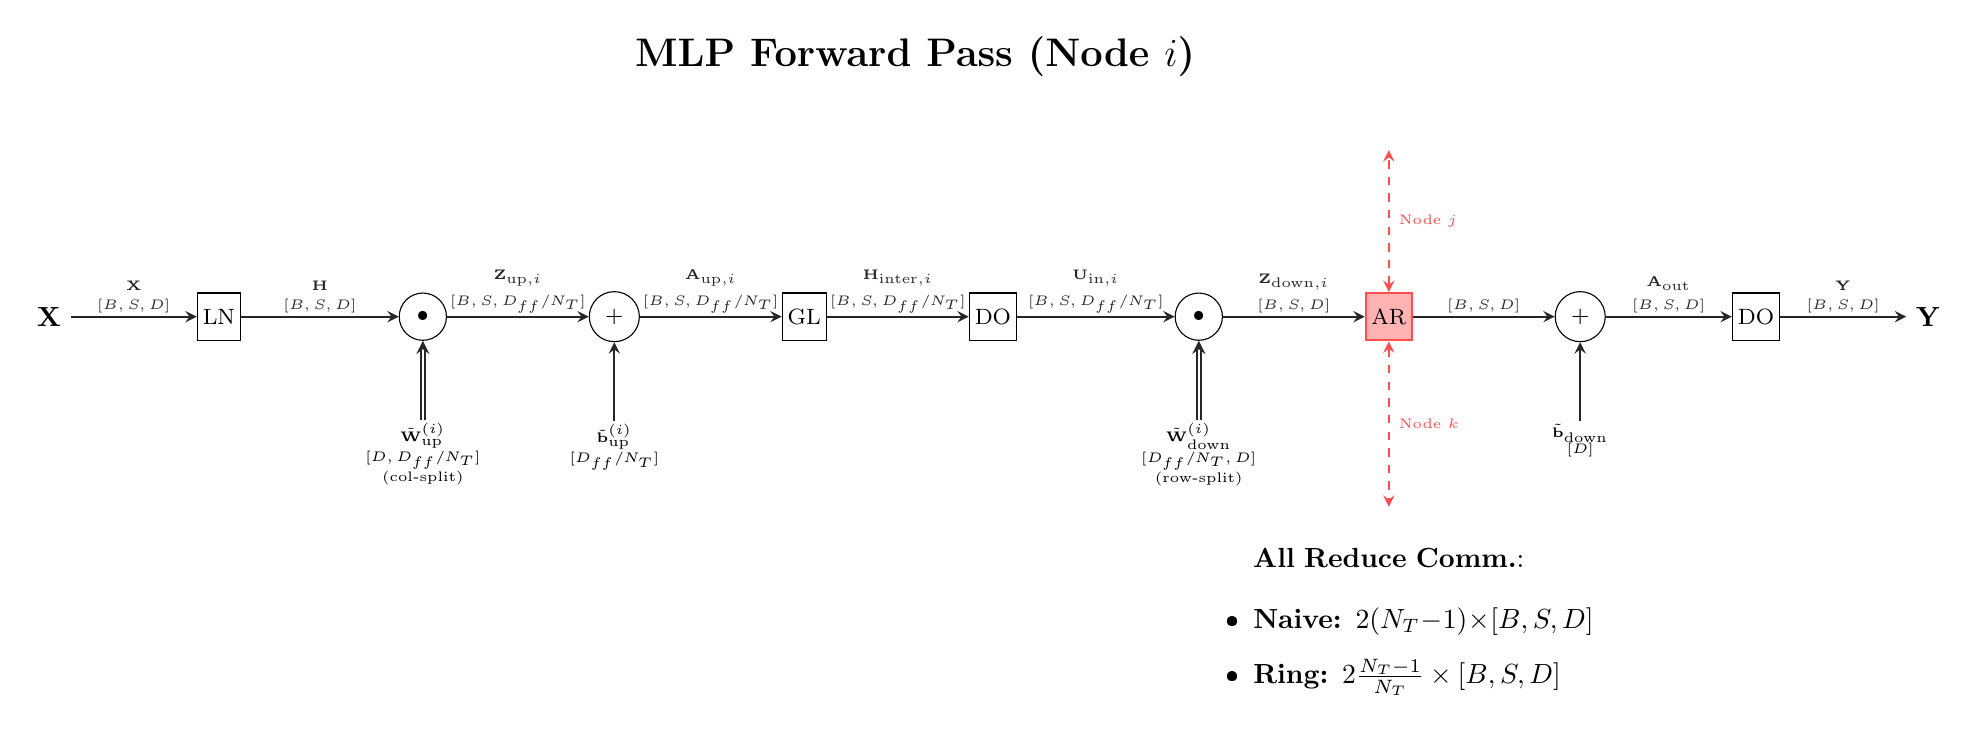
\begin{tikzpicture}[
    >=stealth,
    auxnode/.style={draw, rectangle, fill=white, minimum height=6mm, inner sep=2pt, font=\footnotesize, align=center},
    mulnode/.style={draw, circle, fill=white, minimum size=6mm, font=\footnotesize, align=center},
    addnode/.style={draw, circle, fill=white, minimum size=6mm, font=\footnotesize, align=center},
    allreduce/.style={draw, rectangle, fill=red!30, minimum height=6mm, inner sep=2pt, font=\footnotesize, align=center, thick, draw=red!70},
    sumnode/.style={draw, circle, fill=white, minimum size=6mm, font=\tiny, align=center},
    flow/.style={->, thick, black!85},
    flow2/.style={double, ->, thick, black!85},
    commflow/.style={<->, thick, red!70, dashed},
    dimlabel/.style={font=\tiny, inner sep=1pt, align=center}
]
    \node[font=\Large\bfseries] at (11, 2.8) {MLP Forward Pass (Node $i$)};

    \pgfmathsetmacro{\verticaloffset}{-0.5}

    \node            (MIn)   at (0,\verticaloffset) {$\mathbf{X}$};
    \node[auxnode]   (LN2)   [right=1.6cm of MIn] {LN};
    \node[mulnode]   (L1Mul) [right=2.0cm of LN2] {$\bullet$};
    \node[dimlabel]  (Wup)   [below=1.0cm of L1Mul] {$\tilde{\mathbf{W}}_{\text{up}}^{(i)}$\\$[D, D_{ff}/N_T]$\\(col-split)};
    \node[addnode]   (AddB1) [right=1.8cm of L1Mul] {+};
    \node[dimlabel]  (Bup)   [below=1.0cm of AddB1] {$\tilde{\mathbf{b}}_{\text{up}}^{(i)}$\\$[D_{ff}/N_T]$};
    \node[auxnode]   (Act)   [right=1.8cm of AddB1] {GL};
    \node[auxnode]   (Drop1) [right=1.8cm of Act] {DO};
    \node[mulnode]   (L2Mul) [right=2.0cm of Drop1] {$\bullet$};
    \node[dimlabel]  (Wdown) [below=1.0cm of L2Mul] {$\tilde{\mathbf{W}}_{\text{down}}^{(i)}$\\$[D_{ff}/N_T, D]$\\(row-split)};
    \node[allreduce] (AR)    [right=1.8cm of L2Mul] {AR};
    \node[
      align=center,
      below=2.5cm of AR,
      text width=5.2cm
    ] (AR_info) {%
      \textbf{All Reduce Comm.}:\\[2pt]
      \begin{itemize}
        \item \textbf{Naive:} $2(N_T-1) \times [B,S,D]$
        \item \textbf{Ring:} $2\frac{N_T-1}{N_T} \times [B,S,D]$
      \end{itemize}
    };
    \node[addnode]   (AddB2) [right=1.8cm of AR] {+};
    \node[dimlabel]  (Bdown) [below=1.0cm of AddB2] {$\tilde{\mathbf{b}}_{\text{down}}$\\$[D]$};
    \node[auxnode]   (Drop2) [right=1.6cm of AddB2] {DO};
    \node            (MOut)  [right=1.6cm of Drop2] {$\mathbf{Y}$};

    % All-Reduce communication arrows
    \draw[commflow] (AR.north) -- ++(0, 1.8) node[midway, right, font=\tiny]{Node $j$};
    \draw[commflow] (AR.south) -- ++(0, -2.1) node[midway, right, font=\tiny]{Node $k$};

    \draw[flow] (MIn) -- (LN2) node[dimlabel, midway, above]{\shortstack{$\mathbf{X}$\\$[B,S,D]$}};
    \draw[flow] (LN2) -- (L1Mul) node[dimlabel, midway, above]{\shortstack{$\mathbf{H}$\\$[B,S,D]$}};
    \draw[flow2] (Wup) -- (L1Mul);
    \draw[flow] (L1Mul) -- (AddB1) node[dimlabel, midway, above]{\shortstack{$\mathbf{Z}_{\text{up},i}$\\$[B,S,D_{ff}/N_T]$}};
    \draw[flow] (Bup) -- (AddB1);
    \draw[flow] (AddB1) -- (Act) node[dimlabel, midway, above]{\shortstack{$\mathbf{A}_{\text{up},i}$\\$[B,S,D_{ff}/N_T]$}};
    \draw[flow] (Act) -- (Drop1) node[dimlabel, midway, above]{\shortstack{$\mathbf{H}_{\text{inter},i}$\\$[B,S,D_{ff}/N_T]$}};
    \draw[flow] (Drop1) -- (L2Mul) node[dimlabel, midway, above]{\shortstack{$\mathbf{U}_{\text{in},i}$\\$[B,S,D_{ff}/N_T]$}};
    \draw[flow2] (Wdown) -- (L2Mul);
    \draw[flow] (L2Mul) -- (AR) node[dimlabel, midway, above]{\shortstack{$\mathbf{Z}_{\text{down},i}$\\$[B,S,D]$}};
    \draw[flow] (AR) -- (AddB2) node[dimlabel, midway, above]{\shortstack{$[B,S,D]$}};
    \draw[flow] (Bdown) -- (AddB2);
    \draw[flow] (AddB2) -- (Drop2) node[dimlabel, midway, above]{\shortstack{$\mathbf{A}_{\text{out}}$\\$[B,S,D]$}};
    \draw[flow] (Drop2) -- (MOut) node[dimlabel, midway, above]{\shortstack{$\mathbf{Y}$\\$[B,S,D]$}};

\end{tikzpicture}%
}

\clearpage

\subsubsection{Backward Pass}
\resizebox{\linewidth}{!}{%
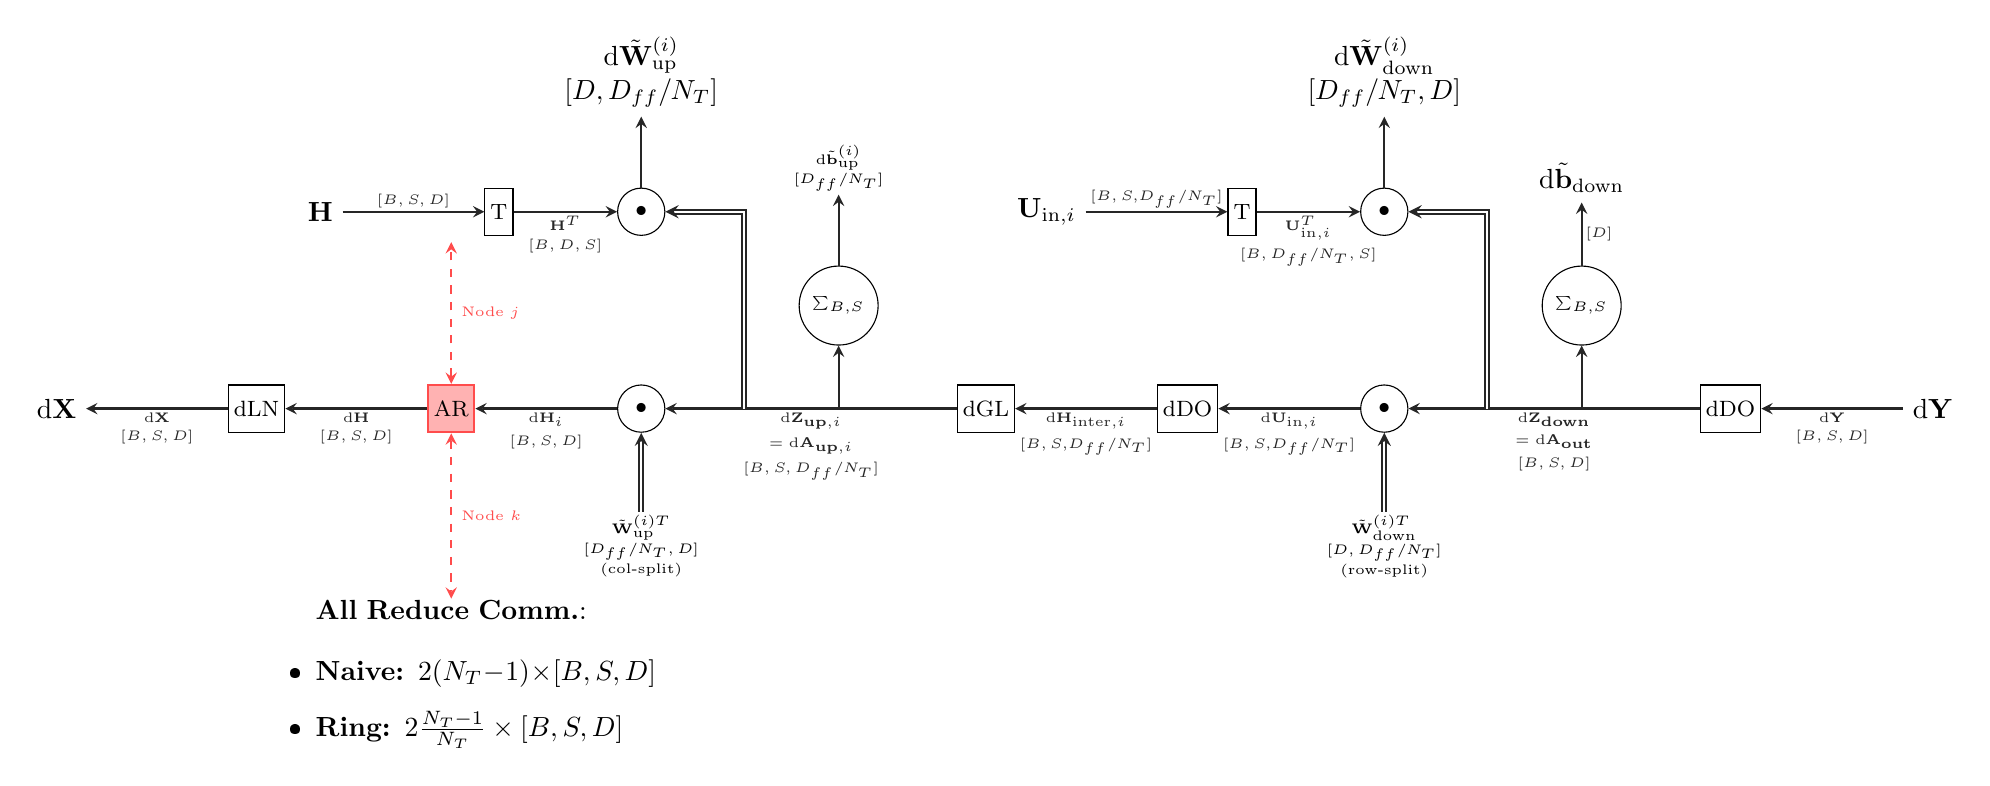
\begin{tikzpicture}[
    >=stealth,
    auxnode/.style={draw, rectangle, fill=white, minimum height=6mm, inner sep=2pt, font=\footnotesize, align=center},
    mulnode/.style={draw, circle, fill=white, minimum size=6mm, font=\footnotesize, align=center},
    addnode/.style={draw, circle, fill=white, minimum size=6mm, font=\footnotesize, align=center},
    sumnode/.style={draw, circle, fill=white, minimum size=6mm, font=\tiny, align=center},
    allreduce/.style={draw, rectangle, fill=red!30, minimum height=6mm, inner sep=2pt, font=\footnotesize, align=center, thick, draw=red!70},
    flow_rev/.style={<-, thick, black!85},
    flow_dw/.style={->, thick, black!85},
    flow_act/.style={double, ->, thick, black!85},
    commflow/.style={<->, thick, red!70, dashed},
    dimlabel/.style={font=\tiny, inner sep=1pt, align=center},
    gradlabel/.style={font=\tiny\bfseries, inner sep=1pt, align=center}
]
    % \node[font=\Large\bfseries] at (5, 10) {MLP Backward Pass (Node $i$)};

    \pgfmathsetmacro{\backwardoffset}{0.0}

    \node (d_MOut) at (12.6, \backwardoffset) {$\mathrm{d}\mathbf{Y}$};
    \node[auxnode] (d_Drop2) [left=1.8cm of d_MOut] {dDO};
    \draw[flow_rev] (d_Drop2) -- (d_MOut)
      node[dimlabel, midway, below]{\shortstack{$\mathrm{d}\mathbf{Y}$\\$[B,S,D]$}};

    \coordinate (split2) at ($(d_Drop2.west) + (-1.5cm, 0)$);
    \coordinate (branch_dUproj) at ($(split2) + (-1.2cm, 0)$);

    \node[sumnode] (d_SumB2) [above=0.8cm of split2] {$\sum_{B, S}$};
    \node (d_Bdown) [above=0.8cm of d_SumB2] {$\mathrm{d}\tilde{\mathbf{b}}_{\text{down}}$};
    \draw[flow_dw] (d_SumB2) -- (d_Bdown) node[dimlabel, midway, right]{$[D]$};

    \draw[flow_rev] (d_SumB2) -- (split2);

    \node[mulnode] (d_L2Mul_in) [left=2.2cm of split2] {$\bullet$};
    \draw[flow_rev] (d_L2Mul_in) -- (d_Drop2)
      node[gradlabel, midway, below]{\shortstack{$\mathrm{d}\mathbf{Z}_{\text{down}}$\\$=\mathrm{d}\mathbf{A}_{\text{out}}$\\$[B,S,D]$}};

    \node[dimlabel] (W_down_T) [align=center, below=1.0cm of d_L2Mul_in] {$\tilde{\mathbf{W}}_{\text{down}}^{(i)T}$\\$[D, D_{ff}/N_T]$\\(row-split)};
    \draw[flow_act] (W_down_T.north) -- (d_L2Mul_in);

    \coordinate (L2Mul_w_y) at ($(d_L2Mul_in) + (0, 2.5cm)$);
    \node[mulnode] (d_L2Mul_w) at (L2Mul_w_y) {$\bullet$};
    \node (d_Wdown) [align=center, above=0.9cm of d_L2Mul_w] {$\mathrm{d}\tilde{\mathbf{W}}_{\text{down}}^{(i)}$\\$[D_{ff}/N_T, D]$};
    \draw[flow_dw] (d_L2Mul_w) -- (d_Wdown);

    \draw[flow_act] (branch_dUproj.north) |- (d_L2Mul_w.east);

    \node[auxnode] (Uin_T) at ($(d_L2Mul_w.west) + (-1.5cm, 0)$) {T};
    \draw[flow_dw] (Uin_T) -- (d_L2Mul_w)
      node[dimlabel, midway, below]{\shortstack{$\mathbf{U}_{\text{in},i}^T$\\$[B, D_{ff}/N_T, S]$}};
    \node (Uin_aux) [left=1.8cm of Uin_T] {$\mathbf{U}_{\text{in},i}$};
    \draw[flow_dw] (Uin_aux) -- (Uin_T) node[dimlabel, midway, above]{\shortstack{$[B,S,$$D_{ff}/N_T]$}};

    \node[auxnode] (d_Drop1) [left=1.8cm of d_L2Mul_in] {dDO};
    \draw[flow_rev] (d_Drop1) -- (d_L2Mul_in)
      node[dimlabel, midway, below]{\shortstack{$\mathrm{d}\mathbf{U}_{\text{in},i}$\\$[B,S,$$D_{ff}/N_T]$}};

    \node[auxnode] (d_Act) [left=1.8cm of d_Drop1] {dGL};
    \draw[flow_rev] (d_Act) -- (d_Drop1)
      node[dimlabel, midway, below]{\shortstack{$\mathrm{d}\mathbf{H}_{\text{inter},i}$\\$[B,S,$$D_{ff}/N_T]$}};

    \coordinate (split1) at ($(d_Act.west) + (-1.5cm, 0)$);
    \coordinate (branch_dHpre) at ($(split1) + (-1.2cm, 0)$);

    \node[sumnode] (d_SumB1) [above=0.8cm of split1] {$\sum_{B, S}$};
    \node[dimlabel] (d_Bup) [above=0.9cm of d_SumB1] {$\mathrm{d}\tilde{\mathbf{b}}_{\text{up}}^{(i)}$\\$[D_{ff}/N_T]$};
    \draw[flow_dw] (d_SumB1) -- (d_Bup);

    \draw[flow_rev] (d_SumB1) -- (split1);

    \node[mulnode] (d_L1Mul_in) [left=2.2cm of split1] {$\bullet$};
    \draw[flow_rev] (d_L1Mul_in) -- (d_Act)
      node[gradlabel, midway, below]{\shortstack{$\mathrm{d}\mathbf{Z}_{\text{up},i}$\\$=\mathrm{d}\mathbf{A}_{\text{up},i}$\\$[B,S,D_{ff}/N_T]$}};

    \node[dimlabel] (W_up_T) [align=center, below=1.0cm of d_L1Mul_in] {$\tilde{\mathbf{W}}_{\text{up}}^{(i)T}$\\$[D_{ff}/N_T, D]$\\(col-split)};
    \draw[flow_act] (W_up_T.north) -- (d_L1Mul_in);

    \coordinate (L1Mul_w_y) at ($(d_L1Mul_in) + (0, 2.5cm)$);
    \node[mulnode] (d_L1Mul_w) at (L1Mul_w_y) {$\bullet$};
    \node (d_Wup) [align=center, above=0.9cm of d_L1Mul_w] {$\mathrm{d}\tilde{\mathbf{W}}_{\text{up}}^{(i)}$\\$[D, D_{ff}/N_T]$};
    \draw[flow_dw] (d_L1Mul_w) -- (d_Wup);

    \draw[flow_act] (branch_dHpre.north) |- (d_L1Mul_w.east);

    \node[auxnode] (Znorm_T) at ($(d_L1Mul_w.west) + (-1.5cm, 0)$) {T};
    \draw[flow_dw] (Znorm_T) -- (d_L1Mul_w)
      node[dimlabel, midway, below]{\shortstack{$\mathbf{H}^T$\\$[B, D, S]$}};
    \node (Znorm_aux) [left=1.8cm of Znorm_T] {$\mathbf{H}$};
    \draw[flow_dw] (Znorm_aux) -- (Znorm_T) node[dimlabel, midway, above]{\shortstack{$[B,S,D]$}};

    \node[allreduce] (AR) [left=1.8cm of d_L1Mul_in] {AR};
    \node[
      align=center,
      below=2.0cm of AR,
      text width=5.2cm
    ] (AR_info) {%
      \textbf{All Reduce Comm.}:\\[2pt]
      \begin{itemize}
        \item \textbf{Naive:} $2(N_T-1) \times [B,S,D]$
        \item \textbf{Ring:} $2\frac{N_T-1}{N_T} \times [B,S,D]$
      \end{itemize}
    };

    % All-Reduce communication arrows
    \draw[commflow] (AR.north) -- ++(0, 1.8) node[midway, right, font=\tiny]{Node $j$};
    \draw[commflow] (AR.south) -- ++(0, -2.1) node[midway, right, font=\tiny]{Node $k$};

    \draw[flow_rev] (AR) -- (d_L1Mul_in)
      node[dimlabel, midway, below]{\shortstack{$\mathrm{d}\mathbf{H}_i$\\$[B,S,D]$}};

    \node[auxnode] (d_LN2) [left=1.8cm of AR] {dLN};
    \draw[flow_rev] (d_LN2) -- (AR)
      node[dimlabel, midway, below]{\shortstack{$\mathrm{d}\mathbf{H}$\\$[B,S,D]$}};

    \node (d_MIn) [left=1.8cm of d_LN2] {$\mathrm{d}\mathbf{X}$};
    \draw[flow_rev] (d_MIn) -- (d_LN2)
      node[dimlabel, midway, below]{\shortstack{$\mathrm{d}\mathbf{X}$\\$[B,S,D]$}};
\end{tikzpicture}%
}

\clearpage

% ==========================================================
% 6. Data Parallelism (DP)
% ==========================================================
\section{Data Parallelism (DP)}

In data parallelism, each replica holds a full copy of the model, but
processes a different subset of the batch. Gradients are synchronized
across replicas via All-Reduce.

\subsection{DP Overview and Transformer Flow}
\resizebox{\linewidth}{!}{%
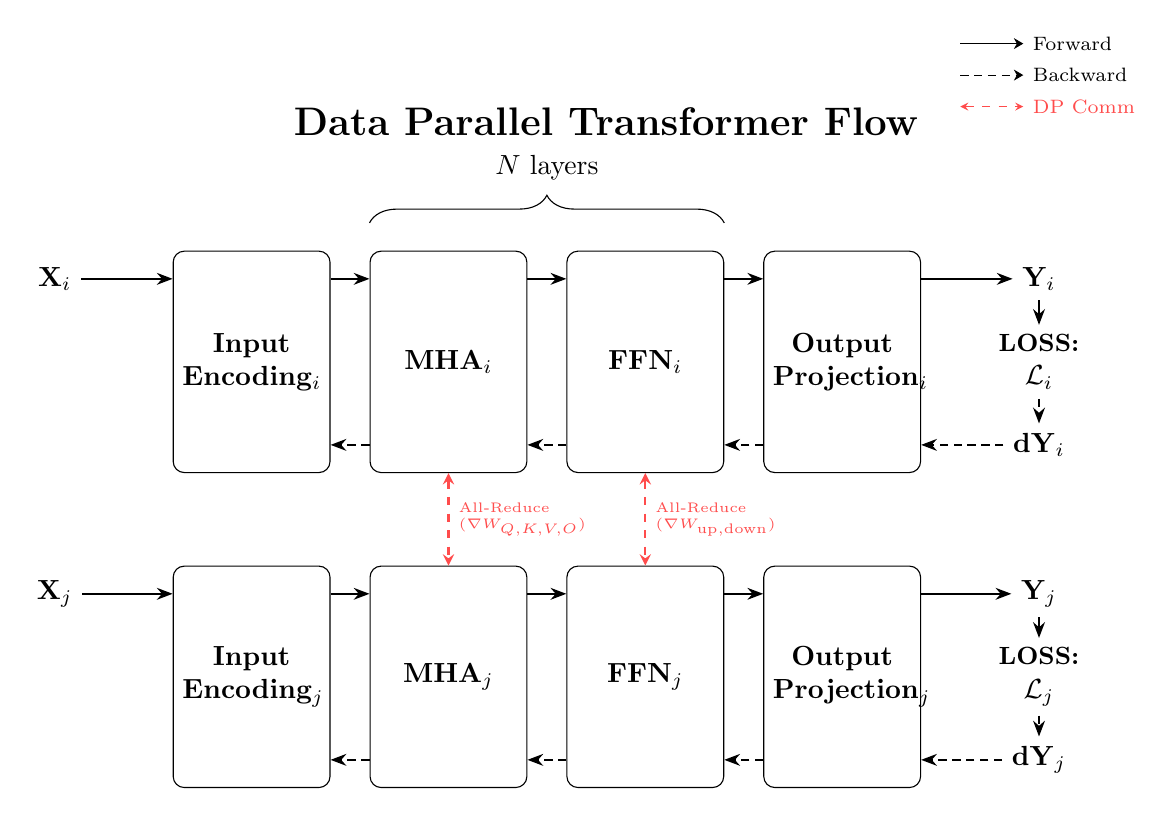
\begin{tikzpicture}[
    node distance=2.5cm,
    >=stealth,
    block/.style={rectangle, draw=black, fill=white, text width=5em, text centered, rounded corners, minimum height=8em, font=\bfseries},
    forward/.style={-{Stealth[length=2mm]}, thick, black},
    backward/.style={-{Stealth[length=2mm]}, thick, black, densely dashed},
    dpcomm/.style={<->, thick, red!70, dashed},
    io/.style={text centered, font=\bfseries}
]
    % Title
    \node[font=\Large\bfseries] at (7, 12) {Data Parallel Transformer Flow};

    % ========== Node i (Upper) ==========
    \node (input_i) [io] at (0, 10) {$\mathbf{X}_i$};
    \node (encoding_i) [block, right of=input_i, yshift=-3em] {Input\\Encoding$_i$};
    \node (mha_i) [block, right of=encoding_i] {MHA$_i$};
    \node (mlp_i) [block, right of=mha_i] {FFN$_i$};
    \node (output_i) [block, right of=mlp_i] {Output\\Projection$_i$};
    \node (pred_i) [io, right of=output_i, yshift=3em] {$\mathbf{Y}_i$};
    \node (loss_i) [align=center, io, right of=output_i] {\small LOSS:\\$\mathcal{L}_i$};
    \node (gradient_i) [io, right of=output_i, yshift=-3em] {$\mathbf{dY}_i$};

    % Forward arrows - Node i
    \draw [forward] (input_i) -- ([yshift=3em]encoding_i.west);
    \draw [forward] ([yshift=3em]encoding_i.east) -- ([yshift=3em]mha_i.west);
    \draw [forward] ([yshift=3em]mha_i.east) -- ([yshift=3em]mlp_i.west);
    \draw [forward] ([yshift=3em]mlp_i.east) -- ([yshift=3em]output_i.west);
    \draw [forward] ([yshift=3em]output_i.east) -- (pred_i);
    \draw [forward] (pred_i) -- (loss_i);
    \draw [backward] (loss_i) -- (gradient_i);

    % Backward arrows - Node i
    \draw [backward] (gradient_i) -- ([yshift=-3em]output_i.east);
    \draw [backward] ([yshift=-3em]output_i.west) -- ([yshift=-3em]mlp_i.east);
    \draw [backward] ([yshift=-3em]mlp_i.west) -- ([yshift=-3em]mha_i.east);
    \draw [backward] ([yshift=-3em]mha_i.west) -- ([yshift=-3em]encoding_i.east);

    % Brace for layer repetition - Node i
    \draw[decorate, decoration={brace, amplitude=10pt}]
        ([yshift=1.0em]mha_i.north west) -- ([yshift=1.0em]mlp_i.north east)
        node[midway, above=12pt, font=\normalsize] {$N$ layers};

    % ========== Node j (Lower) ==========
    \node (input_j) [io] at (0, 6) {$\mathbf{X}_j$};
    \node (encoding_j) [block, right of=input_j, yshift=-3em] {Input\\Encoding$_j$};
    \node (mha_j) [block, right of=encoding_j] {MHA$_j$};
    \node (mlp_j) [block, right of=mha_j] {FFN$_j$};
    \node (output_j) [block, right of=mlp_j] {Output\\Projection$_j$};
    \node (pred_j) [io, right of=output_j, yshift=3em] {$\mathbf{Y}_j$};
    \node (loss_j) [align=center, io, right of=output_j] {\small LOSS:\\$\mathcal{L}_j$};
    \node (gradient_j) [io, right of=output_j, yshift=-3em] {$\mathbf{dY}_j$};

    % Forward arrows - Node j
    \draw [forward] (input_j) -- ([yshift=3em]encoding_j.west);
    \draw [forward] ([yshift=3em]encoding_j.east) -- ([yshift=3em]mha_j.west);
    \draw [forward] ([yshift=3em]mha_j.east) -- ([yshift=3em]mlp_j.west);
    \draw [forward] ([yshift=3em]mlp_j.east) -- ([yshift=3em]output_j.west);
    \draw [forward] ([yshift=3em]output_j.east) -- (pred_j);
    \draw [forward] (pred_j) -- (loss_j);
    \draw [backward] (loss_j) -- (gradient_j);

    % Backward arrows - Node j
    \draw [backward] (gradient_j) -- ([yshift=-3em]output_j.east);
    \draw [backward] ([yshift=-3em]output_j.west) -- ([yshift=-3em]mlp_j.east);
    \draw [backward] ([yshift=-3em]mlp_j.west) -- ([yshift=-3em]mha_j.east);
    \draw [backward] ([yshift=-3em]mha_j.west) -- ([yshift=-3em]encoding_j.east);

    % ========== DP Communications ==========
    \draw [dpcomm] (mha_i.south) -- (mha_j.north) node[midway, right, font=\tiny, align=left] {All-Reduce\\$(\nabla W_{Q,K,V,O})$};
    \draw [dpcomm] (mlp_i.south) -- (mlp_j.north) node[midway, right, font=\tiny, align=left] {All-Reduce\\$(\nabla W_{\text{up},\text{down}})$};

    % Labels (Legend)
    \coordinate (legend) at ([xshift=11.5cm, yshift=8.5em]input_i);

    % Forward (작은 화살표 + 작은 글자)
    \draw[
        forward,
        -{Stealth[length=1.2mm,width=1.4mm]}, % 화살표 더 작게
        line width=0.3pt                       % 선 더 얇게
    ] (legend) -- ++(0.8,0)
      node[right, font=\scriptsize] {Forward};

    % Backward
    \draw[
        backward,
        -{Stealth[length=1.2mm,width=1.4mm]},
        line width=0.3pt
    ] ([yshift=-0.4cm]legend) -- ++(0.8,0)
      node[right, font=\scriptsize] {Backward};

    % DP Comm
    \draw[
        dpcomm,
        line width=0.3pt
    ] ([yshift=-0.8cm]legend) -- ++(0.8,0)
      node[right, font=\scriptsize] {DP Comm};
\end{tikzpicture}%
}

\clearpage

\subsection{MHA Backward under DP}
\resizebox{\linewidth}{!}{%
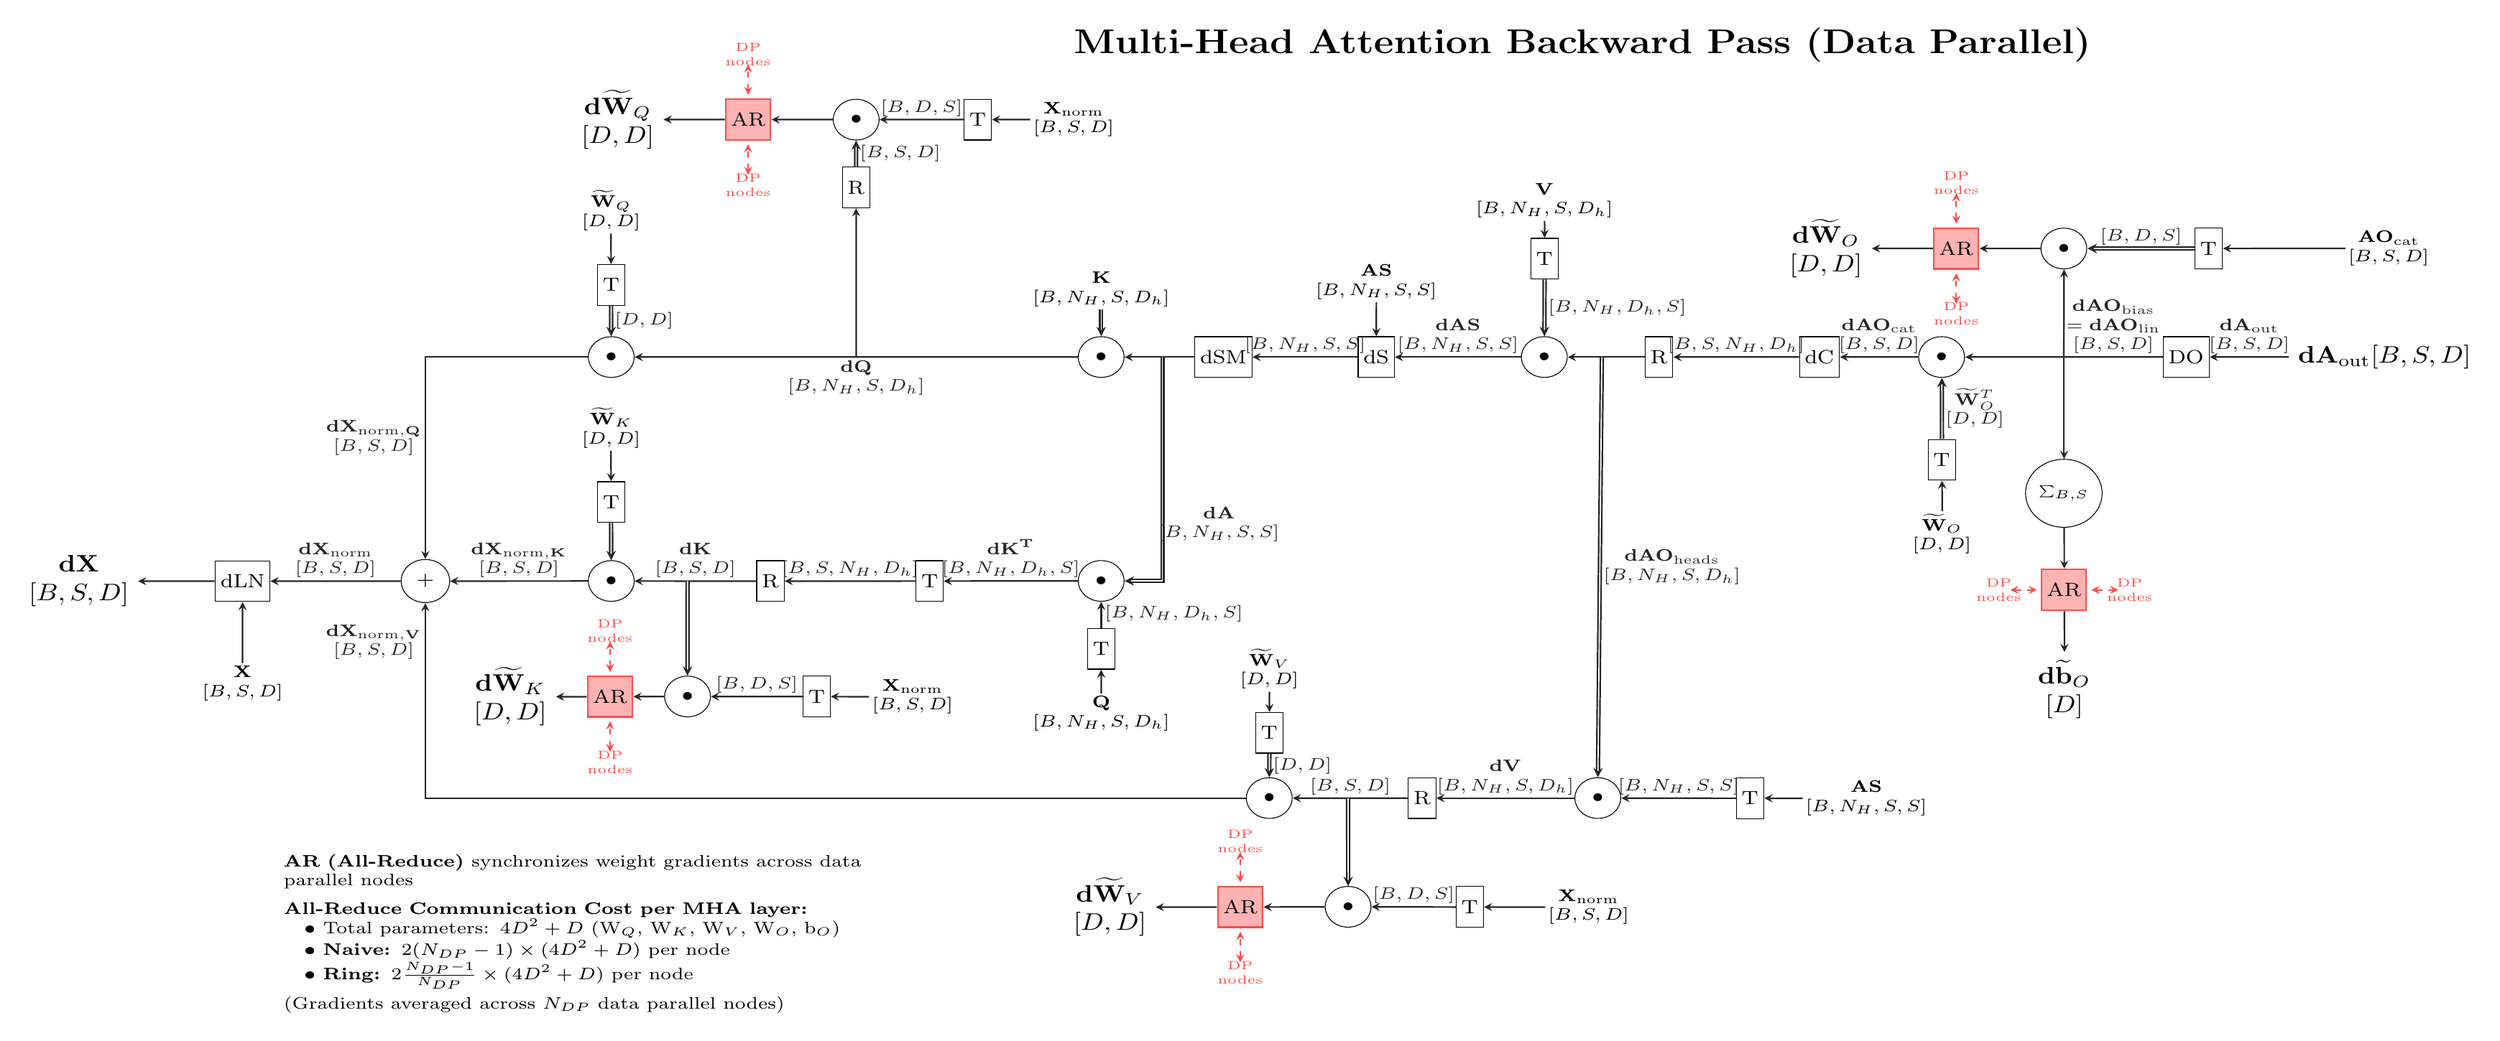
\begin{tikzpicture}[
  every node/.style={transform shape},
  >=stealth,
  auxnode/.style={draw, rectangle, fill=white, minimum height=6mm, inner sep=2pt, font=\footnotesize, align=center},
  mulnode/.style={draw, circle, fill=white, minimum size=6mm, font=\footnotesize, align=center},
  addnode/.style={draw, circle, fill=white, minimum size=6mm, font=\footnotesize, align=center},
  sumnode/.style={draw, circle, fill=white, minimum size=6mm, font=\tiny, align=center},
  arnode/.style={draw, rectangle, fill=red!30, minimum height=6mm, inner sep=2pt, font=\footnotesize, align=center, thick, draw=red!70},
  flow/.style={->, thick, black!85},
  flow2/.style={->, double, thick, black!85},
  dimlabel/.style={font=\scriptsize, inner sep=1pt, align=center},
  gradflow/.style={->, thick, black!85},
  gradweight/.style={->, thick, black!85},
  dpgradweight/.style={->, thick, black!85},
  dpcomm/.style={<->, thick, red!70, dashed}
]

\begin{scope}[xscale=1.35, yscale=1.2]

\def\yoffset{-1.0}
\def\dVXyoffset{-6.5}

\coordinate (Grad_Aout_B) at (17.5, \yoffset);
\coordinate (dDrop_center) at (15.9, \yoffset);
\coordinate (ProjGradSplit) at (14.3, \yoffset);
\coordinate (dOProj_center) at (12.7, \yoffset);
\coordinate (C_center) at (11.1, \yoffset);
\coordinate (R_center) at (9.0, \yoffset);
\coordinate (dPV_AS_calc_center) at (7.5, \yoffset);
\coordinate (dSoft_center) at (5.3, \yoffset);
\coordinate (dSM_calc_center) at (3.3, \yoffset);
\coordinate (dV_calc_center) at (8.2, \dVXyoffset+\yoffset);
\coordinate (R_V_bwd_center) at (5.9, \dVXyoffset+\yoffset);
\coordinate (dVX_calc_center) at (3.9, \dVXyoffset+\yoffset);
\coordinate (dQK_calc_Q_center) at (1.7, \yoffset);
\coordinate (dQK_calc_K_center) at (1.7, -3.3+\yoffset);
\coordinate (K_BWD_input_center) at (1.7, 1.0+\yoffset);
\coordinate (T_Q_bwd_center) at (1.7, -4.3+\yoffset);

\node[font=\Large\bfseries] at (8, 4.6+\yoffset) {Multi-Head Attention Backward Pass (Data Parallel)};

\node (Grad_Aout_B) at (18.5, \yoffset) {$\mathbf{dA}_{\text{out}}$\\$[B,S,D]$};
\node[auxnode] (DO) at (dDrop_center) {DO};
\node[mulnode] (dOProj) at (dOProj_center) {$\bullet$};

\node[auxnode] (T_WO) [below=0.9cm of dOProj] {T};
\node[dimlabel] (WO_BWD) [below=0.45cm of T_WO] {$\widetilde{\mathbf{W}}_{O}$\\$[D,D]$};

\node[mulnode] (dWO_calc) at ($(ProjGradSplit)+(0, 1.6)$) {$\bullet$};

% Add AR node before dWO
\node[arnode] (AR_WO) [left=0.8cm of dWO_calc] {AR};
\draw[dpcomm] ([yshift=-0.5cm]AR_WO.south) -- ([yshift=-0.05cm]AR_WO.south);
\draw[dpcomm] ([yshift=0.05cm]AR_WO.north) -- ([yshift=0.5cm]AR_WO.north);
\node[font=\tiny, red!70, align=center] at ([yshift=-0.65cm]AR_WO.south) {DP\\nodes};
\node[font=\tiny, red!70, align=center] at ([yshift=0.65cm]AR_WO.north) {DP\\nodes};

\node[align=center, left=0.8cm of AR_WO]
  (dWO_GRAD) {$\mathbf{d}\widetilde{\mathbf{W}}_{O}$\\$[D,D]$};
\draw[dpgradweight] (dWO_calc) -- (AR_WO);
\draw[gradflow] (AR_WO) -- (dWO_GRAD);

\node[auxnode] (T_AO_in) [right=1.4cm of dWO_calc] {T};
\node[dimlabel] (AO_in_local_label) [right=1.6cm of T_AO_in] {$\mathbf{AO}_{\text{cat}}$\\$[B,S,D]$};

\node[auxnode] (C) at (C_center) {dC};
\node[auxnode] (R) at (R_center) {R};

\node[mulnode] (dPV_AS_calc) at (dPV_AS_calc_center) {$\bullet$};
\node[auxnode] (dSoft) at (dSoft_center) {dS};
\node[auxnode] (dSM_calc) at (dSM_calc_center) {dSM};

\node[mulnode] (dQK_calc_Q) at (dQK_calc_Q_center) {$\bullet$};
\node[mulnode] (dQX_proj_calc) [left=5.8cm of dQK_calc_Q] {$\bullet$};

\node[mulnode] (dQK_calc_K) at (dQK_calc_K_center) {$\bullet$};
\node[mulnode] (dKX_proj_calc) [left=5.8cm of dQK_calc_K] {$\bullet$};

\node[dimlabel] (K_BWD_input) at (K_BWD_input_center) {$\mathbf{K}$\\$[B,N_H,S,D_h]$};
\node[auxnode] (T_Q_bwd) at (T_Q_bwd_center) {T};
\node[dimlabel] (Q_BWD_input) [below=0.35cm of T_Q_bwd] {$\mathbf{Q}$\\$[B,N_H,S,D_h]$};

\node[dimlabel] (V_FWD) [above=1.7cm of dPV_AS_calc] {$\mathbf{V}$\\$[B,N_H,S,D_h]$};
\node[auxnode] (T_V_bwd) [below=0.25cm of V_FWD] {T};

\node[mulnode] (dV_calc) at (dV_calc_center) {$\bullet$};
\node[auxnode] (T_AS_bwd) [right=1.5cm of dV_calc] {T};
\node[dimlabel] (AS_BWD_for_V) [right=0.5cm of T_AS_bwd] {$\mathbf{AS}$\\$[B,N_H,S,S]$};

\node[auxnode] (R_V_bwd) at (R_V_bwd_center) {R};
\node[mulnode] (dVX_calc) at (dVX_calc_center) {$\bullet$};

\node[auxnode] (T_WV) [above=0.35cm of dVX_calc] {T};
\node[dimlabel] (WV_BWD) [above=0.3cm of T_WV] {$\widetilde{\mathbf{W}}_{V}$\\$[D,D]$};

\node[sumnode] (Sum_dBO) [below=1.5cm of ProjGradSplit] {$\sum_{B, S}$};

% Add AR node before dBO
\node[arnode] (AR_BO) [below=0.6cm of Sum_dBO] {AR};
\draw[dpcomm] ([xshift=-0.4cm]AR_BO.west) -- ([xshift=-0.05cm]AR_BO.west);
\draw[dpcomm] ([xshift=0.05cm]AR_BO.east) -- ([xshift=0.4cm]AR_BO.east);
\node[font=\tiny, red!70, align=center] at ([xshift=-0.55cm]AR_BO.west) {DP\\nodes};
\node[font=\tiny, red!70, align=center] at ([xshift=0.55cm]AR_BO.east) {DP\\nodes};

\node[align=center] (dBO) [below=0.6cm of AR_BO] {$\mathbf{d}\widetilde{\mathbf{b}}_{O}$\\$[D]$};
\draw[dpgradweight] (Sum_dBO) -- (AR_BO);
\draw[gradflow] (AR_BO) -- (dBO);

\draw[gradflow] (Grad_Aout_B) -- (DO)
  node[dimlabel, midway, above]{$\mathbf{dA}_{\text{out}}$\\$[B,S,D]$};

\draw[gradflow] (DO) -- (dOProj)
  node[dimlabel, pos=0.25, above]{$\mathbf{dAO}_{\text{bias}}$\\$=\mathbf{dAO}_{\text{lin}}$\\$[B,S,D]$};

\draw[gradflow] (ProjGradSplit) -- (dWO_calc.south);
\draw[gradflow] (ProjGradSplit) -- ([yshift=-0.75cm]ProjGradSplit) -| (Sum_dBO.north);

\draw[gradflow] (dOProj) -- (C)
  node[dimlabel, midway, above]{$\mathbf{dAO}_{\text{cat}}$\\$[B,S,D]$};
\draw[gradflow] (C) -- (R)
  node[dimlabel, midway, above]{$[B,S,N_H,D_h]$};

\coordinate (R_split_point) at ($(dPV_AS_calc)!0.5!(R)$);
\draw[gradflow] (R.west) -- (dPV_AS_calc.east);
\draw[flow2] (R_split_point) -- (dV_calc.north)
  node[dimlabel, midway, right]{$\mathbf{dAO}_{\text{heads}}$\\$[B,N_H,S,D_h]$};

\draw[gradflow] (V_FWD.south) -- (T_V_bwd.north);
\draw[flow2] (T_V_bwd.south) -- (dPV_AS_calc.north)
  node[dimlabel, midway, right]{$[B,N_H,D_h,S]$};
\draw[gradflow] (dPV_AS_calc.west) -- (dSoft.east)
  node[dimlabel, midway, above]{$\mathbf{dAS}$\\$[B,N_H,S,S]$};

\node (AS_BWD_dS) [dimlabel, above=0.5cm of dSoft] {$\mathbf{AS}$\\$[B,N_H,S,S]$};
\draw[gradflow] (AS_BWD_dS.south) -- (dSoft.north);
\draw[gradflow] (dSoft.west) -- (dSM_calc.east)
  node[dimlabel, midway, above]{$[B,N_H,S,S]$};

\coordinate (dA_Split_X) at ($(dSM_calc_center)!0.5!(dQK_calc_Q_center)$);
\coordinate (dA_Split) at (dA_Split_X |- dQK_calc_Q.east);
\draw[gradflow] (dSM_calc.west) -- (dQK_calc_Q.east);
\draw[flow2] (dA_Split) -- (dA_Split |- dQK_calc_K.east) -- (dQK_calc_K.east)
  node[dimlabel, pos=-1.5, above, yshift=15]{$\mathbf{dA}$\\$[B,N_H,S,S]$};

\draw[flow2] (K_BWD_input.south) -- (dQK_calc_Q.north);
\draw[gradweight] (dQK_calc_Q) -- (dQX_proj_calc)
  node[dimlabel, midway, below]{$\mathbf{dQ}$\\$[B,N_H,S,D_h]$};

\node[auxnode] (T_WQ_bwd) [above=0.45cm of dQX_proj_calc] {T};
\node[dimlabel] (WQ_bwd) [above=0.45cm of T_WQ_bwd] {$\widetilde{\mathbf{W}}_{Q}$\\$[D,D]$};
\draw[flow] (WQ_bwd) -- (T_WQ_bwd);
\draw[flow2] (T_WQ_bwd.south) -- (dQX_proj_calc.north)
  node[dimlabel, midway, right]{$[D,D]$};

\draw[flow] (Q_BWD_input.north) -- (T_Q_bwd.south);
\draw[flow] (T_Q_bwd.north) -- (dQK_calc_K.south)
  node[dimlabel, pos=0.55, right]{$[B,N_H,D_h,S]$};

\node[auxnode] (T_dK) at ($(dQK_calc_K)!0.35!(dKX_proj_calc)$) {T};
\node[auxnode] (R_dK_mid) at ($(T_dK)!0.5!(dKX_proj_calc)$) {R};

\draw[gradweight] (dQK_calc_K) -- (T_dK)
  node[dimlabel, midway, above]{$\mathbf{dK^T}$\\$[B,N_H,D_h,S]$};
\draw[gradweight] (T_dK) -- (R_dK_mid)
  node[dimlabel, midway, above]{$[B,S,N_H,D_h]$};
\draw[gradweight] (R_dK_mid) -- (dKX_proj_calc)
  node[dimlabel, midway, above]{$\mathbf{dK}$\\$[B,S,D]$};

\node[auxnode] (T_WK_bwd) [above=0.55cm of dKX_proj_calc] {T};
\node[dimlabel] (WK_bwd) [above=0.45cm of T_WK_bwd] {$\widetilde{\mathbf{W}}_{K}$\\$[D,D]$};
\draw[gradflow] (WK_bwd) -- (T_WK_bwd);
\draw[flow2] (T_WK_bwd.south) -- (dKX_proj_calc.north);
\draw[gradflow] (AS_BWD_for_V.west) -- (T_AS_bwd.east);
\draw[gradflow] (T_AS_bwd.west) -- (dV_calc.east)
  node[dimlabel, midway, above]{$[B,N_H,S,S]$};
\draw[gradflow] (dV_calc.west) -- (R_V_bwd.east)
  node[dimlabel, midway, above]{$\mathbf{dV}$\\$[B,N_H,S,D_h]$};
\draw[gradflow] (R_V_bwd) -- (dVX_calc.east)
  node[dimlabel, midway, above]{$[B,S,D]$};

\draw[gradflow] (WV_BWD) -- (T_WV);
\draw[flow2] (T_WV) -- (dVX_calc.north)
  node[dimlabel, midway, right]{$[D,D]$};

\node[addnode] (Sum_dXnorm) [left=1.8cm of dKX_proj_calc] {$+$};

\draw[gradweight] (dQX_proj_calc.west) -| node[dimlabel, pos=0.7, left]{$\mathbf{dX}_{\text{norm},\mathbf{Q}}$\\$[B,S,D]$} (Sum_dXnorm.north);
\draw[gradweight] (dKX_proj_calc.west) -- node[dimlabel, midway, above]{$\mathbf{dX}_{\text{norm},\mathbf{K}}$\\$[B,S,D]$} (Sum_dXnorm.east);
\draw[gradweight] (dVX_calc.west) -| node[dimlabel, pos=0.9, left]{$\mathbf{dX}_{\text{norm},\mathbf{V}}$\\$[B,S,D]$} (Sum_dXnorm.south);

\coordinate (dV_branch) at ($(R_V_bwd.west)!0.52!(dVX_calc.east)$);
\node[mulnode] (dWV_mul) at ($(dV_branch)+(0,-1.6cm)$) {$\bullet$};
\draw[flow2] (dV_branch) -- (dWV_mul.north);

\node[auxnode] (T_Xnorm) [right=1.1cm of dWV_mul] {T};
\node[dimlabel] (Xnorm_local) [right=0.8cm of T_Xnorm] {$\mathbf{X}_{\text{norm}}$\\$[B,S,D]$};
\draw[gradflow] (Xnorm_local) -- (T_Xnorm);
\draw[gradflow] (T_Xnorm.west) -- (dWV_mul.east)
  node[dimlabel, midway, above]{$[B,D,S]$};

% Add AR node before dWV
\node[arnode] (AR_WV) [left=0.8cm of dWV_mul] {AR};
\draw[dpcomm] ([yshift=-0.5cm]AR_WV.south) -- ([yshift=-0.05cm]AR_WV.south);
\draw[dpcomm] ([yshift=0.05cm]AR_WV.north) -- ([yshift=0.5cm]AR_WV.north);
\node[font=\tiny, red!70, align=center] at ([yshift=-0.65cm]AR_WV.south) {DP\\nodes};
\node[font=\tiny, red!70, align=center] at ([yshift=0.65cm]AR_WV.north) {DP\\nodes};

\node[align=center] (dWV_out) [left=0.8cm of AR_WV] {$\mathbf{d}\widetilde{\mathbf{W}}_{V}$\\$[D,D]$};
\draw[dpgradweight] (dWV_mul.west) -- (AR_WV);
\draw[gradflow] (AR_WV) -- (dWV_out);

\coordinate (dQ_branch) at ($(dQK_calc_Q.east)!0.50!(dQX_proj_calc.west)$);
\node[mulnode] (dWQ_mul) at ($(dQ_branch)+(0,3.5cm)$) {$\bullet$};
\node[auxnode] (R_dQ_for_WQ) at ($(dWQ_mul)+(0,-1.0cm)$) {R};
\draw[gradflow]  (dQ_branch) -- (R_dQ_for_WQ.south);
\draw[flow2] (R_dQ_for_WQ.north) -- (dWQ_mul.south)
  node[dimlabel, midway, right]{$[B,S,D]$};

\node[auxnode] (T_XnormQ) [right=1.1cm of dWQ_mul] {T};
\node[dimlabel] (Xnorm_localQ) [right=0.5cm of T_XnormQ] {$\mathbf{X}_{\text{norm}}$\\$[B,S,D]$};
\draw[gradflow] (Xnorm_localQ) -- (T_XnormQ);
\draw[gradflow] (T_XnormQ.west) -- (dWQ_mul.east)
  node[dimlabel, midway, above]{$[B,D,S]$};

% Add AR node before dWQ
\node[arnode] (AR_WQ) [left=0.8cm of dWQ_mul] {AR};
\draw[dpcomm] ([yshift=-0.5cm]AR_WQ.south) -- ([yshift=-0.05cm]AR_WQ.south);
\draw[dpcomm] ([yshift=0.05cm]AR_WQ.north) -- ([yshift=0.5cm]AR_WQ.north);
\node[font=\tiny, red!70, align=center] at ([yshift=-0.65cm]AR_WQ.south) {DP\\nodes};
\node[font=\tiny, red!70, align=center] at ([yshift=0.65cm]AR_WQ.north) {DP\\nodes};

\node[align=center] (dWQ_out) [left=0.8cm of AR_WQ] {$\mathbf{d}\widetilde{\mathbf{W}}_{Q}$\\$[D,D]$};
\draw[dpgradweight] (dWQ_mul.west) -- (AR_WQ);
\draw[gradflow] (AR_WQ) -- (dWQ_out);

\coordinate (dK_branch) at ($(R_dK_mid)!0.52!(dKX_proj_calc)$);
\node[mulnode] (dWK_mul) at ($(dK_branch)+(0,-1.7cm)$) {$\bullet$};
\draw[flow2]  (dK_branch) -- (dWK_mul.north);

\node[auxnode] (T_XnormK) [right=1.2cm of dWK_mul] {T};
\node[dimlabel, right=0.5cm of T_XnormK] (Xnorm_localK) {$\mathbf{X}_{\text{norm}}$\\$[B,S,D]$};
\draw[gradflow] (Xnorm_localK) -- (T_XnormK);
\draw[gradflow] (T_XnormK.west) -- (dWK_mul.east)
  node[dimlabel, midway, above]{$[B,D,S]$};

% Add AR node before dWK
\node[arnode] (AR_WK) [left=0.4cm of dWK_mul] {AR};
\draw[dpcomm] ([yshift=-0.5cm]AR_WK.south) -- ([yshift=-0.05cm]AR_WK.south);
\draw[dpcomm] ([yshift=0.05cm]AR_WK.north) -- ([yshift=0.5cm]AR_WK.north);
\node[font=\tiny, red!70, align=center] at ([yshift=-0.65cm]AR_WK.south) {DP\\nodes};
\node[font=\tiny, red!70, align=center] at ([yshift=0.65cm]AR_WK.north) {DP\\nodes};

\node[align=center] (dWK_out) [left=0.4cm of AR_WK] {$\mathbf{d}\widetilde{\mathbf{W}}_{K}$\\$[D,D]$};
\draw[dpgradweight] (dWK_mul.west) -- (AR_WK);
\draw[gradflow] (AR_WK) -- (dWK_out);

\draw[gradflow] (WO_BWD) -- (T_WO);
\draw[flow2] (T_WO) -- (dOProj)
  node[dimlabel, midway, right]{$\widetilde{\mathbf{W}}_{O}^{T}$\\$[D,D]$};
\draw[gradflow] (AO_in_local_label) -- (T_AO_in);
\draw[flow2] (T_AO_in) -- (dWO_calc.east)
  node[dimlabel, midway, above]{$[B,D,S]$};

\node[auxnode] (dLN) [left=1.7cm of Sum_dXnorm] {dLN};
\draw[gradweight] (Sum_dXnorm.west) -- node[dimlabel, midway, above]
  {$\mathbf{dX}_{\text{norm}}$\\$[B,S,D]$} (dLN.east);

\node (dX_OUT) [align=center, left=1.0cm of dLN] {$\mathbf{dX}$\\$[B,S,D]$};
\draw[gradweight] (dLN.west) -- (dX_OUT);

\node[dimlabel] (LNCache) [below=0.9cm of dLN] {$\mathbf{X}$\\$[B,S,D]$};
\draw[gradflow] (LNCache.north) -- (dLN.south);

% Legend and explanation
    \node[align=left, font=\scriptsize, text width=8cm] at (-5, -9.5) {
      \textbf{AR (All-Reduce)} synchronizes weight gradients across data parallel nodes\\[4pt]
      \textbf{All-Reduce Communication Cost per MHA layer:}\\
      \quad • Total parameters: $4D^2 + D$ (W$_Q$, W$_K$, W$_V$, W$_O$, b$_O$)\\
      \quad • \textbf{Naive:} $2(N_{DP}-1) \times (4D^2 + D)$ per node\\
      \quad • \textbf{Ring:} $2\frac{N_{DP}-1}{N_{DP}} \times (4D^2 + D)$ per node\\[2pt]
      {\scriptsize (Gradients averaged across $N_{DP}$ data parallel nodes)}
    };

\end{scope}
\end{tikzpicture}
}

\clearpage

\subsection{MLP Backward under DP}
\noindent
\resizebox{\linewidth}{!}{%
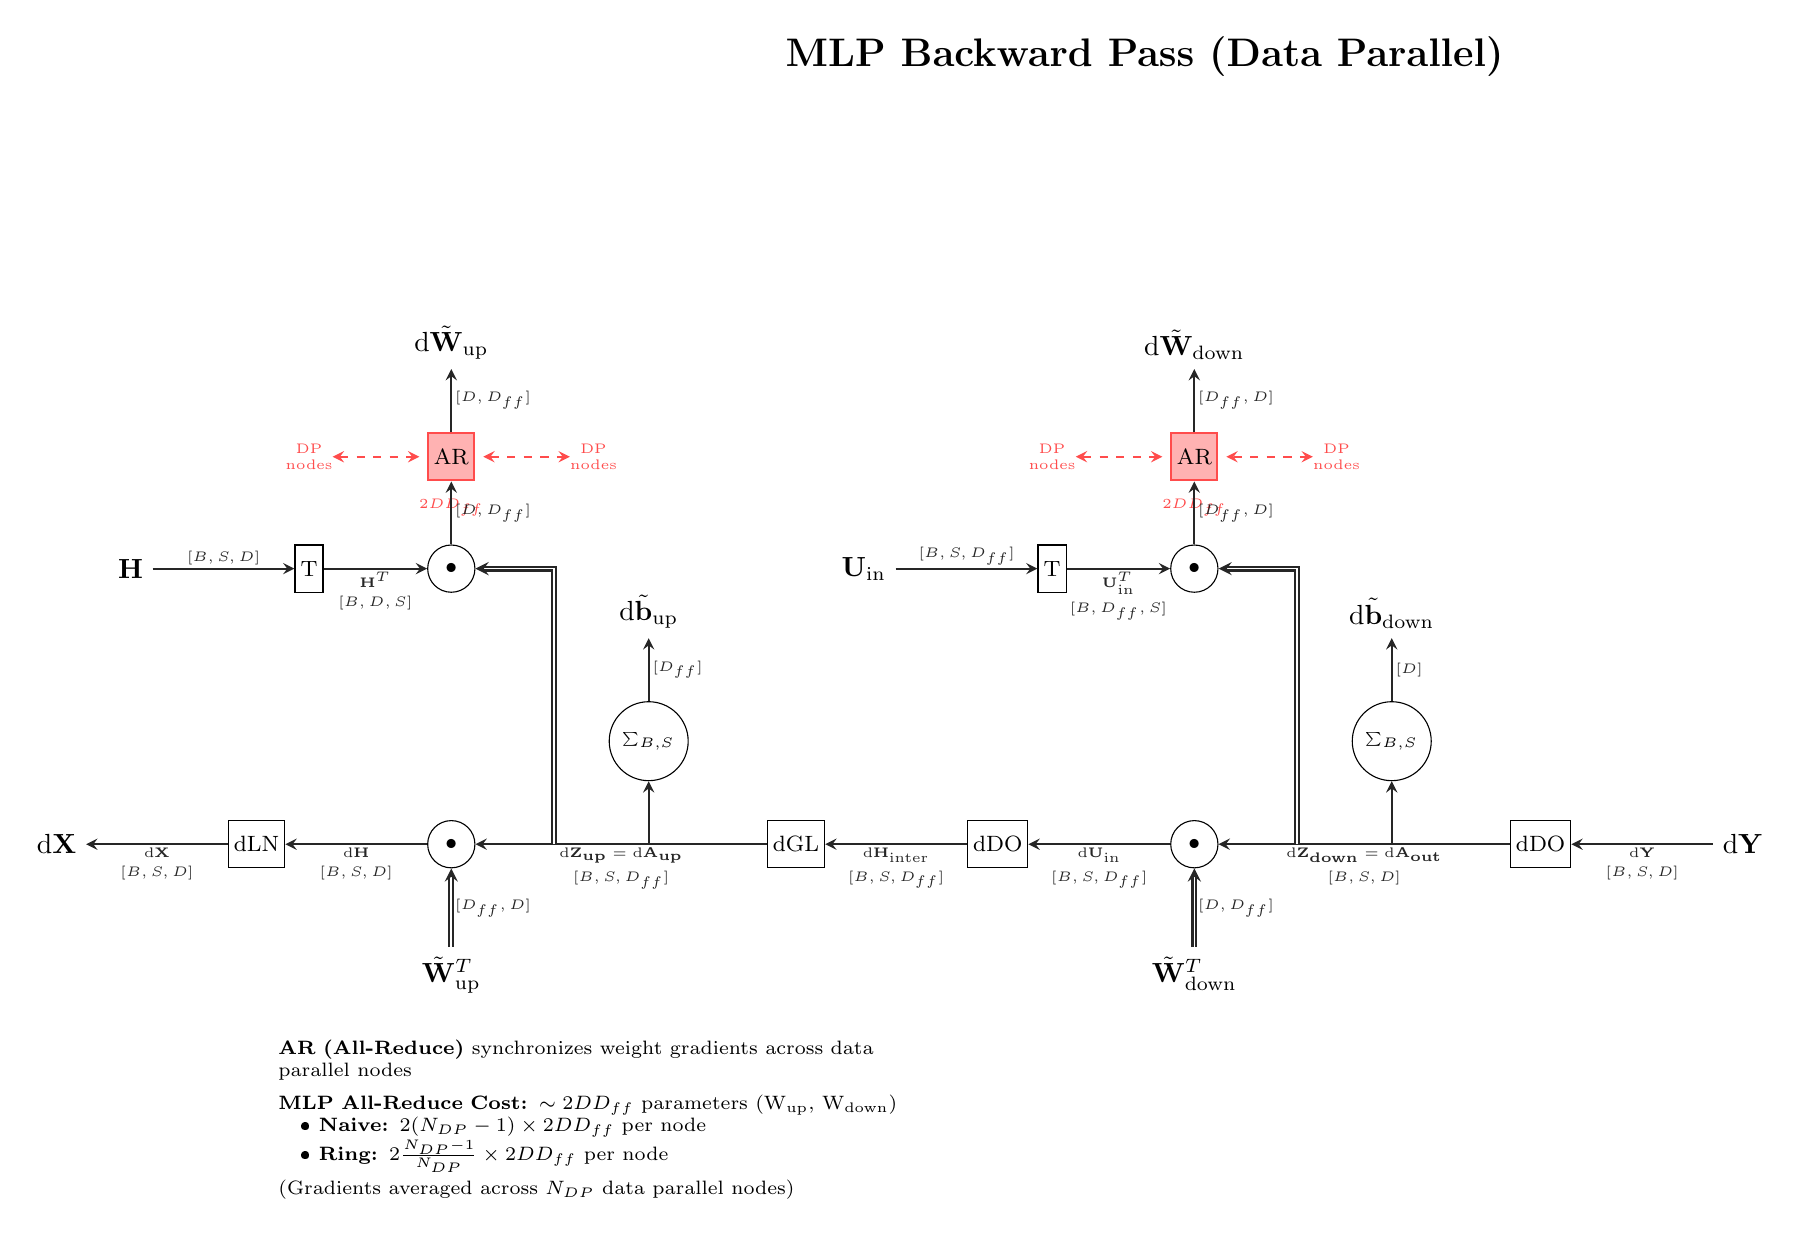
\begin{tikzpicture}[
    >=stealth,
    auxnode/.style={draw, rectangle, fill=white, minimum height=6mm, inner sep=2pt, font=\footnotesize, align=center},
    mulnode/.style={draw, circle, fill=white, minimum size=6mm, font=\footnotesize, align=center},
    addnode/.style={draw, circle, fill=white, minimum size=6mm, font=\footnotesize, align=center},
    sumnode/.style={draw, circle, fill=white, minimum size=6mm, font=\tiny, align=center},
    arnode/.style={draw, rectangle, fill=red!30, minimum height=6mm, inner sep=2pt, font=\footnotesize, align=center, thick, draw=red!70},
    flow_rev/.style={<-, thick, black!85},
    flow_dw/.style={->, thick, black!85},
    flow_act/.style={double, ->, thick, black!85},
    dimlabel/.style={font=\tiny, inner sep=1pt, align=center},
    gradlabel/.style={font=\tiny\bfseries, inner sep=1pt, align=center},
    dpgradweight/.style={->, thick, black!85},
    dpcomm/.style={<->, thick, red!70, dashed}
]
    \node[font=\Large\bfseries] at (5, 10) {MLP Backward Pass (Data Parallel)};

    \pgfmathsetmacro{\backwardoffset}{0.0}

    \node (d_MOut) at (12.6, \backwardoffset) {$\mathrm{d}\mathbf{Y}$};
    \node[auxnode] (d_Drop2) [left=1.8cm of d_MOut] {dDO};
    \draw[flow_rev] (d_Drop2) -- (d_MOut)
      node[dimlabel, midway, below]{\shortstack{$\mathrm{d}\mathbf{Y}$\\$[B,S,D]$}};

    \coordinate (split2) at ($(d_Drop2.west) + (-1.5cm, 0)$);
    \coordinate (branch_dUproj) at ($(split2) + (-1.2cm, 0)$);

    \node[sumnode] (d_SumB2) [above=0.8cm of split2] {$\sum_{B, S}$};
    \node (d_Bdown) [above=0.8cm of d_SumB2] {$\mathrm{d}\tilde{\mathbf{b}}_{\text{down}}$};
    \draw[dpgradweight] (d_SumB2) -- (d_Bdown) node[dimlabel, midway, right]{$[D]$};

    \draw[flow_rev] (d_SumB2) -- (split2);

    \node[mulnode] (d_L2Mul_in) [left=2.2cm of split2] {$\bullet$};
    \draw[flow_rev] (d_L2Mul_in) -- (d_Drop2)
      node[gradlabel, midway, below]{\shortstack{$\mathrm{d}\mathbf{Z}_{\text{down}}=\mathrm{d}\mathbf{A}_{\text{out}}$\\$[B,S,D]$}};

    \node (W_down_T) [below=1.0cm of d_L2Mul_in] {$\tilde{\mathbf{W}}_{\text{down}}^{T}$};
    \draw[flow_act] (W_down_T.north) -- (d_L2Mul_in)
      node[dimlabel, midway, right]{$[D, D_{ff}]$};

    \coordinate (L2Mul_w_y) at ($(d_L2Mul_in) + (0, 3.5cm)$);
    \node[mulnode] (d_L2Mul_w) at (L2Mul_w_y) {$\bullet$};

    % Add AR node before d_Wdown
    \node[arnode] (AR_down) [above=0.8cm of d_L2Mul_w] {AR};

    % Add communication arrows for AR_down
    \draw[dpcomm] ([xshift=-1.2cm]AR_down.west) -- ([xshift=-0.1cm]AR_down.west);
    \draw[dpcomm] ([xshift=0.1cm]AR_down.east) -- ([xshift=1.2cm]AR_down.east);
    \node[font=\tiny, red!70, align=center] at ([xshift=-1.5cm]AR_down.west) {DP\\nodes};
    \node[font=\tiny, red!70, align=center] at ([xshift=1.5cm]AR_down.east) {DP\\nodes};
    \node[font=\tiny, red!70, below=0.1cm of AR_down] {$2DD_{ff}$};

    \node (d_Wdown) [above=0.8cm of AR_down] {$\mathrm{d}\tilde{\mathbf{W}}_{\text{down}}$};
    \draw[dpgradweight] (d_L2Mul_w) -- (AR_down) node[dimlabel, midway, right]{$[D_{ff}, D]$};
    \draw[flow_dw] (AR_down) -- (d_Wdown) node[dimlabel, midway, right]{$[D_{ff}, D]$};

    \draw[flow_act] (branch_dUproj.north) |- (d_L2Mul_w.east);

    \node[auxnode] (Uin_T) at ($(d_L2Mul_w.west) + (-1.5cm, 0)$) {T};
    \draw[flow_dw] (Uin_T) -- (d_L2Mul_w)
      node[dimlabel, midway, below]{\shortstack{$\mathbf{U}_{\text{in}}^T$\\$[B, D_{ff}, S]$}};
    \node (Uin_aux) [left=1.8cm of Uin_T] {$\mathbf{U}_{\text{in}}$};
    \draw[flow_dw] (Uin_aux) -- (Uin_T) node[dimlabel, midway, above]{\shortstack{$[B,S,D_{ff}]$}};

    \node[auxnode] (d_Drop1) [left=1.8cm of d_L2Mul_in] {dDO};
    \draw[flow_rev] (d_Drop1) -- (d_L2Mul_in)
      node[dimlabel, midway, below]{\shortstack{$\mathrm{d}\mathbf{U}_{\text{in}}$\\$[B,S,D_{ff}]$}};

    \node[auxnode] (d_Act) [left=1.8cm of d_Drop1] {dGL};
    \draw[flow_rev] (d_Act) -- (d_Drop1)
      node[dimlabel, midway, below]{\shortstack{$\mathrm{d}\mathbf{H}_{\text{inter}}$\\$[B,S,D_{ff}]$}};

    \coordinate (split1) at ($(d_Act.west) + (-1.5cm, 0)$);
    \coordinate (branch_dHpre) at ($(split1) + (-1.2cm, 0)$);

    \node[sumnode] (d_SumB1) [above=0.8cm of split1] {$\sum_{B, S}$};
    \node (d_Bup) [above=0.8cm of d_SumB1] {$\mathrm{d}\tilde{\mathbf{b}}_{\text{up}}$};
    \draw[dpgradweight] (d_SumB1) -- (d_Bup) node[dimlabel, midway, right]{$[D_{ff}]$};

    \draw[flow_rev] (d_SumB1) -- (split1);

    \node[mulnode] (d_L1Mul_in) [left=2.2cm of split1] {$\bullet$};
    \draw[flow_rev] (d_L1Mul_in) -- (d_Act)
      node[gradlabel, midway, below]{\shortstack{$\mathrm{d}\mathbf{Z}_{\text{up}}=\mathrm{d}\mathbf{A}_{\text{up}}$\\$[B,S,D_{ff}]$}};

    \node (W_up_T) [below=1.0cm of d_L1Mul_in] {$\tilde{\mathbf{W}}_{\text{up}}^{T}$};
    \draw[flow_act] (W_up_T.north) -- (d_L1Mul_in)
      node[dimlabel, midway, right]{$[D_{ff}, D]$};

    \coordinate (L1Mul_w_y) at ($(d_L1Mul_in) + (0, 3.5cm)$);
    \node[mulnode] (d_L1Mul_w) at (L1Mul_w_y) {$\bullet$};

    % Add AR node before d_Wup
    \node[arnode] (AR_up) [above=0.8cm of d_L1Mul_w] {AR};

    % Add communication arrows for AR_up
    \draw[dpcomm] ([xshift=-1.2cm]AR_up.west) -- ([xshift=-0.1cm]AR_up.west);
    \draw[dpcomm] ([xshift=0.1cm]AR_up.east) -- ([xshift=1.2cm]AR_up.east);
    \node[font=\tiny, red!70, align=center] at ([xshift=-1.5cm]AR_up.west) {DP\\nodes};
    \node[font=\tiny, red!70, align=center] at ([xshift=1.5cm]AR_up.east) {DP\\nodes};
    \node[font=\tiny, red!70, below=0.1cm of AR_up] {$2DD_{ff}$};

    \node (d_Wup) [above=0.8cm of AR_up] {$\mathrm{d}\tilde{\mathbf{W}}_{\text{up}}$};
    \draw[dpgradweight] (d_L1Mul_w) -- (AR_up) node[dimlabel, midway, right]{$[D, D_{ff}]$};
    \draw[flow_dw] (AR_up) -- (d_Wup) node[dimlabel, midway, right]{$[D, D_{ff}]$};

    \draw[flow_act] (branch_dHpre.north) |- (d_L1Mul_w.east);

    \node[auxnode] (Znorm_T) at ($(d_L1Mul_w.west) + (-1.5cm, 0)$) {T};
    \draw[flow_dw] (Znorm_T) -- (d_L1Mul_w)
      node[dimlabel, midway, below]{\shortstack{$\mathbf{H}^T$\\$[B, D, S]$}};
    \node (Znorm_aux) [left=1.8cm of Znorm_T] {$\mathbf{H}$};
    \draw[flow_dw] (Znorm_aux) -- (Znorm_T) node[dimlabel, midway, above]{\shortstack{$[B,S,D]$}};

    \node[auxnode] (d_LN2) [left=1.8cm of d_L1Mul_in] {dLN};
    \draw[flow_rev] (d_LN2) -- (d_L1Mul_in)
      node[dimlabel, midway, below]{\shortstack{$\mathrm{d}\mathbf{H}$\\$[B,S,D]$}};

    \node (d_MIn) [left=1.8cm of d_LN2] {$\mathrm{d}\mathbf{X}$};
    \draw[flow_rev] (d_MIn) -- (d_LN2)
      node[dimlabel, midway, below]{\shortstack{$\mathrm{d}\mathbf{X}$\\$[B,S,D]$}};

    % Legend and explanation
    \node[align=left, font=\scriptsize, text width=8cm] at (-2, -3.5) {
      \textbf{AR (All-Reduce)} synchronizes weight gradients across data parallel nodes\\[4pt]
      \textbf{MLP All-Reduce Cost:} $\sim 2DD_{ff}$ parameters (W$_{\text{up}}$, W$_{\text{down}}$)\\
      \quad • \textbf{Naive:} $2(N_{DP}-1) \times 2DD_{ff}$ per node\\
      \quad • \textbf{Ring:} $2\frac{N_{DP}-1}{N_{DP}} \times 2DD_{ff}$ per node\\[2pt]
      {\scriptsize (Gradients averaged across $N_{DP}$ data parallel nodes)}
    };

\end{tikzpicture}%
}

\clearpage

% ==========================================================
% 7. Hybrid Data + Tensor Parallelism (DP + TP)
% ==========================================================
\section{Hybrid Data + Tensor Parallelism (DP + TP)}

We combine tensor parallelism within each node (or group of devices)
with data parallelism across groups. This section explains how the two
forms of parallelism interact in both forward and backward passes.

\subsection{DP+TP Overview and Communication Patterns}
\resizebox{\linewidth}{!}{%
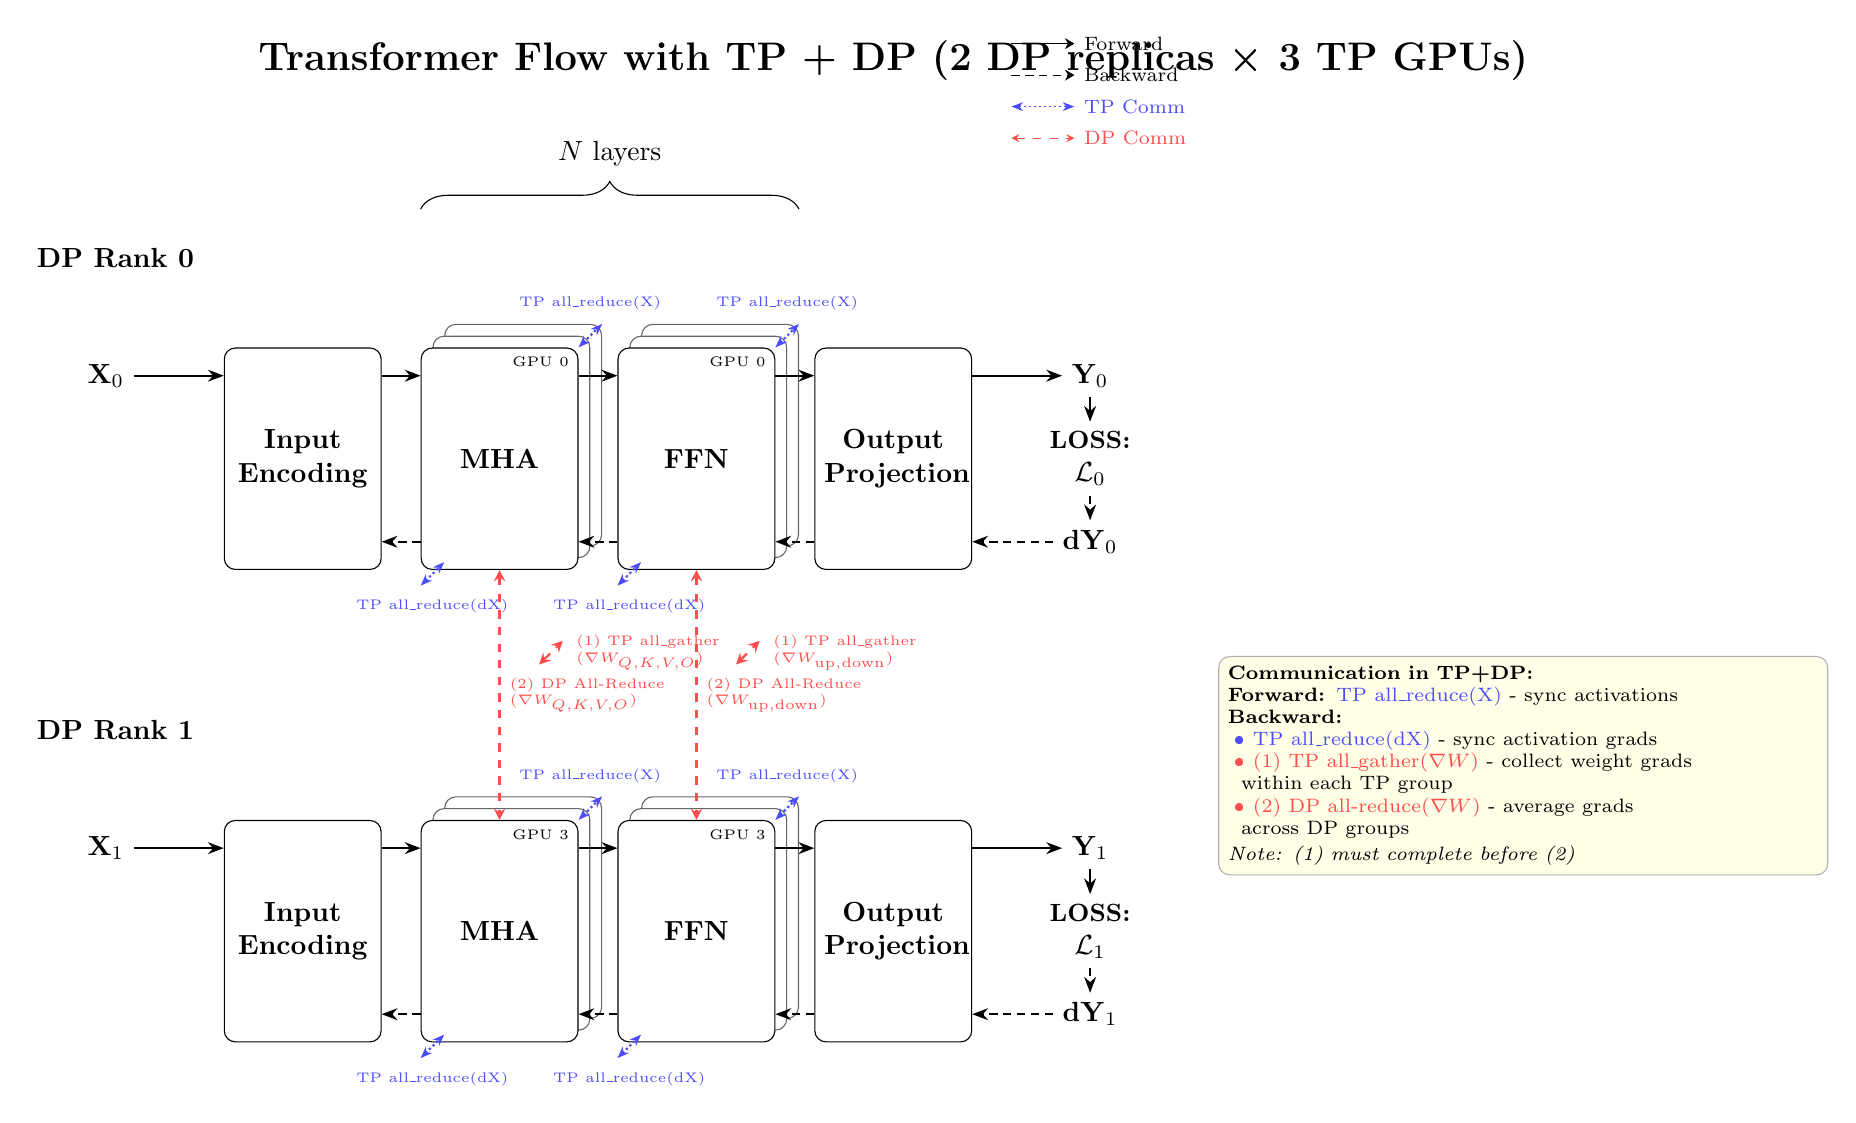
\begin{tikzpicture}[
    node distance=2.5cm,
    >=stealth,
    block/.style={rectangle, draw=black, fill=white, text width=5em, text centered, rounded corners, minimum height=8em, font=\bfseries},
    blockstack/.style={rectangle, draw=black!60, fill=white, text width=5em, text centered, rounded corners, minimum height=8em},
    forward/.style={-{Stealth[length=2mm]}, thick, black},
    backward/.style={-{Stealth[length=2mm]}, thick, black, densely dashed},
    tpcomm/.style={{Stealth[length=1.5mm]}-{Stealth[length=1.5mm]}, thick, blue!70, densely dotted},
    dpcomm/.style={<->, thick, red!70, dashed},
    io/.style={text centered, font=\bfseries}
]
    % Title
    \node[font=\Large\bfseries] at (10, 14) {Transformer Flow with TP + DP (2 DP replicas × 3 TP GPUs)};

    % ========== DP Replica 0 (Upper) ==========
    \node[font=\normalsize\bfseries, anchor=west] at (-1, 11.5) {DP Rank 0};

    \node (input_0) [io] at (0, 10) {$\mathbf{X}_0$};
    \node (encoding_0) [block, right of=input_0, yshift=-3em] {Input\\Encoding};

    % MHA blocks (3 stacked) - TP Group 0
    \node (mha3_0) [blockstack, right of=encoding_0, xshift=0.3cm, yshift=0.3cm] {};
    \node (mha2_0) [blockstack, right of=encoding_0, xshift=0.15cm, yshift=0.15cm] {};
    \node (mha_0) [block, right of=encoding_0] {MHA};
    \node[font=\tiny, anchor=north east] at (mha_0.north east) {GPU 0};

    % FFN blocks (3 stacked) - TP Group 0
    \node (mlp3_0) [blockstack, right of=mha_0, xshift=0.3cm, yshift=0.3cm] {};
    \node (mlp2_0) [blockstack, right of=mha_0, xshift=0.15cm, yshift=0.15cm] {};
    \node (mlp_0) [block, right of=mha_0] {FFN};
    \node[font=\tiny, anchor=north east] at (mlp_0.north east) {GPU 0};

    \node (output_0) [block, right of=mlp_0] {Output\\Projection};
    \node (pred_0) [io, right of=output_0, yshift=3em] {$\mathbf{Y}_0$};
    \node (loss_0) [align=center, io, right of=output_0] {\small LOSS:\\$\mathcal{L}_0$};
    \node (gradient_0) [io, right of=output_0, yshift=-3em] {$\mathbf{dY}_0$};

    % Forward arrows - DP Rank 0
    \draw [forward] (input_0) -- ([yshift=3em]encoding_0.west);
    \draw [forward] ([yshift=3em]encoding_0.east) -- ([yshift=3em]mha_0.west);
    \draw [forward] ([yshift=3em]mha_0.east) -- ([yshift=3em]mlp_0.west);
    \draw [forward] ([yshift=3em]mlp_0.east) -- ([yshift=3em]output_0.west);
    \draw [forward] ([yshift=3em]output_0.east) -- (pred_0);
    \draw [forward] (pred_0) -- (loss_0);
    \draw [backward] (loss_0) -- (gradient_0);

    % Backward arrows - DP Rank 0
    \draw [backward] (gradient_0) -- ([yshift=-3em]output_0.east);
    \draw [backward] ([yshift=-3em]output_0.west) -- ([yshift=-3em]mlp_0.east);
    \draw [backward] ([yshift=-3em]mlp_0.west) -- ([yshift=-3em]mha_0.east);
    \draw [backward] ([yshift=-3em]mha_0.west) -- ([yshift=-3em]encoding_0.east);

    % TP Communications - DP Rank 0
    % Forward All-Reduce
    \draw [tpcomm] (mha_0.north east) -- ([xshift=0.3cm, yshift=0.3cm]mha_0.north east);
    \node[font=\tiny, blue!70, anchor=south] at ([xshift=0.15cm, yshift=0.35cm]mha_0.north east) {TP all\_reduce(X)};

    \draw [tpcomm] (mlp_0.north east) -- ([xshift=0.3cm, yshift=0.3cm]mlp_0.north east);
    \node[font=\tiny, blue!70, anchor=south] at ([xshift=0.15cm, yshift=0.35cm]mlp_0.north east) {TP all\_reduce(X)};

    % Backward All-Reduce - dX
    \draw [tpcomm] ([yshift=-0.2cm]mlp_0.south west) -- ([xshift=0.3cm, yshift=0.1cm]mlp_0.south west);
    \node[font=\tiny, blue!70, anchor=north] at ([xshift=0.15cm, yshift=-0.25cm]mlp_0.south west) {TP all\_reduce(dX)};

    \draw [tpcomm] ([yshift=-0.2cm]mha_0.south west) -- ([xshift=0.3cm, yshift=0.1cm]mha_0.south west);
    \node[font=\tiny, blue!70, anchor=north] at ([xshift=0.15cm, yshift=-0.25cm]mha_0.south west) {TP all\_reduce(dX)};

    % Backward All-Gather for gradients - positioned on right side, before DP all-reduce
    \draw [dpcomm] ([xshift=-0.5cm, yshift=-1.2cm]mlp_0.south east) -- ([xshift=-0.2cm, yshift=-0.9cm]mlp_0.south east);
    \node[font=\tiny, red!70, anchor=west, align=left] at ([xshift=-0.15cm, yshift=-1.05cm]mlp_0.south east) {(1) TP all\_gather\\$(\nabla W_{\text{up},\text{down}})$};

    \draw [dpcomm] ([xshift=-0.5cm, yshift=-1.2cm]mha_0.south east) -- ([xshift=-0.2cm, yshift=-0.9cm]mha_0.south east);
    \node[font=\tiny, red!70, anchor=west, align=left] at ([xshift=-0.15cm, yshift=-1.05cm]mha_0.south east) {(1) TP all\_gather\\$(\nabla W_{Q,K,V,O})$};

    % Brace for layer repetition - DP Rank 0
    \draw[decorate, decoration={brace, amplitude=10pt}]
        ([yshift=5.0em]mha_0.north west) -- ([xshift=0.3cm, yshift=5.0em]mlp_0.north east)
        node[midway, above=12pt, font=\normalsize] {$N$ layers};

    % ========== DP Replica 1 (Lower) ==========
    \node[font=\normalsize\bfseries, anchor=west] at (-1, 5.5) {DP Rank 1};

    \node (input_1) [io] at (0, 4) {$\mathbf{X}_1$};
    \node (encoding_1) [block, right of=input_1, yshift=-3em] {Input\\Encoding};

    % MHA blocks (3 stacked) - TP Group 1
    \node (mha3_1) [blockstack, right of=encoding_1, xshift=0.3cm, yshift=0.3cm] {};
    \node (mha2_1) [blockstack, right of=encoding_1, xshift=0.15cm, yshift=0.15cm] {};
    \node (mha_1) [block, right of=encoding_1] {MHA};
    \node[font=\tiny, anchor=north east] at (mha_1.north east) {GPU 3};

    % FFN blocks (3 stacked) - TP Group 1
    \node (mlp3_1) [blockstack, right of=mha_1, xshift=0.3cm, yshift=0.3cm] {};
    \node (mlp2_1) [blockstack, right of=mha_1, xshift=0.15cm, yshift=0.15cm] {};
    \node (mlp_1) [block, right of=mha_1] {FFN};
    \node[font=\tiny, anchor=north east] at (mlp_1.north east) {GPU 3};

    \node (output_1) [block, right of=mlp_1] {Output\\Projection};
    \node (pred_1) [io, right of=output_1, yshift=3em] {$\mathbf{Y}_1$};
    \node (loss_1) [align=center, io, right of=output_1] {\small LOSS:\\$\mathcal{L}_1$};
    \node (gradient_1) [io, right of=output_1, yshift=-3em] {$\mathbf{dY}_1$};

    % Forward arrows - DP Rank 1
    \draw [forward] (input_1) -- ([yshift=3em]encoding_1.west);
    \draw [forward] ([yshift=3em]encoding_1.east) -- ([yshift=3em]mha_1.west);
    \draw [forward] ([yshift=3em]mha_1.east) -- ([yshift=3em]mlp_1.west);
    \draw [forward] ([yshift=3em]mlp_1.east) -- ([yshift=3em]output_1.west);
    \draw [forward] ([yshift=3em]output_1.east) -- (pred_1);
    \draw [forward] (pred_1) -- (loss_1);
    \draw [backward] (loss_1) -- (gradient_1);

    % Backward arrows - DP Rank 1
    \draw [backward] (gradient_1) -- ([yshift=-3em]output_1.east);
    \draw [backward] ([yshift=-3em]output_1.west) -- ([yshift=-3em]mlp_1.east);
    \draw [backward] ([yshift=-3em]mlp_1.west) -- ([yshift=-3em]mha_1.east);
    \draw [backward] ([yshift=-3em]mha_1.west) -- ([yshift=-3em]encoding_1.east);

    % TP Communications - DP Rank 1
    % Forward All-Reduce
    \draw [tpcomm] (mha_1.north east) -- ([xshift=0.3cm, yshift=0.3cm]mha_1.north east);
    \node[font=\tiny, blue!70, anchor=south] at ([xshift=0.15cm, yshift=0.35cm]mha_1.north east) {TP all\_reduce(X)};

    \draw [tpcomm] (mlp_1.north east) -- ([xshift=0.3cm, yshift=0.3cm]mlp_1.north east);
    \node[font=\tiny, blue!70, anchor=south] at ([xshift=0.15cm, yshift=0.35cm]mlp_1.north east) {TP all\_reduce(X)};

    % Backward All-Reduce - dX
    \draw [tpcomm] ([yshift=-0.2cm]mlp_1.south west) -- ([xshift=0.3cm, yshift=0.1cm]mlp_1.south west);
    \node[font=\tiny, blue!70, anchor=north] at ([xshift=0.15cm, yshift=-0.25cm]mlp_1.south west) {TP all\_reduce(dX)};

    \draw [tpcomm] ([yshift=-0.2cm]mha_1.south west) -- ([xshift=0.3cm, yshift=0.1cm]mha_1.south west);
    \node[font=\tiny, blue!70, anchor=north] at ([xshift=0.15cm, yshift=-0.25cm]mha_1.south west) {TP all\_reduce(dX)};

    % Backward All-Gather for gradients - positioned on right side, before DP all-reduce
    % \draw [dpcomm] ([xshift=0.5cm, yshift=-1.2cm]mlp_1.south east) -- ([xshift=0.8cm, yshift=-0.9cm]mlp_1.south east);
    % \node[font=\tiny, red!70, anchor=west, align=left] at ([xshift=0.85cm, yshift=-1.05cm]mlp_1.south east) {(1) TP all\_gather\\$(\nabla W_{\text{up},\text{down}})$};

    % \draw [dpcomm] ([xshift=0.5cm, yshift=-1.2cm]mha_1.south east) -- ([xshift=0.8cm, yshift=-0.9cm]mha_1.south east);
    % \node[font=\tiny, red!70, anchor=west, align=left] at ([xshift=0.85cm, yshift=-1.05cm]mha_1.south east) {(1) TP all\_gather\\$(\nabla W_{Q,K,V,O})$};

    % ========== DP Communications (Between TP Groups) ==========
    \draw [dpcomm] (mha_0.south) -- (mha_1.north) node[midway, right, font=\tiny, align=left, red!70] {(2) DP All-Reduce\\$(\nabla W_{Q,K,V,O})$};
    \draw [dpcomm] (mlp_0.south) -- (mlp_1.north) node[midway, right, font=\tiny, align=left, red!70] {(2) DP All-Reduce\\$(\nabla W_{\text{up},\text{down}})$};

    % Communication Order Annotation
    \node[font=\scriptsize, align=left, text width=7.5cm, draw=black!30, fill=yellow!10, rounded corners] at ([xshift=15.5cm, yshift=10em]encoding_1.south) {
        \textbf{Communication in TP+DP:}\\
        \textbf{Forward:} \textcolor{blue!70}{TP all\_reduce(X)} - sync activations\\
        \textbf{Backward:}\\
        \hspace{0.3em}\textcolor{blue!70}{• TP all\_reduce(dX)} - sync activation grads\\
        \hspace{0.3em}\textcolor{red!70}{• (1) TP all\_gather($\nabla W$)} - collect weight grads\\
        \hspace{0.6em}within each TP group\\
        \hspace{0.3em}\textcolor{red!70}{• (2) DP all-reduce($\nabla W$)} - average grads\\
        \hspace{0.6em}across DP groups\\[0.2em]
        \textit{Note: (1) must complete before (2)}
    };

    % Labels (Legend)
    \coordinate (legend) at ([xshift=11.5cm, yshift=12em]input_0);

    % Forward
    \draw[forward, -{Stealth[length=1.2mm,width=1.4mm]}, line width=0.3pt] (legend) -- ++(0.8,0)
      node[right, font=\scriptsize] {Forward};

    % Backward
    \draw[backward, -{Stealth[length=1.2mm,width=1.4mm]}, line width=0.3pt] ([yshift=-0.4cm]legend) -- ++(0.8,0)
      node[right, font=\scriptsize] {Backward};

    % TP Comm
    \draw[tpcomm, line width=0.3pt] ([yshift=-0.8cm]legend) -- ++(0.8,0)
      node[right, font=\scriptsize] {TP Comm};

    % DP Comm
    \draw[dpcomm, line width=0.3pt] ([yshift=-1.2cm]legend) -- ++(0.8,0)
      node[right, font=\scriptsize] {DP Comm};

\end{tikzpicture}%
}

\clearpage

% ==========================================================
% 8. Summary and Practical Takeaways
% ==========================================================
\section{Summary and Practical Takeaways}

We summarize the main ideas:
\begin{itemize}
  \item How a Transformer layer operates as a composition of
        embedding, MHA, MLP, and output projection blocks.
  \item How tensor shapes evolve through forward and backward passes.
  \item How single-node execution extends to tensor parallelism, data
        parallelism, and their combination.
\end{itemize}

We also highlight how these diagrams can be used as a reference when
designing or debugging large-scale Transformer training and inference
systems.

\end{document}
